%%% Reset counters for the footnotes and compound numbering
%\setcounter{compound}{0}
\stepcounter{cmpreset}
\captionsetup[figure]{list=no} % hide figures from list in experimental section

 \chapter{Extension of Catalytic Single Carbon Ring Expansion to Complex
 Molecule Synthesis}
 \label{chp:singlecarbon}
 %\thispagestyle{empty}
 \pagebreak
 
\section{Introduction} 
\doublespacing 
Natural product total synthesis
often provides the impetus for developing new organic methodologies and can
function as a proving ground for evaluating the utility of existing synthetic
tools.\footnote{For a review on the impact of total synthesis on the
field of organic chemistry see: \frenchspacing{Nicolaou, K. C.; Vourloumis, D.;
Winssinger, N.; Baran, P. S. The Art and Science of Total Synthesis at the Dawn
of the Twenty-First Century. \textit{Angew. Chem. Int. Ed.} \textbf{2000},
\textit{39}, 44-122.}} Our group recently disclosed methodology for catalytic
and regioselective single carbon ring expansion of $\alpha$,$\alpha$-substituted
cyclobutanones with
trimethylsilyldiazomethane.\footnote{\frenchspacing{Dabrowski, J. A.; Moebius,
D. C.; Wommack, A. J.; Kornahrens, A. F.; Kingsbury, J. S. Catalytic and
Regioselective Ring Expansion of Arylcyclobutanones with
Trimethylsilyldiazomethane. Ligand-Dependent Entry to $\beta$-Ketosilane or
Enolsilane Adducts. \textit{Org. Lett.} \textbf{2010}, \textit{12}, 3598-3601.}
\label{ref:cdabrowski}} To prove the generality of our new mild and catalytic approach, we aimed to
apply this strategic ring expansion reaction in the context of natural product synthesis. Several biologically active sesquiterpenoid quinone natural products
bearing a \textit{cis}-fused decalin core were selected, and we set out with the
intent of developing a general strategy to access the \textit{cis}-decalin
carbon framework common to the avarane\footnote{(a) \frenchspacing{Marcos, I.
S.; Conde, A.; Moro, R. F.; Basabe, P.; Diez, D.; Urones, J. G.
Quinone/Hydroquinone Sesquiterpenes. \textit{Mini-Rev. Org. Chem.}
\textbf{2010}, \textit{7}, 230-254}. (b) \frenchspacing{Thomson, R. H.
\textit{Naturally Occuring Quinones IV: Recent Advances}, 4th ed.; Chapman \&
Hall: New York, 1997}.} family of natural products (\refscheme{strategydecalin}). By designing a
route in which the pendant aryl group could be tuned, a number of different natural products and
their analogs could be accessed through single carbon homologation of a cyclopentanone intermediate
(\ref{cmp:baa}\ce{->}\ref{cmp:bab}). 

\begin{Scheme}[H]
  \centering
  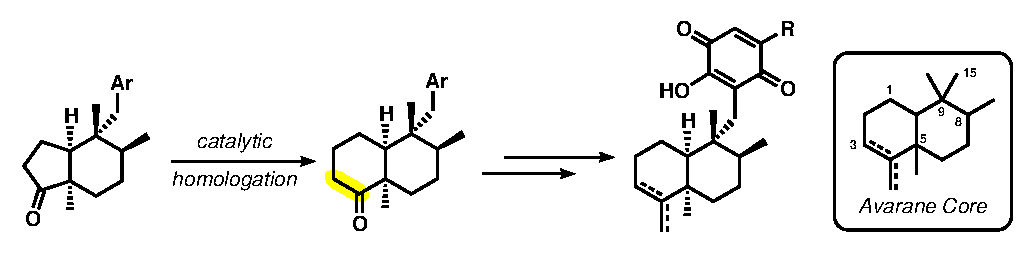
\includegraphics[scale=0.8]{chp_singlecarbon/images/strategydecalin}
\begin{textblock}{1}(1.7,-0.25) \cmp{baa} \end{textblock}
\begin{textblock}{1}(7.6,-0.25) \cmp{bab} \end{textblock}
  \caption{Access to \textit{cis}-decalin natural products by single-carbon ring
  expansion.}
  \label{sch:strategydecalin}
\end{Scheme}
 This chapter will discuss progress made towards sesquiterpene
 quinone natural products with an emphasis on ring expansion methodology development.
 Improvements have been
made to our original reaction conditions for cyclobutanones, such that the
arguably more challenging cyclopentanone\footnote{The order of reactivity for
the ring expansion of cycloalkanones with diazomethane based on literature
precedents and qualitative observations is: cyclobutanone $\approx$
cyclohexanone $>$ cycloheptanone $>$ cyclopentanone. \frenchspacing{Gutsche, C.
D. The Reaction of Diazomethane and Its Derivatives with Aldehydes and Ketones.
\textit{Org. React.} \textbf{1954}, \textit{8}, 364-403}. \label{ref:cgutsche}}
substrates are now readily homologated to the corresponding cyclohexanones with high yields and
regioselectivities. Methods developed in our group showcase the first examples
of catalytic ring expansions with trimethylsilyldiazomethane and
represent a significant improvement over existing protocols. A history of previous
single carbon homologation methods with diazoalkanes was presented in chapter \ref{chp:diazobkg}.
Examples of diazoalkane-based single carbon homologation in complex molecule synthesis are presented
in the section that follows.

\pagebreak

 \section{Diazoalkane Single Carbon Homologation in Complex
Molecules}
Single-carbon ring expansion is a powerful synthetic disconnection and has been
successfully implemented in a number of complex molecule syntheses. As discussed in Chapter
\ref{chp:diazobkg}, diazoalkane based ring expansions have made significant advances over the years.
More recent methodologies, based on the findings of Shioiri\footnote{{\frenchspacing Hashimoto, N.;
Aoyama, T.; Shioiri, T. New Methods and Reagents in Organic Synthesis. 10.
Trimethylsilyldiazomethane (TMSCHN$_2$). A New, Stable, and Safe Reagent for the Homologation of
Ketones. \textit{Tetrahedron Lett.} \textbf{1980}, \textit{21}, 4619-4622.} \label{ref:cshioiri}}
and Yamamoto,\footnote{(a)
\frenchspacing{Maruoka, K.; Concepcion, A. B.; Yamamoto, H. Selective Homologation of Ketones and Aldehydes with Diazoalkanes Promoted by Organoaluminum Reagents. \textit{Synthesis}. \textbf{1994}, 1283-1290}. (b) \frenchspacing{Maruoka, K.; Concepcion, A. B.; Yamamoto, H. Organoaluminum-Promoted Homologation of Ketones with Diazoalkanes. \textit{J.
Org. Chem.} \textbf{1994}, \textit{59}, 4725-4726.} \label{ref:cyamamoto}} have made their way into
the total syntheses of several natural and synthetic biologically active complex molecules. Chemists will often construct or purchase
the lower homologue of a ring system, utilize known methods to build up
complexity, and then implement a key ring expansion event to access the target ring size. In the
section that follows, several examples of sucessful single-carbon homologation
in the context of complex substrates will be presented. 

Polycyclic ether marine natural products, especially those belonging to
the brevotoxin family, have been linked to
cases of neurotoxic shellfish poising.\footnote{\frenchspacing{Watkins, S. M.;
Reich, A.; Fleming, L. E.; Hammond, R. Neurotoxic Shellfish Poisoning. \textit{Mar. Drugs.} \textbf{2008},
\textit{6}, 431-55.}} The discovery of these molecules and their
corresponding biological effects lead to the development of new synthetic
strategies to access the \textit{trans}-fused 6-- to 9-membered polycyclic ether
framework common to these natural products.\footnote{\frenchspacing{Nicolaou, K. C.; Yang, Z.; Shi, G.;
Gunzner, J. L.; Agrios, K. A.; G\"artner, P. Total Synthesis of Brevetoxin A.
\textit{Nature.} \textbf{1998}, \textit{392}, 264-269.}} In 1997, Mori and
coworkers published a strategy based on iterative ring expansion of the corresponding 6-membered lower homologue to access 7-membered oxepane rings.\footnote{(a) \frenchspacing{Mori, Y.; Yaegashi, K.; Furukawa, H. Stereoselective Synthesis of the 6,7,6- and 6,7,7-Ring Systems of Polycyclic Ethers by 6-endo Cyclization and Ring Expansion. \textit{Tetrahedron.} \textbf{1997}, \textit{53}, 12917-12932}. (b) \frenchspacing{Mori, Y. Yaegashi, K.; Furukawa, H. Oxiranyl Anions in
Organic Synthesis: Application to the Synthesis of Hemibrevetoxin B. \textit{J.
Am. Chem. Soc.} \textbf{1997}, \textit{119}, 4557-4558}. (c)
\frenchspacing{Mori, Y.; Nogami, K.; Hayashi, H.; Noyori, R.
Sulfonyl-Stabilized Oxiranyllithium-Based Approach to Polycyclic Ethers.
Convergent Synthesis of the ABCDEF-Ring System of Yessotoxin and Adriatoxin.
\textit{J. Org. Chem.} \textbf{2003}, \textit{68}, 9050-9060}.} Table
\ref{tbl:mori} shows the results of a Lewis acid screen on model substrate
\ref{cmp:baq}. The highest yields and regioselectivites were observed with the
Shioiri\crossref{ref:cshioiri} conditions at $-$78~\degc~(entry 4). Preferential
migration of the anticipated less substituted bond, followed by 1,3-Brook
rearrangement\footnote{{\frenchspacing Brook, A. G. Some Molecular Rearrangements of Organosilicon
Compounds. \textit{Acc. Chem. Res.} \textbf{1974}, \textit{7}, 77-84.} \label{ref:cbrook}} yielded
\ref{cmp:bar}, which was deprotected with PPTS to afford the target oxepane \ref{cmp:bas} in 76\%
yield over two steps.\footnote{For a more complete discussion of regioselectivity preferences see Chapter \ref{chp:diazobkg}.} \begin{table}[t] \centering
\vspace{10pt}
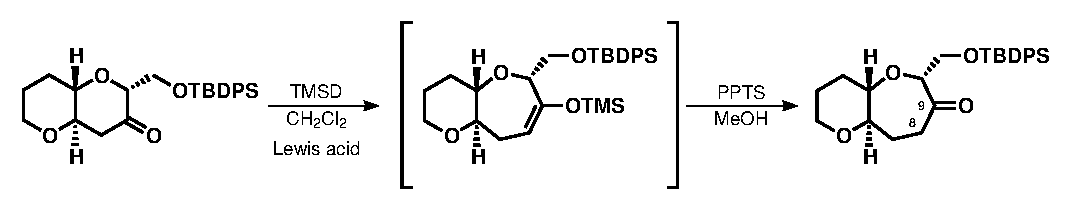
\includegraphics[scale=0.8]{chp_singlecarbon/images/morione} \\
\begin{textblock}{1}(2.2,-0.7) \cmp{baq} \end{textblock}
\begin{textblock}{1}(9.4,-0.7) \cmp{bar} \end{textblock}
\begin{textblock}{1}(16.5,-0.7) \cmp{bas} \end{textblock}
\vspace{10pt}
{\small
\begin{tabular}{cccccc}
\toprule
entry & Lewis acid & conditions & \ref{cmp:bas} (\%) & 8-keto isomer (\%) & rr 
\\
\midrule
1&\ce{Et2AlCl}&$-$78~\degc, 2h & 40 & 7 & 5.7:1\\
2&\ce{Me3Al}&$-$78~\degc, 1.5h & 48 & 32 & 1.5:1 \\
3&\ce{BF3.Et2O}&$-$20~\degc, 1h & 56 & 11 & 5.1:1 \\
\rowcolor{gray!15}4&\ce{BF3.Et2O}&$-$78~\degc, 1h & 76 & 5 & 15:1\\
\bottomrule
\end{tabular}
}
\caption{Lewis acid and condition screen for polyether model substrate.}
\label{tbl:mori}
\end{table}

Satisfied with these model
studies, Mori utilized this ring expansion strategy in a formal synthesis of
hemibrevetoxin B (\refscheme{mori}). Lewis acid mediated ring
closure of \ref{cmp:bat} and deoxygenation afforded cyclohexanone homologation
substrate \ref{cmp:bau}. Single carbon ring expansion under highly optimized
conditions yielded the first 7-membered ether \ref{cmp:bav} in a 67\% yield.
After a series of manipulations, \ref{cmp:baw} was obtained and subsequently
homologated to introduce the second 7-membered ring. Mori was able to
sucessfully implement two regioselective single-carbon ring expansion events and
secure intermediate \ref{cmp:bax}, which could then be elaborated to the target
product (\ce{->}\ref{cmp:bay}). 

\begin{Scheme}[t]
  \centering 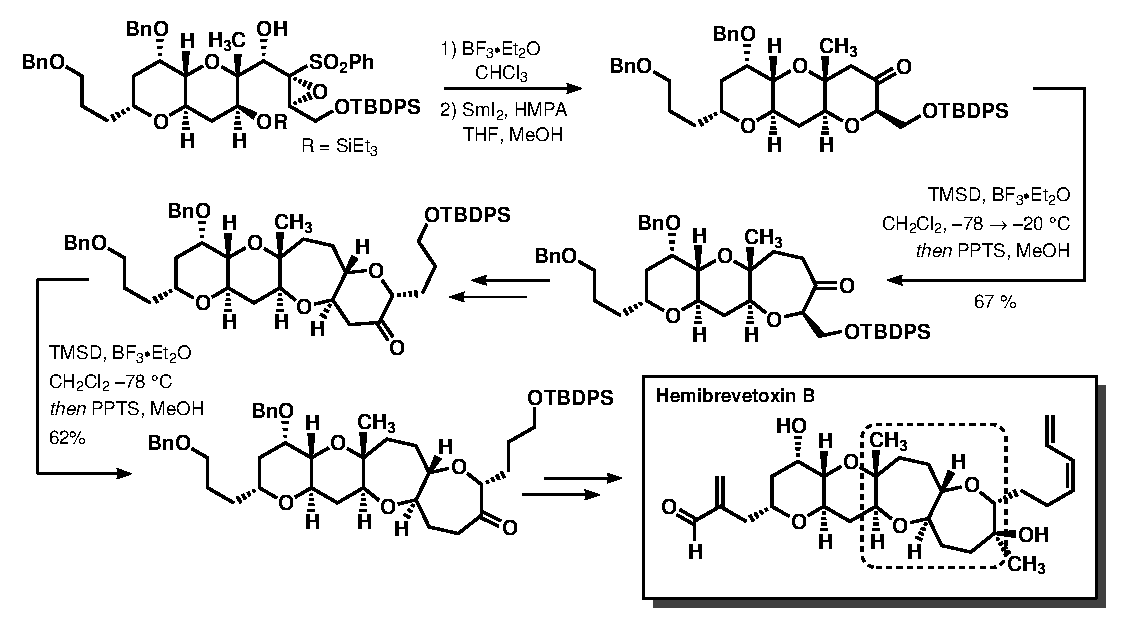
\includegraphics[scale=0.8]{chp_singlecarbon/images/moritwo}
  \caption{Mori's formal synthesis of hemibrevetoxin B featuring iterative
  ring expansions.}
  \begin{textblock}{1}(3.3,-8) \cmp{bat} \end{textblock}
  \begin{textblock}{1}(13.7,-8) \cmp{bau} \end{textblock}
  \begin{textblock}{1}(12.3,-4.7) \cmp{bav} \end{textblock}
  \begin{textblock}{1}(4,-4.8) \cmp{baw} \end{textblock}
  \begin{textblock}{1}(5.5,-1.2) \cmp{bax} \end{textblock}
  \begin{textblock}{1}(13,-1) \cmp{bay} \end{textblock}
  \label{sch:mori}
\end{Scheme}

In Pazos' 2009 synthesis of isolaurepan, a similar homologation strategy was
employed to produce the oxepane ring system found in the desired target
(\refscheme{pazos}).\footnote{\frenchspacing{Pazos, G.; P\'erez, M.
G\'andara, Z.; G\'omez, G.; Fall, Y. A New, Enantioselective Synthesis of (+)-Isolaurepan.
\textit{Tetrahedron Lett.} \textbf{2009}, \textit{50}, 5285-5287.}} Treatment of
$\alpha$-tertiary substituted cyclohexanone \ref{cmp:bbk} with \ce{BF3.Et2O} and
TMSD afforded cycloheptanone \ref{cmp:bbl} in a respectable 60\% isolated yield.
Again, preferential migration of the less substituted carbon atom was observed
to deliver a 7.5:1 mixture of regioisomers. The late stage homologation product
\ref{cmp:bbl} was then advanced to the target isolaurepan (\ref{cmp:bbm}) with
four additional steps.
\begin{Scheme}[h]
  \centering \includegraphics[scale=0.8]{chp_singlecarbon/images/pazos}
  \caption{Pazos' total synthesis of isolaurepan.}
\begin{textblock}{1}(2,-0.6) \cmp{bbk} \end{textblock}
\begin{textblock}{1}(9,-0.4) \cmp{bbl} \end{textblock}
\begin{textblock}{1}(16,-0.7) \cmp{bbm} \end{textblock}	
  \label{sch:pazos}
\end{Scheme}

% The migratory apptitudes observed in the aforementioned syntheses follow
% a pattern that is distinct from those observed in the classic Baeyer-Villager
% reaction. In the Baeyer-Villager reaction, migration of the more substituted carbon
% substitutent is typically observed.\footnote{(a) \frenchspacing{Doering, W.
% E.; Speers, L. The Peracetic Acid Cleavage of Unsymmetrical Ketones. \textit{J.
% Am. Chem. Soc.} \textbf{1950}, \textit{72}, 5515-5518}. (b)
% \frenchspacing{Crudden, C. M.; Chen, A. C.; Calhoun, L. A. A Demonstration of the Primary Stereoelectronic Effect in the Baeyer-Villiger Oxidation of $\alpha$-Fluorocyclohexanones. \textit{Angew. Chem. Int. Ed.} \textbf{2000},
% \textit{39}, 2851-2855.}} This observation is rationalized by
% disposing the substrate such that the peracid bond is oriented antiperiplanar to
% the larger substituent. This effect has also been attributed to the ability of
% the migrating group to stabilize a buildup of partial positive charge in the
% transition state. The regiochemical outcome in these
% two syntheses was however, not unprecedented. Both
% Gutsche\crossref{ref:gutschetwo} and Shioiri\crossref{ref:shioiri} demonstrated
% that the less substituted bond migrates preferentially with diazomethane and
% TMSD. Greene\crossref{ref:greene} had previously demonstrated that
% $\alpha$,$\alpha$-dichlorocyclobutanones show a preference for migration of the
% more electron rich bond, however, the stereoelectronic disposition of the
% diazoalkane appears to a more important determining factor in less
% electronically biased situations.
\begin{Scheme}[t] \centering 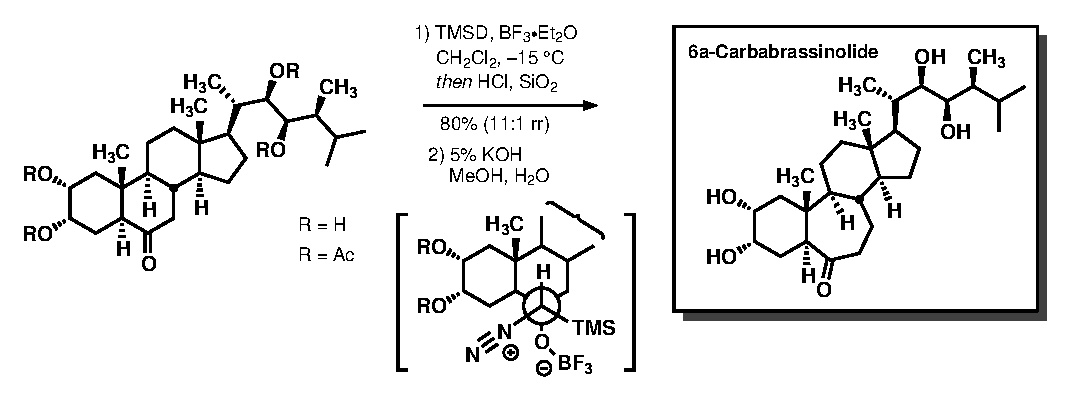
\includegraphics[scale=0.8]{chp_singlecarbon/images/seto}
  \caption{Seto's synthesis of 6a-Carbabrassinolide.}
  \begin{textblock}{1}(4.5,-2.95) \cmp{baz} \end{textblock}
  \begin{textblock}{1}(4.5,-2.4) \cmp{bba} \end{textblock}
  \begin{textblock}{1}(7.7,-0.8) \cmp{bbb} \end{textblock}
  \begin{textblock}{1}(16.5,-2.5) \cmp{bbc} \end{textblock}
  \label{sch:seto}
\end{Scheme}
In Seto's synthesis of 6a-carbabrassinolide, a regioselective ring expansion
facilitated concise access to the target steroid derivative
(\refscheme{seto}).\footnote{\frenchspacing{Seto, H.; Fujioka, S.;
Koshino, H.; Hayasaka, H.; Shimizu, T.; Yoshida, S.; Watanabe, T. Synthesis and
Biological Activity of 6a-Carbabrassinolide: B-Ring Homologation of
6-Oxo-Steroid to 6-Oxo-7a-Homosteroid with Trimethylsilyldiazomethane-Boron
Trifluoride Etherate. \textit{Tetrahedron Lett.} \textbf{1999}, \textit{40},
2359-2362.}} Global acetate protection (\ref{cmp:baz} \ce{->} \ref{cmp:bba})
prevents formation of methyl ethers by O-H insertion. Seto proposes that the
diazoalkane adds to place the bulky TMS group away from the ring fusion and with
the proton oriented inside of the ring system (\ref{cmp:bbb}). This simple
model, based on minimization of steric interactions, correctly predicts the
regiochemical outcome in the previous two examples as well. Seto obtains the desired
heptanone in 11:1 regioselectivity and an excellent 80\% yield. Base-mediated
global acetate deprotection delivered 6a-carbabrassinolide (\ref{cmp:bbc}). 


In Smalley's approach to the novel antiviral compound TAK-779 (\refscheme{smalley}), a decagram
scale highly regioselective single carbon ring expansion was employed to form the crucial benzofused
7-membered carbocycle.\footnote{\frenchspacing{Smalley, T. L. A Ring Expansion Strategy in Antiviral
Synthesis: A Novel Approach to TAK-779. \textit{Synthetic Commun.} \textbf{2004}, \textit{34},
1973-1980.}} Starting from inexpensive and commercially available 7-methoxy-1-tetralone
(\ref{cmp:bbd}), biaryl tetralone \ref{cmp:bbe} was quickly accessed through a three step sequence. 
Ring expansion with \ce{BF3.Et2O} and TMSD afforded the desired suberone \ref{cmp:bbf} in multi-gram
quantities as a single regioisomer by $^1$H NMR spectroscopy. The high preference for migration of the aryl bond can be rationalized by an electronic orbital overlap
argument. Diazoalkane insertion reactions with aldehydes typically afford ketone products, formed by
preferential migration of the carbonyl C-H bond.\footnote{For a lead reference on
aldehyde homologations with diazoalkanes see: {\frenchspacing Wommack, A. J.; Moebius, D. C.;
Travis, A. L.; Kingsbury, J. S. Diverse Alkanones by Catalytic Carbon Insertion into the Formyl C-H
Bond. Concise Access to the Natural Precursor of Achyrofuran. \textit{Org. Lett.} \textbf{2009},
\textit{11}, 3202-3205.}} The spherical, non-directional nature of the hydrogen \textit{s} orbital
allows for facile migration. In Smalley's example, the migrating carbon center is sp$^2$ hybridized,
resulting in a less directional orbital that can overlap more readily with the \ce{C-N} $\sigma^*$
orbital. This migration preference was also consistent with a previous report by House that showed a
strong preference for phenyl versus alkyl migration with diazomethane and
\ce{BF3.Et2O}.\footnote{See Table \ref{tbl:housereg} on page \pageref{tbl:housereg} and:
{\frenchspacing House, H. O.; Grubbs, E. J.; Gannon, W. F. The Reaction of Ketones with
Diazomethane. \textit{J. Am. Chem. Soc.} \textbf{1960}, \textit{82}, 4099-4106.}} The synthesis was
completed in 5 additional steps, providing scalable access to TAK-779 (\ref{cmp:bbg}).
\begin{Scheme}[t]
  \centering 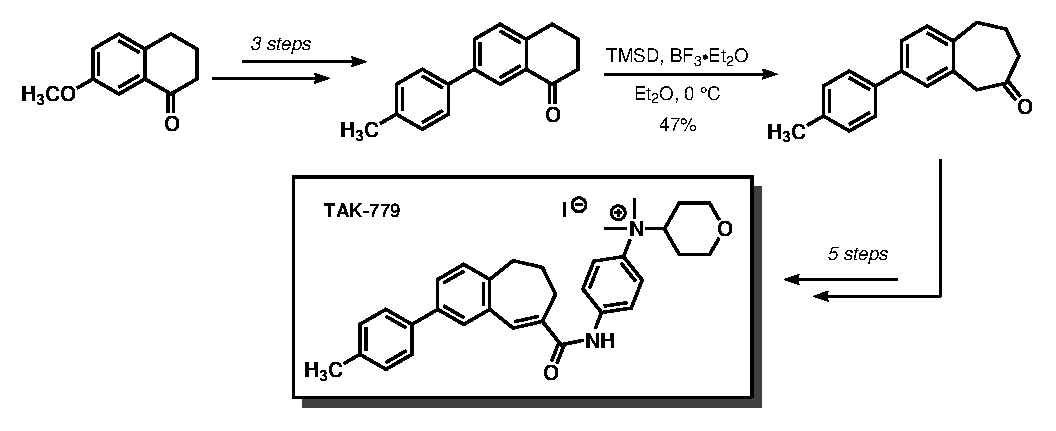
\includegraphics[scale=0.8]{chp_singlecarbon/images/smalley}
  \caption{Smalley's approach to TAK-779 with highly regioselective ring
  expansion.}
  \begin{textblock}{1}(2,-5.2) \cmp{bbd} \end{textblock}
  \begin{textblock}{1}(9,-5.2) \cmp{bbe} \end{textblock}
  \begin{textblock}{1}(16.8,-5.2) \cmp{bbf} \end{textblock}
  \begin{textblock}{1}(8.4,-1) \cmp{bbg} \end{textblock}
  \label{sch:smalley}
\end{Scheme}

The reaction of diazomethane with $\alpha$,$\beta$-unsaturated carbonyl compounds under classical
protic conditions has been shown to produce pyrazoline products arising from 1,3-dipolar
cycloaddtions.\footnote{See reference \ref{ref:cgutsche} for further details.\\
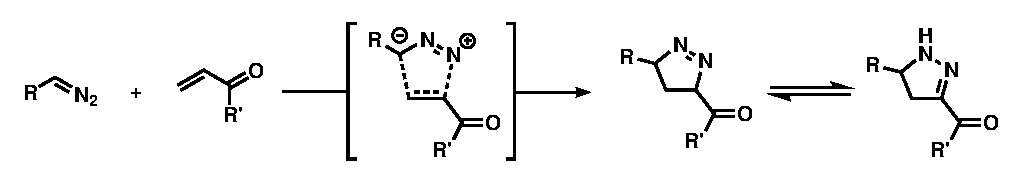
\includegraphics[scale=0.7]{chp_singlecarbon/images/alphabetaunsat}} Limited examples of
$\alpha$,$\beta$-unsaturated carbonyl substrates undergoing ring expansion in the presence of Lewis
acid catalysts have been reported. It was not until the introduction of
Lewis acids for diazoalkane ring expansion that these types of substrates
were accessible.\footnote{{\frenchspacing Johnson, W.
S.; Neeman, M.; Birkeland, S. P.; Fedoruk, N. A. The Acid-catalyzed Reaction of Diazomethane with Some
$\alpha$,$\beta$-Unsaturated Ketones. \textit{J. Am. Chem. Soc.} \textbf{1962}, \textit{84},
989-992.}} In Dr\`ege's synthesis of the cyathin terpenoid framework, an intramolecular Heck
reaction (\ref{cmp:bbh} \ce{->} \ref{cmp:bbi}, Scheme \ref{sch:drege}) set the stage for a rare
$\alpha$,$\beta$-unsaturated cyclohexenone ring expansion.\footnote{\frenchspacing{(a) Dr\`ege, E.; Morgant, G.; Desma\"ele, D.
Asymmetric Synthesis of the Tricyclic Core of Cyathin Diterpenoids via Intramolecular Heck Reaction.
\textit{Tetrahedron Lett.} \textbf{2005}, \textit{46}, 7263-7266}. (b) \frenchspacing{Dr\`ege, E.;
Tominiaux, C.; Morgant, G.; Desma\"ele, D. Synthetic Studies on Cyathin Terpenoids: Enantioselective
Synthesis of the Tricyclic Core of Cyathin through Intramolecular Heck Cyclisation. \textit{Eur. J.
Org. Chem.} \textbf{2006}, 4825-4840.}}  Under the Yamamoto\crossref{ref:cyamamoto} conditions,
cyclohexenone \ref{cmp:bbi} was smoothly converted to the desired cycloheptanone \ref{cmp:bbj} in a
60\% isolated yield with 6:1 regioselectivity.

\begin{Scheme}[t]
  \centering 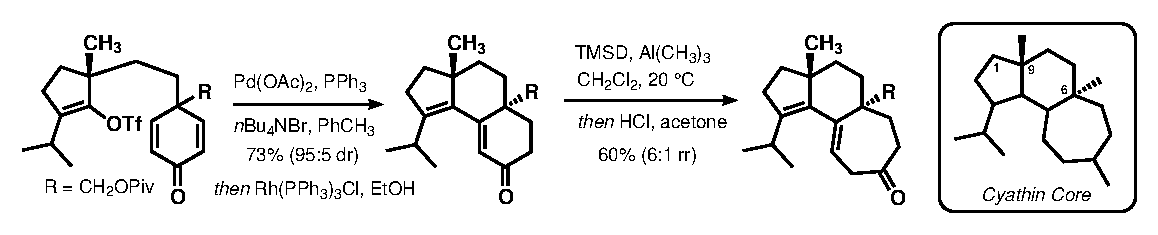
\includegraphics[scale=0.8]{chp_singlecarbon/images/drege}
  \caption{Dr\`ege's approach to the cyathin terpenoid carbon framework.}
\begin{textblock}{1}(1.2,-0.2) \cmp{bbh} \end{textblock}
\begin{textblock}{1}(9,-0.6) \cmp{bbi} \end{textblock}
\begin{textblock}{1}(13.5,-0.6) \cmp{bbj} \end{textblock}
  \label{sch:drege}
\end{Scheme}

In arguably one of the most challenging single
carbon homologations to date, the Snyder group attempted to
homologate an exceptionally crowded $\alpha$,$\alpha'$-disubstituted
cyclohexanone during their synthesis of
Rippertenol (\refscheme{snyder}).\footnote{\frenchspacing{Snyder,
S. A.; Wespe, D. A.; von Hof, J. M. A Concise, Stereocontrolled Total Synthesis
of Rippertenol. \textit{J. Am. Chem. Soc.} \textbf{2011}, \textit{133},
8850-8853.}} A Lewis acid mediated inverse demand Diels-Alder reaction between
electron deficient diene \ref{cmp:bbn} and ketene acetal \ref{cmp:bbo} afforded
the carbon framework of the six membered ring (\ce{->}\ref{cmp:bbp}) that would later
be subjected to single carbon homologation. Two further steps, Lombardo-Takai
olefination with an acidic workup and hydrogenation, unmasked the ketone for ring
expansion (\ref{cmp:bbp} \ce{->} \ref{cmp:bbq}). Extensive screening lead to modified
Shioiri\crossref{ref:cshioiri} conditions as the optimium means to obtain
cycloheptanone \ref{cmp:bbr}, although it was only recovered in 21\% yield under
highly optimized conditions. The regiochemical outcome was not anticipated,
however, it was of little consequence as the ketone was removed in subsequent
steps. To avoid epimerization of the adjacent methyl stereocenter, a two-step
reduction radical deoxgenation strategy followed by silyl deprotection delivered
the target natural product \ref{cmp:bbs}. 

The Synder synthesis of rippertenol and other examples that have been presented
illustrate a need for more mild and catalytic methods to accomplish single
carbon ring expansions. Although a number of the syntheses showcase successful
and high yielding ring expansions, none of the examples are catalytic. The
sections that follow will detail our work to develop and successfully implement
the first mild and catalytic ring expansion methodology in the context of
complex molecule synthesis.

\begin{Scheme}[t]
  \centering 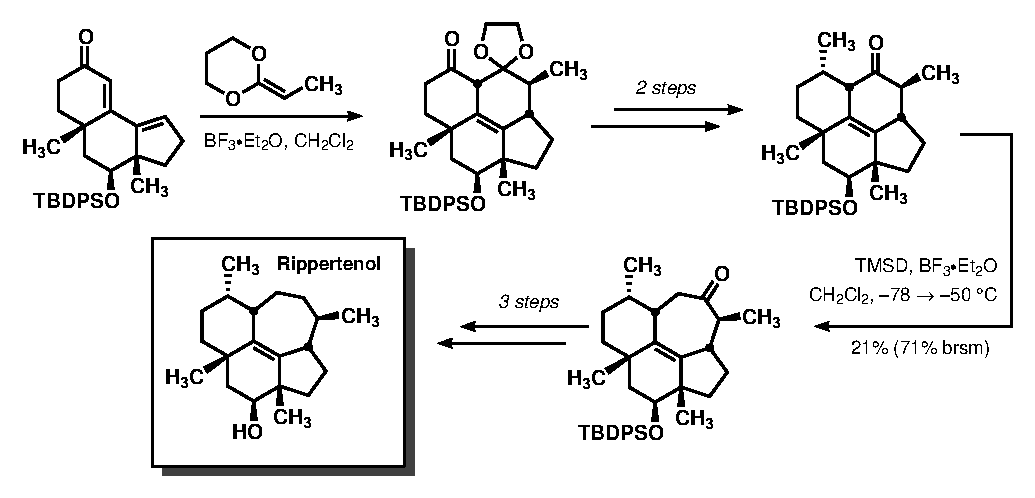
\includegraphics[scale=0.8]{chp_singlecarbon/images/snyder}
  \caption{Synder's total synthesis of rippertenol.}
\begin{textblock}{1}(2,-4.5) \cmp{bbn} \end{textblock}	
\begin{textblock}{1}(5.8,-7.8) \cmp{bbo} \end{textblock}	
\begin{textblock}{1}(10.6,-5.5) \cmp{bbp} \end{textblock}	
\begin{textblock}{1}(17.3,-5.5) \cmp{bbq} \end{textblock}	
\begin{textblock}{1}(14,-2) \cmp{bbr} \end{textblock}	
\begin{textblock}{1}(6.5,-1.5) \cmp{bbs} \end{textblock}	
  \label{sch:snyder}
\end{Scheme}


\clearpage
\section{Model Optimization Studies for Cyclopentanone Ring Expansions}
\label{sec:modeloptimization}

Previous studies from our group on scandium catalyzed single carbon ring expansion were focused
on $\alpha$-quaternary cyclobutanones,\crossref{ref:cdabrowski} and we were intent
on utilizing this methodology in the context of an advanced $\alpha$-quaternary substituted
cyclopentanone intermediate. We therefore chose to concentrate our
studies first on a suitable model system, 2-methyl-2-phenyl cyclopentanone (\ref{cmp:meph}), which
was prepared on gram scale by methods developed in our group for substituted carbon insertion.\footnote{See Chapter \ref{chp:asymmetric} for experimental details. \\
\includegraphics[scale=0.7]{chp_singlecarbon/images/meph}} 
\begin{table}[h] \centering
\vspace{10pt}
\includegraphics[scale=0.8]{chp_singlecarbon/images/comparisonhead}
\begin{textblock}{1}(5.5,-0.5) \cmp{meph}\end{textblock}
\begin{textblock}{1}(9.9,-0.5) \cmp{xbac} \end{textblock}
\begin{textblock}{1}(13.5,-0.5) \cmp{xbad} \end{textblock}
{\small
\begin{tabular}{ccccc}
\toprule 
entry$^a$ & promoter & conversion (\%) & yield \ref{cmp:xbac} (\%) & rr
(\ref{cmp:xbac}:\ref{cmp:xbad})
\\
\midrule
1$^b$&\ce{BF3.Et2O}&94& 80 & $>$100:1 \\
2$^c$&\ce{Al(CH3)3}&13& $<2$ & --  \\
\bottomrule
\multicolumn{5}{p{4.5in}}{\footnotesize $^a$Conversion, yield, and
regioselectivity were determined by GC analysis with hexamethylbenzene as an
internal standard. $^b$Run with 1.5 equivalents of \ce{BF3.Et2O} and TMSD.
$^c$Run with 1.2 equivalents of \ce{Al(CH3)3} and 1.1 equivalents TMSD.}
\end{tabular}
}
\caption{Establishing a point of comparison to previous methods.}
\label{tbl:comparison}
\end{table}
To establish a benchmark for our testing, we first evaluated the efficacy of the
Shioiri\crossref{ref:cshioiri} conditions (Table \ref{tbl:comparison}, entry 1).
We were surprised to see such high levels of regiocontrol with good yields of
the desired cyclohexanone \ref{cmp:xbac}. We then tested
Yamamoto's\crossref{ref:cyamamoto} conditions, which resulted in substantially
lower conversion and a poor yield of the desired product (entry 2). The Shioiri
conditions worked well in this context, but regardless required
superstoichiometric amounts of \ce{BF3.Et2O} to achieve high levels of
conversion. For this model substrate 1.5 equivalents was sufficient, but some
of the previously mentioned studies on more complex molecules required more than 4 equivalents. The
presence of Lewis basic functional groups other than the target ketone can interact with the Lewis
acid promoter and shut down the reaction. 

We then attempted to translate the previously reported conditions to our model
cyclopentanone substrate. Initial attempts resulted in highly irreproducible
reactions, rarely affording complete conversion. Even two identical reactions
run side by side under presumably the same conditions gave dramatically
different outcomes. Occasionally, reactions were successful, giving hope that
we could discover or control all the variables to produce a more reliable
reaction profile. We decided to approach the problem in two directions: (1) control all the
environmental variables by running with freshly purified reagents under dry conditions in a glove box, (2) monitor the reaction progress with an advanced analytical
technique to obtain the maximum possible information. 

Attempts to use ReactIR to monitor the reaction did not generate any usable data
and was operationally difficult to set up rigorously anhydrous reactions. ReactIR was abandoned
quickly in favor of $^1$H NMR spectroscopy, which proved to be operationally simpler and provided better
quality data. Reactions could be set up in a glove box and transferred to a J-Young tube
for analysis. In a glove box, rigorously vacuum dried \ce{Sc(OTf)3} was combined with cyclopentanone 
\ref{cmp:meph} in \ce{CDCl3} and allowed to stir for 15 minutes before adding 1.5 equivalents of
TMSD. The heterogeneous yellow reaction mixture was transferred to a J-Young NMR
tube, where a slow stream of nitrogen gas evolution began. $^1$H NMR data were recorded at
30 minute intervals and showed complete conversion after 450 minutes (7.5 hours)
at room temperature. After an additional 8 hours, no further
change was observed in the spectrum, and the mixture was then subjected to a dilute
acid hydrolysis. The products of the reaction were primarily
\ref{cmp:xbac} and \ref{cmp:xbad} in an 8:1 ratio by $^1$H NMR
spectroscopy. This promising result was promptly repeated with an identical
setup and gratifyingly afforded identical results. 

\begin{figure}[t]
  \centering
  \includegraphics[scale=0.55, trim = 45mm 45mm 30mm 40mm,
clip]{chp_singlecarbon/images/decompgraph}
  \caption{Decomposition of TMSD with \ce{Sc(OTf)3} and \ce{H2O}.}
  \begin{textblock}{3}(1,-9)  \begin{sideways}\small
  \textbf{\textsf{TMSD Remaining (\%)}} \end{sideways}
  \end{textblock}
\begin{textblock}{3}(8.5,-1.5)  \small \textbf{\textsf{Time (min)}}
\end{textblock}
\begin{textblock}{5}(10,-8)  \small \textsf{TMSD, \ce{Sc(OTf)3}, \ce{H2O} \\
t$_{\frac{1}{2}} = $ 19 minutes}
\end{textblock}
  \label{fig:decompgraph}
\end{figure}

With these two successful reactions, we still needed to determine the cause of
the previously irreproducible reactions. When the reactions were worked
up, they were first rinsed into a separatory funnel with benchtop \ce{Et2O}, which
immediately caused the rapid destruction of any remaining diazoalkane. We had
also observed that monitoring the reaction progress by thin layer chromatography
in certain cases also destroyed the diazoalkane. Trace amounts of water were
previously found to have a profound impact on both reaction kinetics and selectivity for asymmetric ring expansion reactions with chiral scandium catalysts.\footnote{\frenchspacing{Rendina, V. L.; Moebius, D. C.; Kingsbury, J. S. An Enantioselective Synthesis of 2-Aryl Cycloalkanones by Sc-Catalyzed Carbon Insertion. \textit{Org. Lett.}
\textbf{2011}, \textit{13}, 2004-2007.}} We rationalized that trace amounts of
water present in any of the reaction components, or adventitious atmospheric
water, may have been responsible for the inconsistent reactivity. An experiment was carried out to
test this hypothesis. When TMSD was mixed with 5 equivalents of water, an insignificant change in
the concentration\footnote{Determined by $^1$H NMR spectroscopy with
1,3,5-trimethoxybenzene as an internal standard.} was observed after 24
hours at room temperature. The same experiment with TMSD and 10 mol
\% \ce{Sc(OTf)3} also showed minimal change,\footnote{This result was
somewhat surprising given that Lewis acids are known to promote the
decomposition of diazoalkanes. See reference \ref{ref:cyamamoto}a and references
within.} but when an equivalent of water was added the diazoalkane began to
rapidly decompose (Figure \ref{fig:decompgraph}). In less than 20 minutes, half of the original
diazoalkane had been destroyed. The proposed pathway of decomposition is illustrated in Scheme
\ref{sch:scwatereq}.
Although \ce{Sc(OTf)3} is a water tolerant Lewis acid and is prepared from aqueous
triflic acid,\footnote{\frenchspacing{Kobayashi, S.; Hachiya, I.; Araki,
M.; Ishitani, H. Scandium Trifluoromethanesulfonate (Sc(OTf)$_3$). A Novel
Reusable Catalyst in the Diels-Alder Reaction. \textit{Tetrahedron Lett.}
\textbf{1993}, \textit{34}, 3755-3758.}} presumably an equilibrium can be
established with water which generates small quantities of acid.\footnote{{\frenchspacing Kobayashi,
S.; Nagayama, S.; Busujima, T.
Lewis Acid Catalysts Stable in Water. Correlation between Catalytic Activity in Water and Hydrolysis Constants and Exchange Rate
Constants for Substitution of Inner-Sphere Water Ligands. \textit{J. Am. Chem. Soc.} \textbf{1998},
\textit{120}, 8287-8288.}}  Br{\o}nsted acids
have long been known to facilitate rapid decomposition of diazoalkanes, first by
protonation and then by subsequent substitution with the conjugate base or an
appropriate nucleophile.\footnote{For a lead reference on the reaction of diazoalkanes with acids
see: {\frenchspacing Rendina, V. L.; Kingsbury, J. S. Titration of Nonstabilized Diazoalkane
Solutions by Fluorine NMR. \textit{J. Org. Chem.} \textbf{2012}, \textit{77}, 1181-1185.}} In this
case, water displaces nitrogen followed by a proton transfer to regenerate the Br{\o}nsted acid.
Trimethylsilyl methanol (\ref{cmp:bbt}) was not observed by $^1$H NMR
spectroscopy, instead a 1,2-Brook rearrangement\crossref{ref:cbrook} likely occurred to produce
methoxytrimethylsilane (\ce{->}\ref{cmp:bbu}). 
\begin{Scheme}[t]
  \centering \includegraphics[scale=0.8]{chp_singlecarbon/images/scwatereq}
  \caption{Proposed pathway for diazoalkane decomposition with hydrated
  scandium triflate.}
\begin{textblock}{1}(10,-0.1) \cmp{bbt} \end{textblock}
\begin{textblock}{1}(5,-0.1) \cmp{bbu} \end{textblock}		
  \label{sch:scwatereq}
\end{Scheme}


\begin{table}[t] \centering
\vspace{10pt}
\includegraphics[scale=0.8]{chp_singlecarbon/images/catscreenhead}
\begin{textblock}{1}(9.9,-0.5) \textsf{\scriptsize{\ref{cmp:xbac}}}
\end{textblock}
\begin{textblock}{1}(13.5,-0.5) \textsf{\scriptsize{\ref{cmp:xbad}}}
\end{textblock}
\begin{textblock}{1}(5.5,-0.5) \textsf{\scriptsize{\ref{cmp:meph}}}
\end{textblock}
{\small
\begin{tabular}{cccccc}
\toprule 
entry$^a$ & catalyst & time (h) & conversion (\%) & yield$^b$
(\%) & rr (\ref{cmp:xbac}:\ref{cmp:xbad})
\\
\midrule
\rowcolor{gray!15}1&\ce{Sc(OTf)3}&16&$>$98&88&7.4:1 \\
2&\ce{Sc(Cl)3(thf)3}&24&22&--&5.6:1 \\
3&\ce{Sc(hfac)3}&24&35&--&8:1 \\
4&\ce{ScBr3}&16&$<2$&--&-- \\
5&\ce{Sc(acac)3}&16&$<2$&--&-- \\
6&\ce{Y(OTf)3}&24&$<10$&--&-- \\
\rowcolor{gray!15}7&\ce{Yb(OTf)3}&24&80&70&55:1 \\
\bottomrule
\multicolumn{6}{p{5.1in}}{\footnotesize $^a$Conditions: 0.05
mmol scale, 10 mol \% catalyst, 2 equivalents TMSD, 0.1 M in
\ce{CH2Cl2}. Conversion, yield, and regioselectivity were determined by GC
analysis with hexamethylbenzene as an internal standard after treatment with 2
equivalents TBAF (1M in THF) and filtration through silica gel. $^b$Combined
yield of both regioisomers.}
\end{tabular}
}
\caption{Screen of Lewis acid catalysts.}
\label{tbl:catscreen}
\end{table}
With a reliable reaction protocol in hand, we began to evaluate other variables
to discover an optimized set of conditions. We first investigated other scandium
(III) salts and several other lanthanide triflates to ensure that we were
optimizing the best catalyst. Results of the catalyst screen are summarized in
\reftable{catscreen}. The highest yield of the major regioisomer
\ref{cmp:xbac} was obtained with \ce{Sc(OTf)3} (entry 1). Other less
Lewis acidic scandium salts (entries 2--5) resulted in lower levels of
conversion with comparable levels of regiocontrol. We were intrigued by the high
levels of regiocontrol observed with \ce{Yb(OTf)3} (entry 7). This less potent
and larger Lewis acid may enforce a more selective initial addition of the
diazoalkane, leading to the substantially higher regioselectivity. Later
attempts to use the stronger Lewis acid \ce{Yb(NTf2)3} to increase reaction
conversion resulted in rapid decomposition of the diazoalkane and low
conversion to the homologated products. We decided to continue optimizing
\ce{Sc(OTf)3} because of its higher activity and the ease that reactions could
be monitored by $^1$H NMR spectroscopy. Ytterbium (III) salts are paramagnetic
and complicated monitoring by NMR. 
\begin{table}[h] \centering
\vspace{10pt}
\includegraphics[scale=0.8]{chp_singlecarbon/images/solventscreenhead}
\begin{textblock}{1}(9.9,-0.5) \textsf{\scriptsize{\ref{cmp:xbac}}}
\end{textblock}
\begin{textblock}{1}(13.5,-0.5) \textsf{\scriptsize{\ref{cmp:xbad}}}
\end{textblock}
\begin{textblock}{1}(5.5,-0.5) \textsf{\scriptsize{\ref{cmp:meph}}}
\end{textblock}
{\small
\begin{tabular}{cccccc}
\toprule 
entry$^a$ & solvent & conversion (\%) & yield$^b$
(\%) & yield \ref{cmp:xbac}
(\%) & rr (\ref{cmp:xbac}:\ref{cmp:xbad})
\\
\midrule
1&\ce{CH2Cl2}&$>$98&88&78&7.4:1 \\
2&toluene&$>$98&95&79&5:1 \\
3&\ce{CHCl3}&$>$98&91&79&7:1 \\
4&\ce{hexanes}&94&86&75&6.8:1 \\
5&\ce{Et2O}&77&70&65&14.7:1 \\
6&\ce{THF}&27&10&8&3.2:1 \\
7&\ce{CH3CN}&62&28&25&8.2:1 \\
\bottomrule
\multicolumn{6}{p{5.1in}}{\footnotesize $^a$Conditions: 0.05
mmol scale, 10 mol \% \ce{Sc(OTf)3}, 2 equivalents TMSD, 0.1 M in solvent, 16 h.
Conversion, yield, and regioselectivity were determined by GC analysis with hexamethylbenzene as an internal standard after treatment with 2
equivalents TBAF (1M in THF) and filtration through silica gel. $^b$Combined
yield of both regioisomers.}
\end{tabular}
}
\caption{Solvent screen with \ce{Sc(OTf)3}.}
\label{tbl:solventscreen}
\end{table}

Table \ref{tbl:solventscreen} shows the results of a solvent screen with
catalytic \ce{Sc(OTf)3}. Entries 1--4 all showed high levels of conversion and
similar levels of regiocontrol, despite significant differences in polarity.
Even hexanes (entry 4), where the catalyst was completely heterogeneous,
proceeded to high conversion. Running in ethereal or Lewis basic solvents
(entries 5--7) not surprisingly supressed catalyst efficiency.\footnote{A similar observation was
made by Shioiri when using \ce{BF3.Et2O} as a promoter. Methylene chloride was selected as the
optimum solvent. See reference \ref{ref:cshioiri} for details.} The higher regiocontrol observed in
\ce{Et2O} suggested that filling the coordination sphere around scandium may produce a more selective catalyst. A single experiment examining regioselectivity as a function of conversion seemed to
indicate that binding of the product silyl enol ether resulted in higher
selectivity as the reaction progressed. The large discrepancy between conversion
and yield in \ce{CH3CN} (entry 7) was determined to be the result of
overhomologation to produce the cycloheptanone.


With a successful preliminary result (Table \ref{tbl:catscreen}, entry 1, page
\pageref{tbl:catscreen}), we still wanted to see if the yield of the major regioisomer could be
enhanced by increasing the regioisomeric ratio. We prepared the sterically more demanding
phenyldimethylsilyldiazomethane\footnote{\frenchspacing{Shioiri, T.;
Aoyama, T.; Mori, S. Trimethylsilyldiazomethane. \textit{Org. Synth.}
\textbf{1990}, \textit{68}, 1.} \label{ref:bshioriorgsynth}} (\ref{cmp:bbv}, \refscheme{pdmsd}) and
rationalized that higher levels of regioselectivity would be observed based on the preference for the
diazoalkane to add such that the bulky silicon group would be oriented away from
the more substituted side of the ketone. The intermediate \ref{cmp:bbw} avoids
this costly steric interaction and leads to the observed major regioisomer
\ref{cmp:xbac} in $>$15:1 selectivity, doubling the previously observed
selectivity with TMSD. For simpler model substrates, employing \ref{cmp:bbv} could provide
access to an easily isolable and synthetically useful more stable silyl enol ether with high
levels of regiocontrol.
\begin{Scheme}[t]
  \centering \includegraphics[scale=0.8]{chp_singlecarbon/images/pdmsd}
  \caption{Higher levels of regiocontrol with a more sterically hindered
  diazoalkane.}
\begin{textblock}{1}(5,-2) \cmp{bbv} \end{textblock}
\begin{textblock}{1}(12.2,-4) \cmp{bbw} \end{textblock}
\begin{textblock}{1}(11,-0.75) \cmp{bbx} \end{textblock}
\begin{textblock}{1}(2.25,-2) \textsf{\scriptsize{\ref{cmp:meph}}}
\end{textblock}
\begin{textblock}{1}(16.5,-4) \textsf{\scriptsize{\ref{cmp:xbac}}}
\end{textblock}
\begin{textblock}{1}(16.6,-0.75) \textsf{\scriptsize{\ref{cmp:xbad}}}
\end{textblock}
  \label{sch:pdmsd}
\end{Scheme}

Pleased with the performance of the \ce{Sc(OTf)3} TMSD system
thus far, we did not want to spend excessive time optimizing model substrate
\ref{cmp:meph}. Our synthetic strategy would ultimately involve homologation of
a \textit{cis}-fused 6,5-ring system (\refscheme{strategydecalin}, page
\pageref{sch:strategydecalin}), and we wanted to evaluate a more representative model. Commercially
available estrone 3-methyl ether (\ref{cmp:bby}) was subjected to two equivalents of TMSD and 5 mol \% \ce{Sc(OTf)3} in
deuterochloroform for 24 hours (\refscheme{estrone}). Complete
conversion and a 72\% yield of enol silane \ref{cmp:bbz} was observed by $^1$H NMR spectroscopy before deprotection
with TBAF. Purification by column chromatography afforded the major regioisomer
\ref{cmp:xbae} in an acceptable 68\% isolated yield along with 22\% of
\ref{cmp:xbaf}.
\begin{Scheme}[b]
  \centering 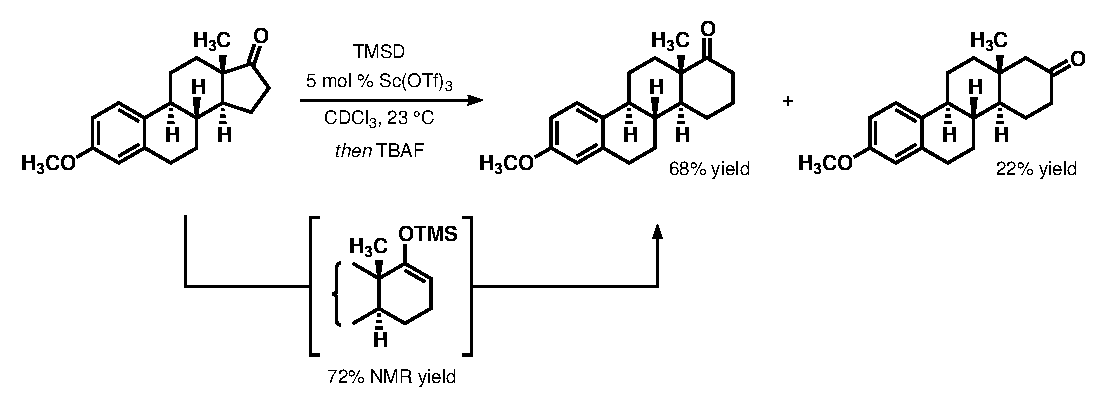
\includegraphics[scale=0.8]{chp_singlecarbon/images/estrone}
  \caption{Single carbon homologation of estrone 3-methyl ether.}
\begin{textblock}{1}(2.8,-3.6) \cmp{bby} \end{textblock}
\begin{textblock}{1}(7.2,-1) \cmp{bbz} \end{textblock}
\begin{textblock}{1}(11.4,-3.6) \cmp{xbae} \end{textblock}
\begin{textblock}{1}(16.5,-3.6) \cmp{xbaf} \end{textblock}
  \label{sch:estrone}
\end{Scheme}

With all of these results and information in hand, we were ready to start
looking at more complex substrates. The following section will discuss our
progress towards several sesquiterpene quinone natural products, with a focus on
the key ring expansion step. 

\clearpage
\section{Application to the Total Synthesis of 5-\textit{epi}-Ilimaquinone}


\begin{wrapfigure}{r}{1.7in}
  \vspace{-25pt}
  \begin{center}
    \includegraphics[scale=0.8]{chp_singlecarbon/images/5epiilimaquinone}
    \begin{textblock}{1}(2,-1) \cmp{bcf} \end{textblock}
  \end{center}
  \vspace{-30pt}
\end{wrapfigure}
We initially decided to concentrate our efforts on the synthesis of
5-\textit{epi}-ilimaquinone (\ref{cmp:bcf}), first isolated from the marine
sponge \textit{Fenestraspongia} by Faulkner and coworkers in
1985.\footnote{Originally isolated as a 2:3 mixture with
(--)-ilimaquinone. \frenchspacing{Cart\'e, B.; Rose, C. B.; Faulkner, D. J.
5-\textit{epi}-Ilimiquinone, a Metabolite of the Sponge \textit{Fenestraspongia} Sp.
\textit{J. Org. Chem.} \textbf{1985}, \textit{50}, 2785-2787.}} Access to
5-\textit{epi}-ilimaquinone, never prepared before by total synthesis, would
additionally faciliate access to several other related aminoquinone
derivatives. The section that follows
will discuss two synthetic generations, culminating in the successful
implementation of catalytic single carbon ring expansion through careful
experimentation and application of findings discussed in the previous section.

\subsection{First Generation Synthesis}
The retrosynthetic analysis for 5-\textit{epi}-ilimaquinone (\ref{cmp:bcf}) is
depicted in \refscheme{retrosynthesis}. We had also
originally planned to target several other natural aminoquinone derivatives
(\ref{cmp:bcc}, \ref{cmp:bcd}, \ref{cmp:bce}), which could theoretically be prepared in a single
substitution step from \ref{cmp:bcf} with the appropriate amine. A late-stage oxidation of aryl
intermediate \ref{cmp:bcg}, similar to that found in Snapper's synthesis of ($-$)-illimaquinone,
could provide the sensitive quinone moiety found in the final targets.\footnote{{\frenchspacing
Bruner, S. D.; Radeke, H. S.; Tallarico, J. A.; Snapper, M. L. Total Synthesis of (-)-Ilimaquinone.
\textit{J. Org. Chem.} \textbf{1995}, \textit{60}, 1114-1115.} \label{ref:csnapper}} Intermediate
\ref{cmp:bcg} could be accessed by olefination of \ref{cmp:bch}, which would be dervived from
\ref{cmp:xbas} following the key ring expansion event and hydrogenation to set the C-8
$\beta$-methyl stereocenter. Intermediate \ref{cmp:xbas} could be prepared from \ref{cmp:xban}
following olefination and oxidation steps. The pendant aryl group in \ref{cmp:xban} could be
attached by a dissolved metal reductive alyklation with reduced Hajos-Parrish ketone \ref{cmp:xbah} and aryl
iodide \ref{cmp:xbam}, introducing both the \textit{cis} ring junction and C-9 quaternary center.

\begin{Scheme}[t]
  \centering 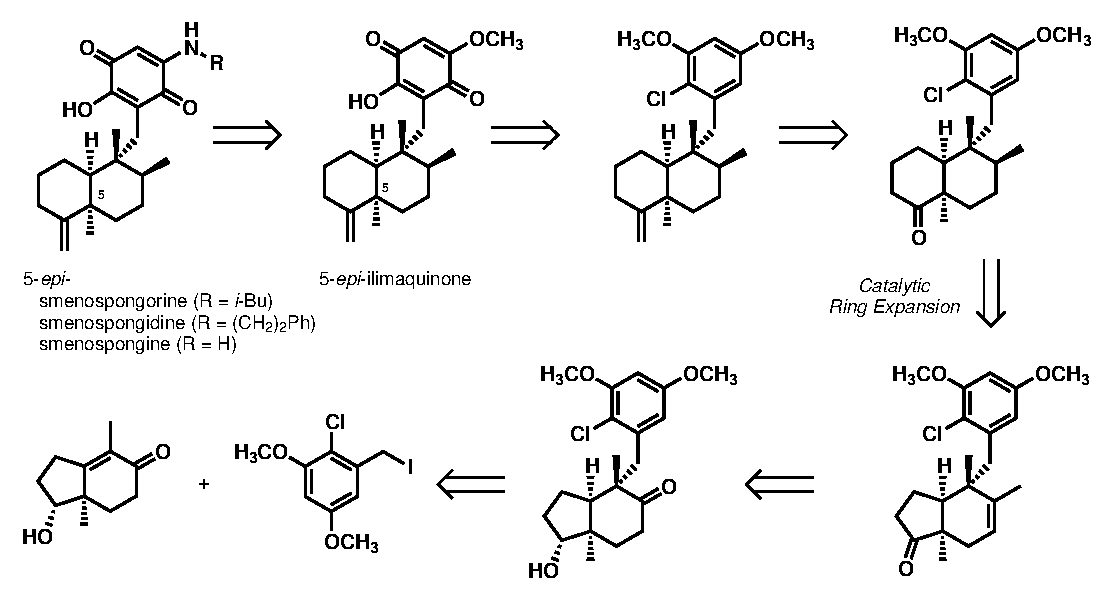
\includegraphics[scale=0.8]{chp_singlecarbon/images/retrosynthesis}
  \caption{Retrosynthetic analysis for 5-\textit{epi}-ilimaquinone and related
  aminoquinones.}
\begin{textblock}{1}(-0.3,-5.15) \cmp{bcc} \end{textblock}
\begin{textblock}{1}(-0.3,-4.75) \cmp{bcd} \end{textblock}
\begin{textblock}{1}(-0.3,-4.35) \cmp{bce} \end{textblock}
\begin{textblock}{1}(6.5,-6) \textsf{\scriptsize{\ref{cmp:bcf}}} \end{textblock}
\begin{textblock}{1}(11.6,-6) \cmp{bcg} \end{textblock}
\begin{textblock}{1}(17,-6.3) \cmp{bch} \end{textblock}
\begin{textblock}{1}(17,-0.2) \cmp{xbas} \end{textblock}
\begin{textblock}{1}(10.5,-0.2) \cmp{xban} \end{textblock}
\begin{textblock}{1}(4.5,-1)\cmp{xbam} \end{textblock}
\begin{textblock}{1}(1.4,-0.5) \cmp{xbah} \end{textblock}
  \label{sch:retrosynthesis}
\end{Scheme}

We began by preparing reduced Hajos-Parrish ketone \ref{cmp:xbah} according to a modified literature
protocol,\footnote{See the experimental section for details. {\frenchspacing Shigehisa, H.;
Mizutani, T.; Tosaki, S.; Ohshima, T.; Shibasaki, M. Formal Total Synthesis of (+)-Wortmannin Using
Catalytic Asymmetric Intramolecular Aldol Condensation Reaction. \textit{Tetrahedron} \textbf{2005},
\textit{61}, 5057-5065.}} which was obtained with $>$98\% ee after a single recrystallization.
Electrophile \ref{cmp:xbam} was selected because of its prior
use in the total synthesis of ($-$)-ilimaquinone by the Snapper
group.\footnote{The Snapper group utilized the corresponding aryl bromide. See reference
\ref{ref:csnapper} for details.} Starting from commercially available
3,5-dimethoxybenzoic acid (\ref{cmp:bcl}), reduction and chlorination afforded chloroalcohol \ref{cmp:xbak} (\refscheme{ephileone}). Standard bromination conditions allowed access to the benzyl bromide which was stable enough to be purified by silica gel chromatography. By employing
Finkelstein conditions, the more reactive benzyl iodide (\ref{cmp:xbam}) could be isolated cleanly
after simple filtration and concentration.

\begin{Scheme}[h]
  \centering
  \includegraphics[scale=0.8]{chp_singlecarbon/images/genoneelectrophile}
  \caption{First generation electrophile synthesis.}
  \begin{textblock}{1}(1.4,-0.75) \cmp{bcl} \end{textblock}
  \begin{textblock}{1}(8.5,-0.75)\cmp{xbak} \end{textblock}
  \begin{textblock}{1}(15.5,-0.75) \textsf{\scriptsize{\ref{cmp:xbam}}}
\end{textblock}
  \label{sch:ephileone}
\end{Scheme}


\begin{Scheme}[t]
  \centering
  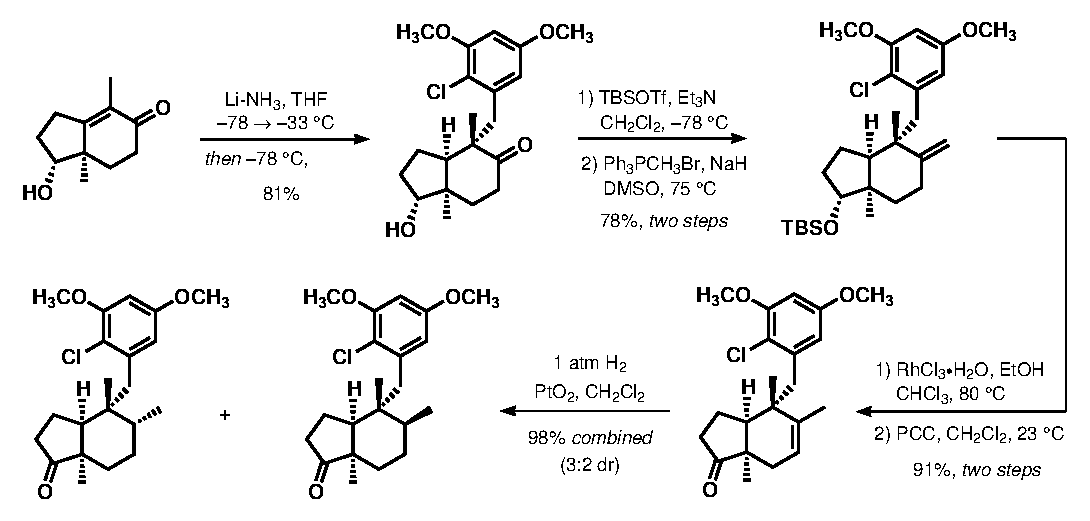
\includegraphics[scale=0.8]{chp_singlecarbon/images/forwardgenone}
  \caption{First generation forward synthesis.}
  \begin{textblock}{1}(16,-4.8) \cmp{xbaq} \end{textblock}
  \begin{textblock}{1}(6.4,0) \cmp{xbat} \end{textblock}
  \begin{textblock}{1}(1.5,0) \cmp{xbau} \end{textblock}
    \begin{textblock}{1}(13.5,0) \textsf{\scriptsize{\ref{cmp:xbas}}}
\end{textblock}
  \begin{textblock}{1}(8,-4.8) \textsf{\scriptsize{\ref{cmp:xban}}}
\end{textblock}
    \begin{textblock}{1}(1.6,-5.3) \textsf{\scriptsize{\ref{cmp:xbah}}}
\end{textblock}
  \begin{textblock}{1}(5.8,-6.3) \textsf{\scriptsize{\ref{cmp:xbam}}}
\end{textblock}
  \label{sch:forwardgenone}
\end{Scheme}
With fragments \ref{cmp:xbam} and \ref{cmp:xbah} in hand, we were prepared
to couple them in a single dissolved metal reductive alkylation step. In previous
examples, 6,6 ring systems were known to form exclusively \textit{trans} decalin
ring systems.\footnote{The stereochemical outcome of these reactions was extensively studied by
Stork. (a) {\frenchspacing Stork, G.; Darling, S. D. Stereochemistry of the Lithium-Ammonia
Reduction of $\alpha$,$\beta$-Unsaturated Ketones. \textit{J. Am. Chem. Soc.} \textbf{1960},
\textit{82}, 1512-1513.} (b) {\frenchspacing Stork, G.; Rosen, P.; Goldman, N. L. The
$\alpha$-Alkylation of Enolates From the Lithium-Ammonia Reduction of $\alpha$,$\beta$-Unsaturated
Ketones. \textit{J. Am. Chem. Soc.} \textbf{1961}, \textit{83}, 2965-2966.} (c) {\frenchspacing
Stork, G.; Darling, S. D. The Stereochemistry of the Lithium-Ammonia Reduction of
$\alpha$,$\beta$-Unsaturated Ketones. \textit{J. Am. Chem. Soc.} \textbf{1964}, \textit{86},
1761-1768.} (d) {\frenchspacing Stork, G.; Rosen, P.; Goldman, N.; Coombs, R. V; Tsuji, J.
Alkylation and Carbonation of Ketones by Trapping the Enolates from the Reduction of
$\alpha$,$\beta$-Unsaturated Ketones. \textit{J. Am. Chem. Soc.} \textbf{1965}, \textit{87},
275-286.}} Key to our synthetic strategy was the precedents for formation of a \textit{cis} ring
junction within the context of 6,5 ring systems.\footnote{Two examples are known in the literature:
(a) {\frenchspacing Paquette, L. A.; Wang, T.-Z.; Sivik, M. R. Total Synthesis of ($-$)-Austalide B.
A Generic Solution to Elaboration of the Pyran/p-Cresol/Butenolide Triad. \textit{J. Am. Chem. Soc.}
\textbf{1994}, \textit{116}, 11323-11334.} (b) {\frenchspacing Renoud-Grappin, M.; Vanucci, C.;
Lhommet, G. Diastereoselective Synthesis of a Limonoid Model Related to the Insect Antifeedant
Genudin. \textit{J. Org. Chem.} \textbf{1994}, \textit{59}, 3902-3905.}} However, previous examples
in the literature did not study the diastereoselectivity in these systems when trapping an
electrophile to form an all carbon quaternary center. Exposure of \ref{cmp:xbah} to lithium metal in ammonia formed a cup-shaped enolate intermediate after protonation at the ring fusion, facilitating a substrate controlled highly diastereoselective trap of electrophile \ref{cmp:xbam} (\ce{->} \ref{cmp:xban}, \refscheme{forwardgenone}). The \textit{cis} ring
fusion and stereochemistry of the newly forged all carbon quaternary center were later unambiguously
confirmed by X-ray crystallography.
Ketoalcohol \ref{cmp:xban} was protected\footnote{Olefination of unprotected \ref{cmp:xban} resulted
recovery of an unexpected product, likely the result of an intramolecular 1,5-hydride shift. See
section \ref{sec:hydride} (page \pageref{sec:hydride}) for further details.} and olefinated to
deliver \ref{cmp:xbaq} in 76\% yield over two steps. Attempts to hydrogenate \ref{cmp:xbaq}, the
free alcohol, or ketone to set the C-8 $\beta$-methyl stereocenter were less than satisfactory with
a variety of standard heterogeneous hydrogenation catalysts. We reasoned that moving the olefin into
the ring system and farther away from the congested C-9 quaternary center could favorably affect the
outcome of further hydrogenation efforts. Rhodium mediated isomerization\footnote{{\frenchspacing
Stahl, P.; Kissau, L.; Mazitschek, R.; Huwe, A.; Furet, P.; Giannis, A.; Waldmann, H. Total Synthesis and
Biological Evaluation of the Nakijiquinones. \textit{J. Am. Chem. Soc.} \textbf{2001}, \textit{123},
11586-11593.}} with concomitant silyl deprotection followed by PCC oxidation provided cyclopentanone
\ref{cmp:xbas} in a 91\% yield over two steps.
Hydrogenation over Adams' catalyst delivered epimeric cyclopentanones \ref{cmp:xbat} and
\ref{cmp:xbau} in an unoptimized 3:2 dr slightly favoring the desired $\beta$-methyl epimer. We
turned our attention next to the key ring expansion event with two potential cyclopentanone
substrates in hand (\ref{cmp:xbas} and \ref{cmp:xbat}).

\begin{Scheme}[b]
  \centering
  \includegraphics[scale=0.8]{chp_singlecarbon/images/homoone}
    \begin{textblock}{1}(12.2,-0.5) \cmp{xbav} \end{textblock}
    \begin{textblock}{1}(5,-0.5) \textsf{\scriptsize{\ref{cmp:xbas}}}
\end{textblock}
  \caption{Successful ring expansion of cyclopentanone \ref{cmp:xbas}.}
  \label{sch:homoone}
\end{Scheme}
We were pleased to see that the conditions optimized previously for model
systems translated exceptionally well to cyclopentanone \ref{cmp:xbas} with very
little modification (\refscheme{homoone}). Exposure of \ref{cmp:xbas} to 10 mol \%
\ce{Sc(OTf)3} and 1.5 equivalents of TMSD in \ce{CDCl3} showed only 33\% conversion after 18
hours at room temperature. Simply heating the reaction mixture to 50
\degc~resulted in 88\% conversion in an additional 9 hours and complete
conversion with a further 10 hours of heating. After dilute acid hydrolysis, the
regioselectivity by $^1$H NMR spectroscopy was approximately 6:1,
favoring the desired regioisomer (\ref{cmp:xbav}). Dropping the catalyst loading to 5 mol \% and
increasing the concentration allowed the desired cyclohexanone to be recovered
in an 89\% isolated yield ($>$8:1 regioselectivity, 16 h, 50 \degc) after protodesilylation. We also
attempted to use the bulkier PDMSD with \ref{cmp:xbas}, which had previously performed better in the context of model studies (\refscheme{pdmsd}, page
\pageref{sch:pdmsd}). After heating for 24 hours at 50 \degc\  the reaction mixture was analyzed by
$^1$H NMR spectroscopy and showed a single regioisomer; however, the conversion had only reached
75\% during this time period (\ce{->} \ref{cmp:xbav}, \refscheme{homoonepdms}). The larger
diazoalkane afforded the higher levels of regioselectivity expected from model studies, but the
reaction efficiency suffered. Content with the use of TMSD, we attempted to press forward with
\ref{cmp:xbav} in hand. Unfortunately, all attempts to hydrogenate \ref{cmp:xbav} were
unsucessful.\footnote{A complete discussion of attempts to further transform \ref{cmp:xbav} and
related compounds will be included as part of the Ph.D. dissertation of Hilan Z. Kaplan.
\label{ref:kaplancopout}} \begin{Scheme}[h]
  \centering
  \includegraphics[scale=0.8]{chp_singlecarbon/images/homoonepdms}
    \begin{textblock}{1}(12.2,-0.5) \textsf{\scriptsize{\ref{cmp:xbav}}} \end{textblock}
    \begin{textblock}{1}(5,-0.5) \textsf{\scriptsize{\ref{cmp:xbas}}}
\end{textblock}
  \caption{Higher regiocontrol but lower efficiency with PDMSD.}
  \label{sch:homoonepdms}
\end{Scheme}


\begin{Scheme}[t]
  \centering
  \includegraphics[scale=0.8]{chp_singlecarbon/images/homoonebeta}
   \begin{textblock}{1}(12.6,-0.5) \cmp{bcm} \end{textblock}
    \begin{textblock}{1}(5,-0.5) \textsf{\scriptsize{\ref{cmp:xbat}}}
\end{textblock}
  \caption{Complete decomposition with forcing conditions.}
  \label{sch:homoonebeta}
\end{Scheme}
When $\beta$-methyl cyclopentanone \ref{cmp:xbat} was subjected to similar homologation
conditions optimized above for \ref{cmp:xbas} (5 mol \% \ce{Sc(OTf)3}, 2 equivalents TMSD), we were
disappointed to see a complete lack of reactivity. Heating the reaction mixture to 50 \degc\ did nothing to drive a productive reaction,
instead simply accelerated decomposition of the diazoalkane. The starting cyclopentanone was
returned unchanged. In another experiment with 6 equivalents of TMSD, heating to 70 \degc\ lead to
complete decomposition of the diazoalkane and starting material (\refscheme{homoonebeta}). Not even
a trace amount of the characteristic enol silane \ref{cmp:bcm} could be detected. A control
experiment containing a mixture of $\beta$-- and $\alpha$-methyl cyclopentanones \ref{cmp:xbat} and \ref{cmp:xbau} was run with two equivalents of TMSD and 5 mol \% \ce{Sc(OTf)3} at 50 \degc\ 
overnight. We were able to observe complete conversion of the $\alpha$ epimer \ref{cmp:xbau} by
$^1$H NMR, but the $\beta$ epimer remained completely untouched. This control indicated that our
reaction was working properly and something particular about the $\beta$ epimer was preventing the
homologation reaction from occuring. 

\begin{figure}[h]
  \centering
  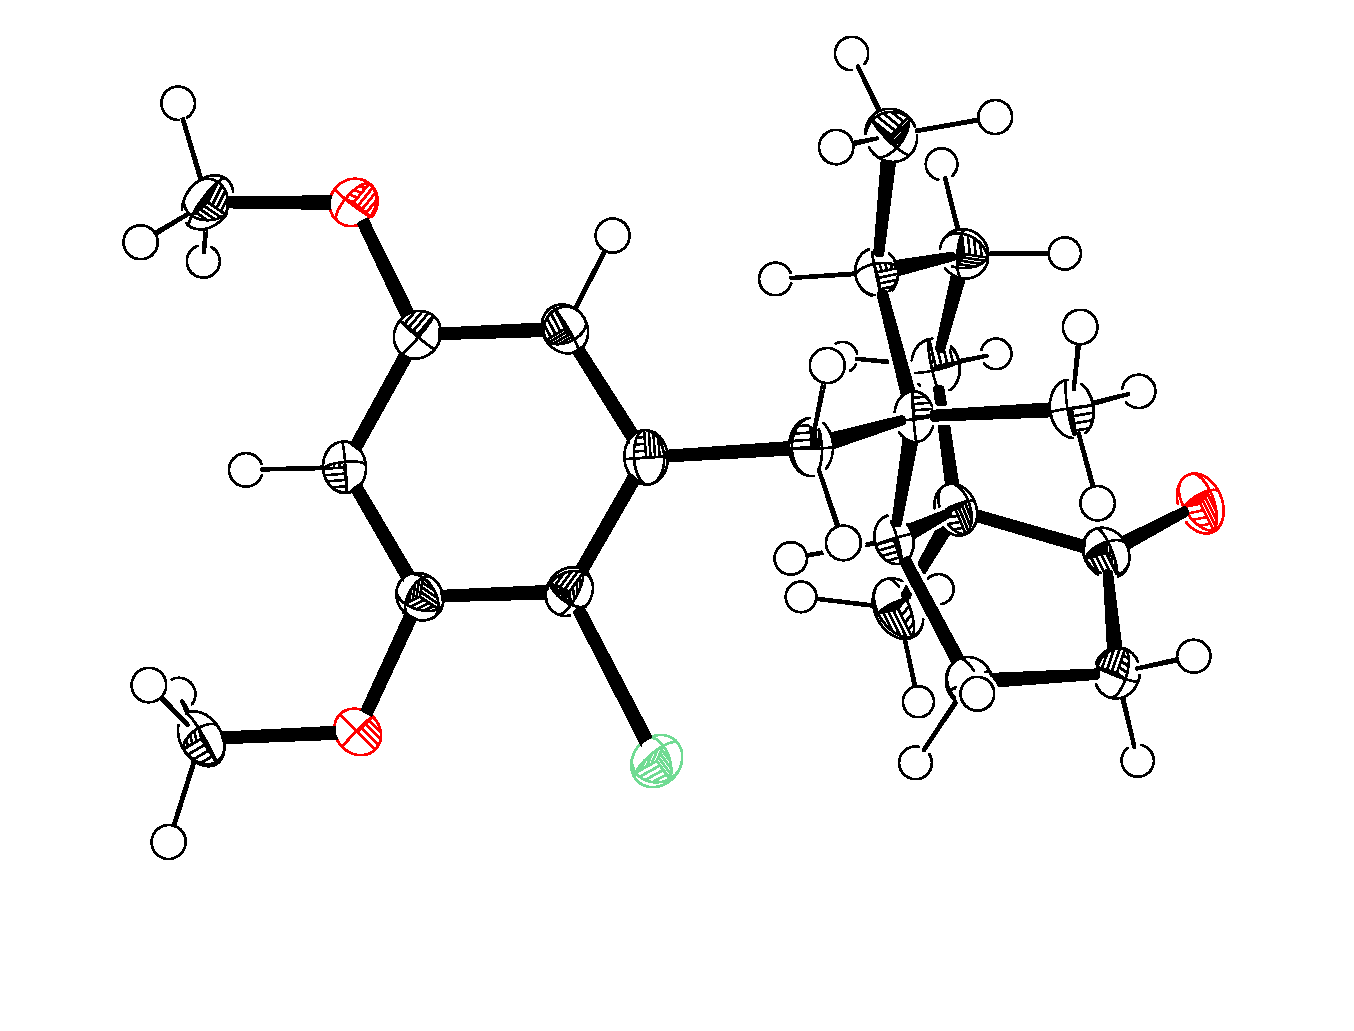
\includegraphics[scale=0.4, trim = 10mm 0mm 15mm -125mm,
clip,
  angle=92]{chp_singlecarbon/images/betamethylcrystal}
    \begin{textblock}{1}(3.3,-10) \textsf{\scriptsize{\ref{cmp:xbat}}} \end{textblock}
   \begin{textblock}{1}(3,-10)
  \includegraphics[scale=0.8]{chp_singlecarbon/images/betamethylstructure}
  \end{textblock}
  \caption{ORTEP diagram of $\beta$-methyl hydrogenation product.}
  \label{fig:betamethylcrystal}
\end{figure}
Looking at the solid state structure of $\beta$-methyl cyclopentanone \ref{cmp:xbat} revealed a
likely rationale for why this substrate failed to undergo homologation even under strongly forcing
conditions (\reffigure{betamethylcrystal}). Access to the $\pi$* orbital of the carbonyl was
exceptionally hindered by angular methyl groups on both sides of the molecule. The $\alpha$ face of the carbonyl was
effectively blocked by the adjacent methyl group and the $\beta$ face was shielded by the axial
methyl group on the C-9 quaternary center. The solid state structure of the $\alpha$-methyl
cyclopentanone \ref{cmp:xbau} revealed a different chair conformation where the $\beta$ face of the
carbonyl was now more accessible (\reffigure{alphamethylcrystal}).  Although the solid state structure may not
accurately represent the solution phase structure as there may be more conformational liberty in
solution, these structural features shed light on why \ref{cmp:xbau} readily underwent
homologation, whereas \ref{cmp:xbat} was completely inert.
 \begin{figure}[h]
  \centering
  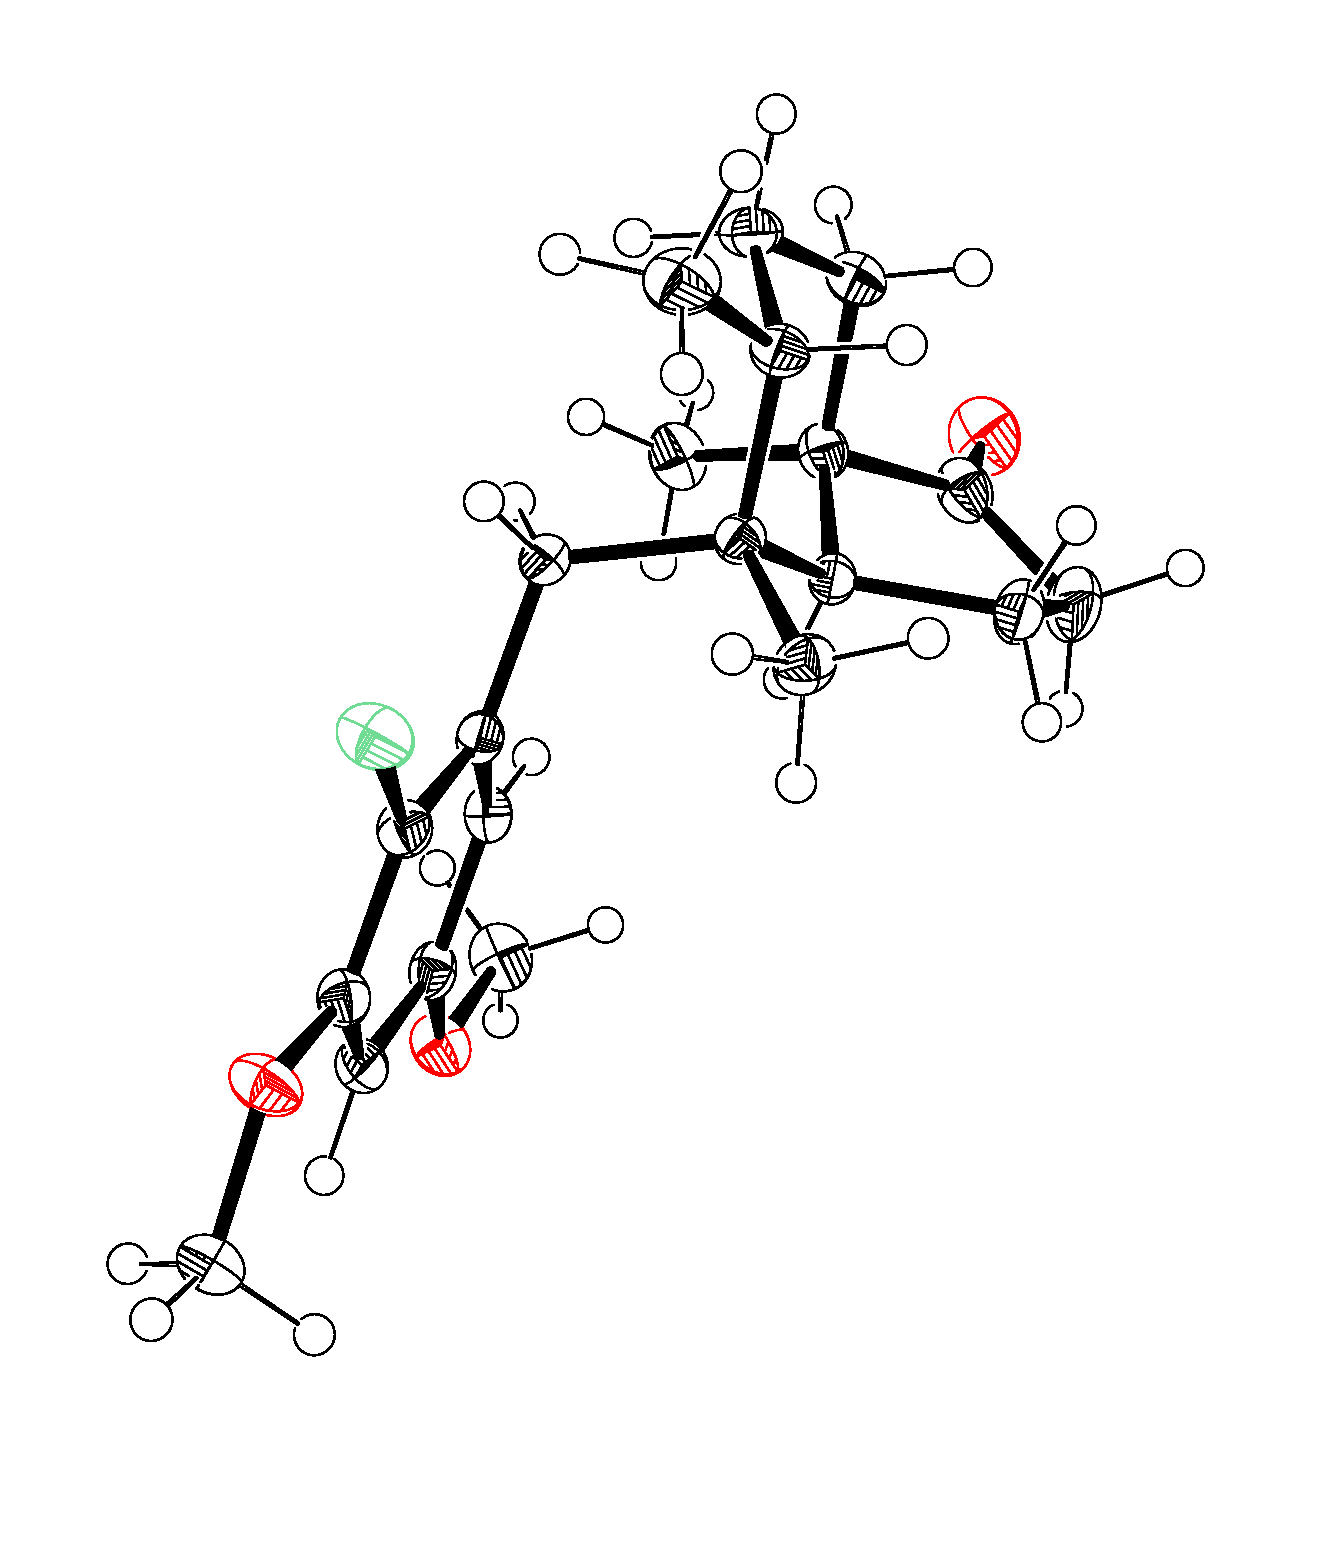
\includegraphics[scale=0.40, trim = 10mm -50mm 15mm 0mm,
clip,
  angle=92]{chp_singlecarbon/images/alphamethylcrystal}
  \begin{textblock}{1}(12,-10)
  \includegraphics[scale=0.8]{chp_singlecarbon/images/alphamethylstructure}
  \end{textblock}
   \begin{textblock}{1}(13,-10) \textsf{\scriptsize{\ref{cmp:xbau}}} \end{textblock}
  \caption{ORTEP diagram of $\alpha$-methyl hydrogenation product.}
  \label{fig:alphamethylcrystal}
\end{figure}


\subsection{Second Generation Synthesis}

The first generation dissolved metal reductive alkylation (\ref{cmp:xbah} + \ref{cmp:xbam} \ce{->}
\ref{cmp:xban}, \refscheme{forwardgenone}, page \pageref{sch:forwardgenone}) and subsequent single
carbon homologation reactions with trisubstituted ene-one \ref{cmp:xbas} performed exceptionally
well. However, we ran into a number of unexpected difficulties when attempting to further transform
cyclohexanone \ref{cmp:xbav}. Installing the C-8 $\beta$-methyl stereogenic
center appeared to be an insurmountable problem.\crossref{ref:kaplancopout} In an attempt to address
these issues, a second generation route was designed. The synthetic strategy remained largely the
same for the second generation route. A dissolved metal reductive alkylation event would build a significant portion of the carbon framework and set the key
\textit{cis} ring fusion. Ring expansion with TMSD would then provide access to the decalin core
found in the final target. The major difference in the second generation was the selection of
electrophile.

\begin{Scheme}[b]
  \centering
  \includegraphics[scale=0.8]{chp_singlecarbon/images/gentwoelectrophile}
  \begin{textblock}{1}(2.2,0) \cmp{bcn} \end{textblock}
  \begin{textblock}{1}(8.8,0) \cmp{xbaw} \end{textblock}
  \begin{textblock}{1}(15.5,0) \cmp{xbay} \end{textblock}
  \caption{Second generation electrophile synthesis.}
  \label{sch:ephiletwo}
\end{Scheme}
We wanted to incorporate functionality into the electrophile that could be unmasked later and
provide a means to direct a homogeneous hydrogenation catalyst to the $\beta$-face of the
molecule.\footnote{{\frenchspacing Hoveyda, A.
H.; Evans, D.
A.; Fu, G.
C.
Substrate-Directable Chemical Reactions. \textit{Chem. Rev.} \textbf{1993}, \textit{93},
1307-1370.}} A similar directed hydrogenation strategy was employed by Terashima to set the C-8
methyl stereogenic center in his synthesis of ($+$)-arenarol, a natural product containing a very
similar \textit{cis}-decalin carbon framework.\footnote{{\frenchspacing Kawano, H.; Masanori, I.;
Tadashi, K.; Terashima, S. Studies Toward the Synthesis of Popolohuanone E: Synthesis of Natural
(+)-Arenarol Related to the Proposed Biogenetic Precursor of Popolohuanone E.
\textit{Tetrahedron Lett.} \textbf{1997}, \textit{38}, 7769-7772.}} We began by preparing
electrophile \ref{cmp:xbay} (\refscheme{ephiletwo}), which contained an orthogonally protected
phenol that we planned to use later as a directing group and ultimately as a functional handle for
quinone oxidation.\footnote{Early model studies on the oxidation of free phenols with Fremy's salt
were very promising. {\frenchspacing Wehrli, P.
A.; Pigott, F.
Oxidation with the Nitrosodisulfonate Radical. I. Preparation and Use of Disodium
Nitrosodisulfonate: Trimethyl-\textit{p}-Benzoquinone.
\textit{Org. Synth.} \textbf{1972}, \textit{52}, 83.} For a review see: {\frenchspacing Zimmer, H.;
Lankin, D. C.; Horgan, S. W. Oxidations with Potassium Nitrosodisulfonate (Fremy's Radical). The
Teuber Reaction. \textit{Chem. Rev.} \textbf{1971}, \textit{72}, 229-246.}} Starting from benzyl
alcohol \ref{cmp:bcn}, regioselective chlorination with 1,3-dichloro-5,5-dimethylhydantoin delivered
the desired aryl-chloride \ref{cmp:xbaw} in 92\% yield.\footnote{{\frenchspacing Auerbach, J.;
Weissman, S. A.; Blacklock, T. J.; Angeles, M. R.; Hoogsteen, K.
\textit{N}-Bromosuccinimide / Dibromodimethylhydantoin in Aqueous Base: A Practical Method for the
Bromination of Activated Benzoic Acids. \textit{Tetrahedron Lett.} \textbf{1993}, \textit{34},
931-934.}} Bromination under Appel conditions,\footnote{{\frenchspacing Appel, R. Tertiary
Phosphane/Tetrachloromethane, a Versatile Reagent for Chlorination, Dehydration, and P--N Linkage.
\textit{Angew. Chem. Int. Ed.} \textbf{1975}, \textit{14}, 801-811.}} followed by displacement of
the bromide with sodium iodide provided decagram-scale access to the desired second generation
electrophile \ref{cmp:xbay} in an 86\% yield over two steps.

\begin{Scheme}[h]
  \centering \includegraphics[scale=0.8]{chp_singlecarbon/images/forwardgentwo}
  \begin{textblock}{1}(8.5,0) \cmp{xbaz} \end{textblock}
  \begin{textblock}{1}(15.5,0) \cmp{xbbc} \end{textblock}
 \begin{textblock}{1}(2.4,-0.5) \textsf{\scriptsize{\ref{cmp:xbah}}} \end{textblock}
 \begin{textblock}{1}(6.5,-1.62) \textsf{\scriptsize{\ref{cmp:xbay}}} \end{textblock}
  \caption{Second generation forward synthesis.}
  \label{sch:forwardgentwo}
\end{Scheme}
\begin{Scheme}[b]
  \centering \includegraphics[scale=0.8]{chp_singlecarbon/images/forwardgentwodiverge}
  \begin{textblock}{1}(1.4,0) \cmp{xbbe} \end{textblock}
  \begin{textblock}{1}(16.5,0) \cmp{xbbg} \end{textblock}
 % \begin{textblock}{1}(15.5,0) \cmp{xbay} \end{textblock}
 \begin{textblock}{1}(9,0) \textsf{\scriptsize{\ref{cmp:xbbc}}} \end{textblock}
  \caption{Divergent approach in second generation synthesis.}
  \label{sch:forwardgentwodiverge}
\end{Scheme}
We then proceeded with the dissolved metal reductive alkylation of
electrophile \ref{cmp:xbay} and reduced Hajos-Parrish ketone \ref{cmp:xbah}. The reductive
alkylation smoothly delivered the desired keto-alcohol \ref{cmp:xbaz} in 79\% yield after column
chromatography (\refscheme{forwardgentwo}). Silyl protection under standard conditions and
Wittig olefination afforded \ref{cmp:xbbc} in 85\% yield over two steps. At this stage in the
previous generation synthesis we isomerized the 1,1-disubstituted exocyclic olefin to help
facilitate a poorly diastereoselective hydrogenation over Adam's catalyst (\refscheme{forwardgenone}, page
\pageref{sch:forwardgenone}). By diverging the material at this point and
bringing forward both the 1,1-disubstituted olefin and the trisubstituted olefin, we could have
more substrates to test in the homologation reaction and subsequent hydrogenation
(\refscheme{forwardgentwodiverge}).
Direct deprotection of \ref{cmp:xbbc} with TBAF followed by Dess-Martin oxidation provided access to
the exocyclic 1,1-disubstituted cyclopentanone \ref{cmp:xbbe} in quantitative yield over two steps.
Rhodium mediated isomerization and deprotection of \ref{cmp:xbbc} followed by Dess-Martin oxidation
afforded the trisubtituted olefin \ref{cmp:xbbg} in 98\% yield over two steps. Attempts were not
made to hydrogenate either \ref{cmp:xbbe} or \ref{cmp:xbbg} prior to the homologation event because
of our previous challenges with $\beta$-methyl cyclopentanone \ref{cmp:xbat}.

\begin{Scheme}[h]
  \centering 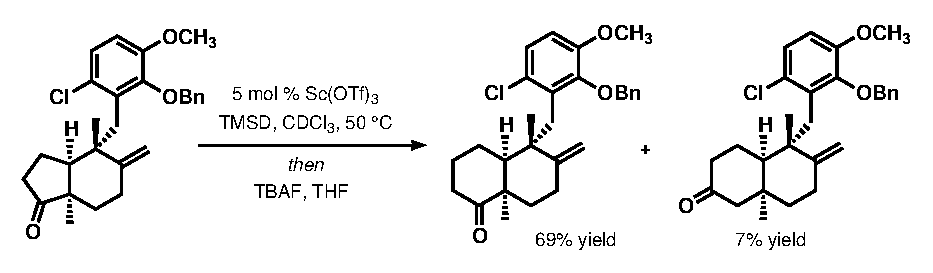
\includegraphics[scale=0.8]{chp_singlecarbon/images/homotwoexocyclic}
 \begin{textblock}{1}(12,-1.5) \cmp{xbbh} \end{textblock}
 \begin{textblock}{1}(17,-1.5) \cmp{xbbi} \end{textblock}
\begin{textblock}{1}(3,-0.5) \textsf{\scriptsize{\ref{cmp:xbbe}}} \end{textblock}
  \caption{Homologation of \ref{cmp:xbbe} gives diminished selectivity and yields.}
  \label{sch:homotwoexocyclic}
\end{Scheme}
\begin{Scheme}[b]
  \centering 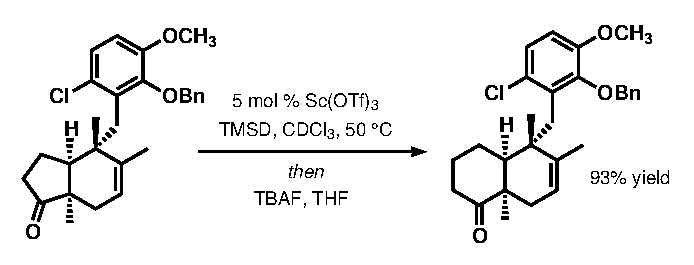
\includegraphics[scale=0.8]{chp_singlecarbon/images/homotwotrisub}
 \begin{textblock}{1}(13,-0.25) \cmp{xbbj} \end{textblock}
 \begin{textblock}{1}(5,-0.25) \textsf{\scriptsize{\ref{cmp:xbbg}}} \end{textblock}
  \caption{Excellent yield with the homologation of \ref{cmp:xbbg}.}
  \label{sch:homotwotrisub}
\end{Scheme}
We then focused on the key ring expansion event with two additional cyclopentanone substrates in
hand (\ref{cmp:xbbe}, \ref{cmp:xbbg}). We were pleased again to see that both substrates readily
underwent homologation with mild warming of the reaction mixture, reaching full conversion in less
than 24 hours.
Exocyclic cyclopentanone \ref{cmp:xbbe} delivered a slightly diminished 69\% isolated yield of the desired major regioisomer
\ref{cmp:xbbh}, along with a 7\% isolated yield of the minor regioisomer \ref{cmp:xbbi}
(\refscheme{homotwoexocyclic}, approx.
7:1 rr by crude $^1$H NMR).
Isomerized cyclopentanone \ref{cmp:xbbg} afforded an excellent 93\% isolated yield of the target
homologated product \ref{cmp:xbbj} (\refscheme{homotwotrisub}). The homologation reaction of
\ref{cmp:xbbg} tracked well with the results obtained in the first generation route with \ref{cmp:xbas} (89\% isolated, $>$8:1 rr). These results
illustrate how seemingly subtle changes to the molecule can have a fairly striking effect on the
outcome of the homologation reaction. 
 
 \begin{figure}[h]
  \centering
  \vspace{-60pt}
  \includegraphics[scale=0.30]{chp_singlecarbon/images/homotwomodel}
  \vspace{-75pt}
   \begin{textblock}{1}(13,-9) \textsf{\scriptsize{\ref{cmp:xbbe}}} \end{textblock}
   \begin{textblock}{1}(1,-9) \textsf{\scriptsize{\ref{cmp:xbbg}}} \end{textblock}
  \caption{Modeling of cyclopentanones \ref{cmp:xbbe} and \ref{cmp:xbbg} reveals different chair 
  conformations.}
  \label{fig:homotwomodel}
\end{figure}
Modeling of cyclopentanones \ref{cmp:xbbe} and \ref{cmp:xbbg} \textit{in silico} revealed that the
position of the olefin significantly impacts the preferred chair conformation of the
molecule.\footnote{Optimized geometries were calculated with Gaussian '09 - B3LYP 3-21G / Avogadro
1.03} The endocyclic olefin cyclopentanone \ref{cmp:xbbg} (left, \reffigure{homotwomodel}) adopts a
half-chair conformation that places both the C-9 appended aryl group and $\alpha$-keto methyl in a
distorted 1,3-diaxial orientation. The exocyclic olefin cyclopentanone \ref{cmp:xbbe} (right,
\reffigure{homotwomodel}) prefers a twist-boat conformation where the C-9 aryl moiety rests in an
equatorial disposition and the $\alpha$-keto methyl remains axial. The change in conformation
translates to a modified steric environment around the ketone, which in turn affects the outcome
of the homologation reactions. 



The homologation reactions performed exceptionally well, and we were especially pleased to see that
reactions worked consistently. The reliability and scalability of the reaction allowed ample
quantities of material to be moved forward. Again significant hardships were encountered when
attempting to further transform both
\ref{cmp:xbbh} and \ref{cmp:xbbj}. A complete discussion is beyond the scope of this chapter and will be discussed elsewhere.\crossref{ref:kaplancopout}


\subsection{An Unexpected 1,5-Hydride Shift}
\label{sec:hydride}

\begin{Scheme}[b]
  \centering
  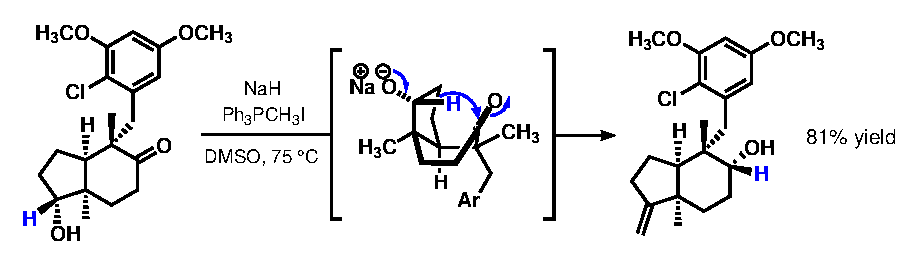
\includegraphics[scale=0.8]{chp_singlecarbon/images/hydrideone}
  \begin{textblock}{1}(3.8,-0.25) \textsf{\scriptsize{\ref{cmp:xban}}} \end{textblock}
  \begin{textblock}{1}(8.5,-0.6) \cmp{bco}  \end{textblock}
  \begin{textblock}{1}(14,-0.25) \cmp{xbao}  \end{textblock}
  \caption{Unexpected molecular rearrangement during Wittig olefination.}
  \label{sch:hydrideone}
\end{Scheme}
During the course of our studies we observed an unexpected molecular rearrangement when attempting
to directly olefinate the \textit{cis}-fused keto alcohol products derived from
dissolved metal reductive alkylation.
When keto-alcohol \ref{cmp:xban} was subjected to Wittig methylenation conditions, an ene-carbinol
isomeric with the anticipated product was isolated in an 81\% yield
(\ce{->}\ref{cmp:xbao}, \refscheme{hydrideone}).
The observed product, whose connectivity was rigorously established by TOCSY NMR data, was the result of what we believed to be
a transannular 1,5-hydride migration followed by cyclo\textit{pentanone} methylenation. This type of
internal redox event has been observed previously in a number conformationally biased bicyclic
systems.\footnote{(a) {\frenchspacing Dvornik, D.; Edwards, O. E. Ajaconine: An Intramolecular
Cannizzaro-type Reaction and the Location of the Undefined Oxygen. \textit{Proc. Chem. Soc.}
\textbf{1958}, 280-281.} (b) {\frenchspacing Acklin, W.; Prelog, V. Die Bestimmung der absoluten
Konfiguration von 8-Methyl-hydrindan-Derivaten durch asymmetrische Synthese. Eine intramolekulare
1,5-Hydrid-Verschiebung in der \textit{cis}-Hydrindan-Reihe. \textit{Helv. Chim. Acta.}
\textbf{1959}, \textit{42}, 1239-1247.} (c) {\frenchspacing Parker, W.; Stevenson, J. R. A
Transannular 2,6-Hydride Shift in the Bicyclo[3,3,1]nonane System. \textit{J. Chem. Soc. Chem.
Comm.} \textbf{1969}, 1289-1290.} (d) {\frenchspacing Wicha, J.; Caspi, E. Transformations of
Steroidal Neopentyl Systems. VII. Mechanism of the Transformation of
(19\textit{R})-Hydroxy-19a-methyl-(5$\alpha$)-3-ones to
19-Keto-19a-methyl-(5$\alpha$)-3$\alpha$-hydroxy Analogs. \textit{J. Org. Chem.} \textbf{1973},
\textit{38}, 1280-1283.} (e) {\frenchspacing Shepherd, J. M.; Singh, D.; Wilder Jr., P. An Alkali
Induced 1,4-Hydride Shift in endo-Tricyclo[5.2.1.0]decyl Ketols. \textit{Tetrahedron Lett.}
\textbf{1974}, \textit{15}, 2743-2746.} (f) {\frenchspacing Warnhoff, E. W. A Base-induced
Transannular 1,4-Hydride Shift in a Cyclohexanone. \textit{J. Chem. Soc. Chem. Comm.} \textbf{1976},
517-518.} \label{ref:hydriderefs}} We speculated that the two quaternary carbon centers, arranged
1,3 around the cyclohexanone, would suffer from a 1,3-diaxial interaction in either chair conformer. Under the
reaction conditions, a boat conformation (\ref{cmp:bco}) that helps alleviate some of the penalizing
1,3 interactions could be energetically accessible and allow the migrating hydrogen to come in close
proximity of the carbonyl $\pi$* orbital. In the second generation synthesis we also observed a similar molecular rearrangement with
unprotected keto-alcohol \ref{cmp:xbaz} (\refscheme{hydridetwo}). Instead of isolating the analogous 
rearranged ene-carbinol, further transformation of \ref{cmp:bcp} led to the unusual tetracyclic
olefin \ref{cmp:xbba} which could be recovered in a 60\% isolated yield. All analytical data were
consistent with structure \ref{cmp:xbba} and no other major products were isolated from the reaction
mixture.
\begin{Scheme}[t]
  \centering
  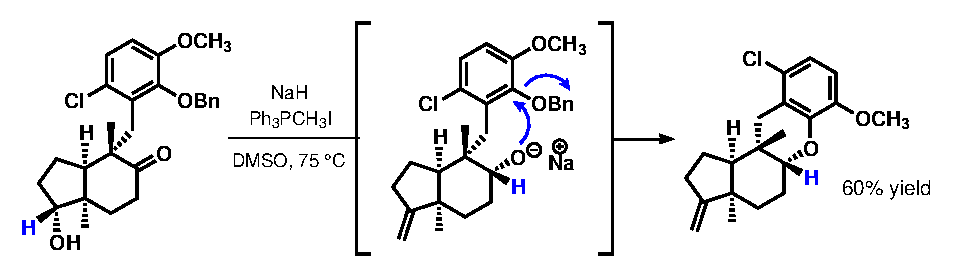
\includegraphics[scale=0.8]{chp_singlecarbon/images/hydridetwo}
  \begin{textblock}{1}(3.4,-0.25) \textsf{\scriptsize{\ref{cmp:xbaz}}} \end{textblock}
  \begin{textblock}{1}(10.5,-0.6) \cmp{bcp}  \end{textblock}
  \begin{textblock}{1}(14.5,-0.25) \cmp{xbba}  \end{textblock}
  \caption{Further molecular rearrangement with second generation electrophile.}
  \label{sch:hydridetwo}
\end{Scheme}
\begin{Scheme}[hb]
  \centering
  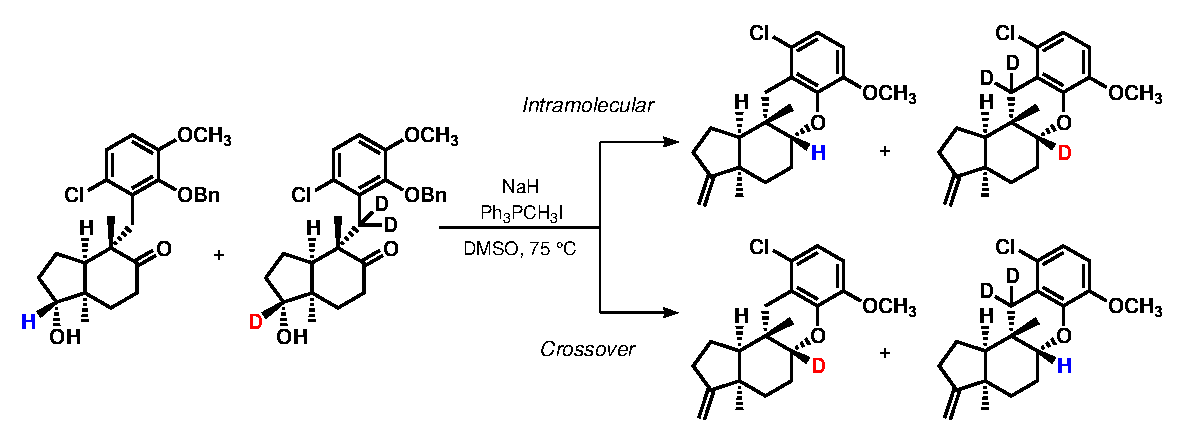
\includegraphics[scale=0.8]{chp_singlecarbon/images/crossover}
  \begin{textblock}{1}(1,-1) \textsf{\scriptsize{\ref{cmp:xbaz}}} \end{textblock}
  \begin{textblock}{1}(5,-1) \cmp{xbbo}  \end{textblock}
  \begin{textblock}{1}(12.5,-3.9) \cmp{bcq}  \end{textblock}
  \begin{textblock}{1}(17,-3.9) \cmp{bcr}  \end{textblock}
  \begin{textblock}{1}(12.5,0) \cmp{bcs}  \end{textblock}
  \begin{textblock}{1}(17,0) \cmp{bct}  \end{textblock}
  \caption{Design of crossover experiment to test intramolecular hydride shift.}
  \label{sch:crossover}
\end{Scheme}


\begin{figure}[t]
  \centering
\includegraphics[scale=0.8]{chp_singlecarbon/images/crossovermass}
  \begin{textblock}{5}(12,-15)\textit{\textsf{\small predicted spectrum}}\end{textblock}
   \begin{textblock}{5}(12,-5)\textit{\textsf{\small observed spectrum}}\end{textblock}
  \caption{Predicted mass spectrum for \ref{cmp:bcq} + \ref{cmp:bcr} and observed spectrum.}
  \label{fig:crossovermass}
\end{figure}
To test if the hydride shift occured through an intramolecular process we designed a simple
crossover experiment (\refscheme{crossover}). Subjecting a 1:1
molar mixture of \ref{cmp:xbaz} and \ref{cmp:xbbo} to Wittig conditions should result in exclusive
formation of \ref{cmp:bcq} and \ref{cmp:bcr} if the process proceeds through a clean intramolecular
reaction.
In the event that the mechanism involves a bimolecular process, the crossover products \ref{cmp:bcs}
and \ref{cmp:bct} should also be observed. We began by preparing a sample of doubly-labelled
keto-alcohol \ref{cmp:xbbo}, which required the synthesis of labelled versions of the
second generation electrophile \ref{cmp:xbay} and reduced Hajos-Parrish ketone
\ref{cmp:xbah}.\footnote{See the experimental section for details.} With the requisite material in
hand, we subjected \ref{cmp:xbaz} and \ref{cmp:xbbo} to the standard Wittig conditions. High
resolution mass spectroscopic data were then recorded on the reaction mixture
(\reffigure{crossovermass}) and confirmed that the process does indeed occur through an exclusively
intramolecular pathway. The predicted mass spectrum for
\ref{cmp:bcq} and \ref{cmp:bcr}, which accounts for the natural isotopic distribution pattern, was
identical to the experimental spectrum. The crossover product masses for \ref{cmp:bcs}
(\ce{C20H25DClO2}, 334.1679 [M+H]$^+$) and \ref{cmp:bct} (\ce{C20H24D2ClO2}, 335.1741 [M+H]$^+$)
were not detected. Although there is a mass hit in the experimental spectrum at 334.1652, the peak
corresponds to the expected [M + H + 1]$^+$ peak for \ref{cmp:bcq} and the resolution of the
instrument was high enough to distinguish between 334.1652 and 334.1679. In the event that the masses overlapped in
the spectrum, the ratio between peak heights was still in agreement with the expected natural
isotopic distribution for the intramolecular products. These
data are a nice complement to the examples in the literature, since the previously reported cases
did not thoroughly investigate the reaction mechanism.\crossref{ref:hydriderefs} 
% \begin{Scheme}[h]
%   \centering
%   \includegraphics[scale=0.8]{chp_singlecarbon/images/gentwoelectrophiled}
%   \caption{Synthesis of deuterium labelled electrophile for crossover
%   experiment.}
%   \label{sch:ephiletwod}
% \end{Scheme}




\pagebreak
\section{Conclusion}

In summary, we have succesfully demonstrated the first examples of catalytic single-carbon
homologation with $\alpha$-quaternary cyclopentanone substrates. In model systems, high levels of
regioselectivity can be obtained by either using \ce{Yb(OTf)3} as the catalyst, or by employing the
more sterically demanding diazoalkane PDMSD (up to $>$50:1 rr). Rigorously controlling environmental
variables led to procedures that allow these reactions to be carried out reliably. The precautions
discussed in Chapter \ref{chp:asymmetric} with regard to dry reaction conditions proved to be
integral to the success of single-carbon homologations as well. When extending the method to more
complex substrates, moderate to high yields with good levels of regiocontrol were observed (69-93\% yield, $>$8:1 rr). Of the previous examples in the literature, the new reactions catalyzed by low loadings of \ce{Sc(OTf)3} were among the highest yielding and most selective. We are confident that these newly developed conditions could find other applications in the future. 

\pagebreak
\section{Experimental Data}
%%% Model substrates
\def \CMPxbaa{trimethyl(6-methyl-6-phenylcyclohex-1-enyloxy)silane}		% major regioisomer tms ether
\def \CMPxbab{trimethyl(3-methyl-3-phenylcyclohex-1-enyloxy)silane}		% minor regioisomer silyl
\def \CMPxbac{2-methyl-2-phenyl-cyclohexanone}		% major regioisomer methyl phenyl
\def \CMPxbad{3-methyl-3-phenyl-cyclohexanone}		% minor regioisomer methyl phenyl 
\def \CMPxbae{homologated estrone 3-methyl ether major}		% estrone homologated major
\def \CMPxbaf{homologated estrone 3-methyl ether minor}		% estrone homologated minor

%%% Pre-reductive alkylation
\def \CMPxbag{Hajos-Parrish ketone}		% Hajos-Parrish ketone
\def \CMPxbah{Hajos-Parrish keto-alcohol}		% Reduced Hajos-Parrish ketone
\def \CMPxbai{($\pm$)-\textit{d}$_1$-Hajos-Parrish	keto-alcohol}		% 1D reduction

%%% Generation 1 compounds
\def \CMPxbaj{(3,5-dimethoxyphenyl)methanol}		% electrophile step 1
\def \CMPxbak{(2-chloro-3,5-dimethoxyphenyl)methanol}		% electrophile step 2, chlorination
\def \CMPxbal{1-(bromomethyl)-2-chloro-3,5-dimethoxybenzene}		% electrophile step 3, bromination
\def \CMPxbam{2-chloro-1-(iodomethyl)-3,5-dimethoxybenzene}		% electrophile step 4, iodide
\def \CMPxban{($-$)-keto-alcohol}		% reductive alkylation product
\def \CMPxbao{($\pm$)-exocyclic ene-ol}		% wittig without protection, olefin in wrong place
\def \CMPxbap{($-$)-keto-\textit{tert}-butyldimethylsilyl ether}		% tbs protection
\def \CMPxbaq{($+$)-\textit{tert}-butyldimethylsilyl	ether-alkene}		% wittig
\def \CMPxbar{($-$)-trisubstituted ene-ol}		% isomerization & deprotection
\def \CMPxbas{($-$)-trisubstituted	ene-one}		% oxidation
\def \CMPxbat{($\pm$)-$\beta$-methyl ketone}		% hydrogenation
\def \CMPxbau{($\pm$)-$\alpha$-methyl ketone}		% hydrogenation
\def \CMPxbav{($+$)-ene-decalone}		% homologation of trisub olefin


%%% Generation 2 compounds (benzyl protecting group)
\def \CMPxbaw{(2-(benzyloxy)-6-chloro-3-methoxyphenyl)methanol}		% electrophile 1, chlorination
\def \CMPxbax{2-(benzyloxy)-3-(bromomethyl)-4-chloro-1-methoxybenzene}		% electrophile 2,
% bromination
\def \CMPxbay{2-(benzyloxy)-4-chloro-3-(iodomethyl)-1-methoxybenzene}		% electrophile 3, iodide
\def \CMPxbaz{($-$)-keto-alcohol}		% reductive alkylation product
\def \CMPxbba{($\pm$)-decahydrocyclopenta[\textit{a}]xanthene}		% wittig without protection gen 2
\def \CMPxbbb{($-$)-keto-\textit{tert}-butyldimethylsilyl ether}		% TBS protection
\def \CMPxbbc{($+$)-tert-butyldimethylsilyl ether-alkene}		% wittig
\def \CMPxbbd{($+$)-1,1-disubstituted	ene-ol}		% deprotection
\def \CMPxbbe{($+$)-1,1-disubstituted ene-one}		% oxidation
\def \CMPxbbf{($-$)-trisubstituted ene-ol}		% isomerization and deprotection
\def \CMPxbbg{($-$)-trisubstituted ene-one}		% oxidation of isomerized olefin
\def \CMPxbbh{($+$)-1,1-disubstituted ene-decalone major}		% homologation exocyclic major
\def \CMPxbbi{($+$)-1,1-disubstituted ene-decalone minor}		% homologation exocyclic minor
\def \CMPxbbj{($-$)-trisubstituted ene-decalone}		% homologation major trisub olefin

%%% cross-over experiment compounds
\def \CMPxbbk{2-(benzyloxy)-3-methoxybenzoic acid}		%
\def \CMPxbbl{\textit{d}$_2$-(2-(benzyloxy)-6-chloro-3-methoxyphenyl)methanol}		%
\def \CMPxbbm{\textit{d}$_2$-2-(benzyloxy)-3-(bromomethyl)-4-chloro-1-methoxybenzene}		% bromination
\def \CMPxbbn{\textit{d}$_2$-2-(benzyloxy)-4-chloro-3-(iodomethyl)-1-methoxybenzene}		% iodide
\def \CMPxbbo{($\pm$)-\textit{d}$_3$-keto-alcohol}		% reductive alkylation product 3D
      % For compound systematic names



\subsection{General Information}

\subsubsection{General Procedures}
Unless stated otherwise, all reactions were carried out in flame-dried glassware under an atmosphere
of argon passed through a tower of finely powdered Drierite$\textsuperscript{\textregistered}$ in dry, degassed solvent with standard
Schlenk or vacuum-line techniques. Particularly air-sensitive manipulations were performed in an
MBraun Unilab nitrogen atmosphere glove box. Flash column chromatography, driven by compressed air,
was performed according to the procedure of Still \textit{et al.}\footnote{{\frenchspacing Still, W. C.; Kahn, M.; Mitra,
A. Rapid Chromatographic Technique for Preparative Separations with Moderate Resolution. \textit{J.
Org. Chem.} \textbf{1978}, \textit{43}, 2923-2925.}} with
ZEOPrep 60 Eco 40-63 $\mu$m silica gel. Analytical thin-layer chromatography (TLC) was performed using 0.25 mm
silica gel 60 F254 plates purchased from EMD Chemicals. TLC plates were visualized by exposure to ultraviolet light and/or exposure to ceric
ammonium molybdate, \textit{p}-anisaldehyde, or potassium permanganate stains. 

\subsubsection{Materials}
Tetrahydrofuran (THF), dichloromethane (\ce{CH2Cl2}), diethyl ether (Et$_2$O), benzene,
acetonitrile (CH$_3$CN), and \textit{N},\textit{N}-dimethylformamide (DMF) were dispensed under UHP
argon from a Glass Contour solvent purification system custom manufactured by SG Waters, LLC
(Nashua, NC). Pyridine, phosphorus tribromide (PBr$_3$), \textit{N}-chlorosuccinimide (NCS), sodium
iodide (NaI), methyltriphenylphosphonium bromide (Ph$_3$PCH$_3$Br), boron trifluoride etherate
(\ce{BF3.OEt2}), dimethyl sulfoxide (DMSO), trimethylaluminum (AlMe$_3$), methanol,
\textit{tert}-butyldimethylsilyl triuoromethanesulfonate (TBSOTf), tert-butyldimethylsilyl chloride
(TBSCl), triethylamine (Et$_3$N), imidazole, D-phenylalanine (D-Phe), pyridinium p-toluenesulfonate
(PPTS), deuterochloroform (CDCl$_3$), carbon tetrachloride (CCl$_4$), 1,3-dichloro-5,5-dimethylhydantoin, and acetone
were purified and dried according to the reported procedures.\footnote{{\frenchspacing Armarego, W. L. F.; Chai, C. L. \textit{Purification of
Laboratory Chemicals}, 5th ed.; Butterworth-Heinemann: Oxford, 2003.}} Estrone 3-methyl ether,
potassium carbonate (K$_2$CO$_3$), 3,5- dimethoxybenzoic acid, \textit{n}-butyllithium (\textit{n}-BuLi) in hexanes, sodium borohydride
(NaBH$_4$), lithium aluminum hydride (LiAlH$_4$), lithium aluminum deuteride (LiAlD$_4$), sodium
borodeuteride (NaBD$_4$),
sodium hydride (NaH), ethanol (EtOH), chloroform (CHCl$_3$), sodium chlorite
(NaClO$_2$), pyridinium chlorochromate (PCC), platinum(IV)oxide (PtO$_2$), 10\% wt/wt palladium on
carbon (Pd/C), lithium wire, sodium chunks, tetra-\textit{n}-butylammonium fluoride
hydrate (\ce{TBAF.xH2O}), hydrogen peroxide in water (30\% wt/wt), and
Celite$\textsuperscript{\textregistered}$ 545 were purchased from Sigma-Aldrich and used without further purification. Sodium
chloride (NaCl), ammonium chloride (NH$_4$Cl), sodium bicarbonate (NaHCO$_3$), potassium
carbonate (K$_2$CO$_3$), sodium hydroxide (NaOH), sodium sulfate (Na$_2$SO$_4$), sodium thiosulfate
(\ce{Na2S2O3}), sodium dihydrogen phosphate (\ce{NaH2PO4}), and magnesium sulfate (MgSO$_4$) were
purchased from Fisher Scientific and used without further purification.
Methyltriphenylphosphonium iodide was prepared from triphenylphosphine (Aldrich), and
methyl iodide (Aldrich) by stirring in benzene for 2 hours, filtering, washing with hexanes, and
drying over \ce{P2O5} before use. Molecular sieves (3\AA, 4-8 mesh) were purchased from Aldrich and
activated by drying under vacuum (approx. 30 mm Hg) at 250 \degc\  for at least 6 hours prior to
use.
Rhodium chloride hydrate (\ce{RhCl3.H2O}) was purchased from Pressure Chemical Co. and used
without further purification. Anhydrous ammonia was purchased from Airgas Inc. and distilled
from sodium metal prior to use. Dess-Martin Periodinane was prepared according to the reported
literature procedure.\footnote{{\frenchspacing Meyer, S. D.; Schreiber, S. L. Acceleration of the
Dess-Martin Oxidation by Water. \textit{J. Org. Chem.} \textbf{1994}, \textit{59}, 7549-7552.}} Scandium triflate (Sc(OTf)$_3$) (99\%) was purchased from Sigma-Aldrich, finely powdered, and then dried at 200 \degc\  over \ce{P2O5} for 24 hours under high vacuum (0.1 mm Hg). The dried scandium triflate was taken into a dry box using rigorous Schlenk techniques.\footnote{For information on handling scandium triflate, refer to
 the previous chapter.} Trimethylsilyldiazomethane (TMSD) and
 phenyldimethylsilyldiazomethane (PDMSD) were prepared according to the reported literature
 procedure\crossref{ref:bshioriorgsynth} and were stored over 3\AA\  molecular sieves at $-$40
 \degc\ in a drybox.
 Note:
 TMSD is both non-explosive and non-mutagenic, however it is extremely toxic and should be handled with the appropriate precautions.

\subsubsection{Instrumentation}
Infrared spectra were recorded on a Bruker Alpha-p spectrometer. Bands are reported as
strong (s), medium (m), weak (w), broad strong (bs), broad medium (bm), and broad weak (bw).
Optical rotation data were recorded on a Rudolph research Autopol IV automatic polarimeter and
is reported as the average of five readings. Melting points were recorded on a Digimelt MPA160
SRS and are uncorrected. Sonication was performed with a Misonix$\textsuperscript{\textregistered}$ Sonicator 3000 equipped
with a Laude external circulator. $^1$H NMR spectra were recorded on a Varian VNMRS (500
MHz), INOVA (500 MHz), or VNMRS (400 MHz) spectrometer. Chemical shifts are reported in
ppm from tetramethylsilane with the solvent resonance as the internal standard (CHCl$_3$: $\delta$
7.26).
Data are reported as follows: chemical shift, multiplicity (s = singlet, d = doublet, dd = doublet of
doublets, ddd = doublet of doublet of doublets, dddd = doublet of doublet of doublet of doublets, t
= triplet, m = multiplet), coupling constants (Hz), and integration. $^{13}$C NMR spectra were
recorded on a Varian VNMRS (125 MHz), INOVA (125 MHz), or VNMRS (100 MHz) spectrometer with complete
proton decoupling. Chemical shifts are reported in ppm from tetramethylsilane with the solvent as
the internal reference (CDCl$_3$: $\delta$ 77.16, DMSO-\textit{d}$_6$: $\delta$ 39.52).
High-resolution mass spectra were obtained at the Boston College Mass Spectrometry Facility.
Supercritical fluid chromatography (SFC) data were obtained on a Berger Instruments system using a
Daicel CHIRALPAK AS-H column ($\phi$ 4.6 mm, 25 cm length). Gas chromatography (GC) analysis was performed on an Agilent Technologies 7890A system equipped with a flame ionization detector and HP-5
column (30 m x 0.320 mm x 0.25 $\mu$m).


\pagebreak
%%%%%%%%%%%%%%%%%%%%%%%%%%%%%%%%%%%%%%%%%%%%%%%%%%%%%%%%%%%%%%%%%%%%%%%%%%%%%%%%%%%%%%%%
% Begin experimental procedures for single carbon homologation chapter.
%%%%%%%%%%%%%%%%%%%%%%%%%%%%%%%%%%%%%%%%%%%%%%%%%%%%%%%%%%%%%%%%%%%%%%%%%%%%%%%%%%%%%%%%
\subsection{Experimental Procedures and Characterization Data}     
%% \noindent cannot be present directly under section headings
%***************[xbaa]%***************%
\begin{wrapfigure}{l}{0.95in}
  \vspace{-25pt}
  \begin{center}
    \includegraphics[scale=0.8]{chp_singlecarbon/images/xbaa}
    \begin{textblock}{1}(1.6,-0.7) \cmp{xbaa} \end{textblock}
  \end{center}
  \vspace{-30pt}
\end{wrapfigure}
\textbf{\CMPxbaa}\ (\ref{cmp:xbaa}). In a drybox, Yb(OTf)$_3$ (19.2 mg, 0.0310 mmol, 0.100 equiv)
was weighed directly into a 1.5 mL vial. A solution of ketone \ref{cmp:xaab} (54.0 mg, 0.310 mmol,
1.0 equiv) in 1.55 mL of \ce{CH2Cl2} was then transferred directly to the solid Yb(OTf)$_3$. TMSD
(251 $\mu$L, 0.630 mmol, 2.00 equiv, 2.47 M in hexanes) was introduced dropwise, and the reaction
mixture was allowed to stir for 27 hours in the drybox. The vessel was then removed from the drybox, and the reaction mixture was
poured into saturated aqueous NaHCO$_3$ (20 mL). The product was extracted with Et$_2$O (3 x 10 mL),
and the combined organics were washed with saturated aqueous NaCl (20 mL), dried over \ce{Na2SO4},
filtered, and concentrated. Purification by column chromatography (100\% hexanes) afforded the
desired enol silane \ref{cmp:xbaa} as a colorless oil (61.8 mg, 76.5\%). \\
R$_f$ = 0.35 (100\% hexanes); $^1$H NMR (CDCl$_3$, 500 MHz) $\delta$ 7.38-7.35 (m, 2H), 7.30-7.26
(m, 2H), 7.19-7.14 (m, 1H), 4.93 (dd, \textit{J} = 3.9, 3.9 Hz, 1H), 2.12-2.07 (m, 2H), 1.88 (ddd,
\textit{J} = 13.2, 6.6, 2.9 Hz, 1H), 1.71 (ddd, \textit{J} = 13.2, 11.3, 2.9 Hz, 1H), 1.49-1.42 (m,
1H), 1.45 (s, 3H), 1.38-1.27 (m, 1H), 0.12 (s, 9H); $^{13}$C NMR (CDCl$_3$, 125 MHz) $\delta$
154.39, 148.23, 127.81, 127.14, 125.58, 103.74, 43.96, 41.17, 26.20, 24.74, 19.08, 0.51; IR (neat)
2961 (bm), 2932 (bm), 2838 (w), 1657 (m), 1248 (s),1182 (s), 1152 (w), 843 (s), 759 (m), 698 (m)
cm$^{-1}$; HRMS (ESI+) Calcd. for \ce{C16H25OSi} [M+H]$^+$: 261.1675; Found 261.1671.
% ***************[xbaa]%***************%

\vspace{10pt}
%***************[xbab]%***************%
\begin{wrapfigure}{l}{1.15in}
  \vspace{-25pt}
  \begin{center}
    \includegraphics[scale=0.8]{chp_singlecarbon/images/xbab}
    \begin{textblock}{1}(0.25,-0.8) \cmp{xbab} \end{textblock}
  \end{center}
  \vspace{-30pt}
\end{wrapfigure}\noindent \textbf{\CMPxbab}\ (\ref{cmp:xbab}). Authentic material for comparison
purposes was prepared according to the literature procedure.\footnote{{\frenchspacing Posner, G. H.;
Lentz, C. M.	\textit{J. Am. Chem. Soc.} \textbf{1979}, \textit{101}, 934-946.}}\\
R$_f$ = 0.38 (3\% ethyl acetate in hexanes v/v); $^1$H NMR (CDCl$_3$, 500 MHz) $\delta$7.40-7.37 (m,
2H), 7.31-7.27 (m, 2H), 7.19-7.15 (m, 1H), 4.95-4.94 (m, 1H), 2.08-1.98 (m, 2H), 1.83-1.77 (m, 1H),
1.66-1.54 (m, 2H), 1.48-1.41 (m, 1H), 1.40 (s, 3H), 0.25 (s, 9H); $^{13}$C NMR (CDCl$_3$, 125 MHz)
$\delta$ 150.68, 150.43, 128.02, 126.79, 125.65, 113.50, 40.12, 39.05, 30.33, 29.96, 19.72, 0.63; IR
(neat) 2958 (bm), 2933 (bm), 1661 (m), 1251 (m), 1196 (s) 894 (m), 843 (s), 760 (m), 699 (m)
cm$^{-1}$; HRMS (ESI+) Calcd. for \ce{C16H25OSi} [M+H]$^+$: 261.1675; Found 261.1662.

%***************[xbab]%***************%

\vspace{10pt}
%***************[xbac]%***************%
\begin{wrapfigure}{l}{0.85in}
  \vspace{-25pt}
  \begin{center}
    \includegraphics[scale=0.8]{chp_singlecarbon/images/xbac}
  \end{center}
  \vspace{-30pt}
\end{wrapfigure}\noindent \textbf{\CMPxbac}\ (\ref{cmp:xbac}). To a solution of silyl enol ether
\ref{cmp:xbaa} (57.1 mg, 0.219 mmol, 1.00 equiv) in 1.1 mL of THF, TBAF (1.0 mL, 1.0 mmol, 4.8
equiv, 1.0 M solution in THF) was added. After 40 minutes at 23 \degc, the reaction mixture was
poured into H$_2$O (20 mL). The product was extracted with ethyl acetate (3 x 15 mL), and the
combined organics were washed with saturated aqueous NaCl (20 mL), dried over \ce{Na2SO4}, filtered,
and concentrated. The crude residue was then passed through a plug of silica gel eluting with ethyl acetate and then
concentrated to afford the desired product \ref{cmp:xbac} as a yellow oil (46.2 mg, quantitative).\\
R$_f$ = 0.48 (10\% ethyl acetate in hexanes v/v); $^1$H NMR (CDCl$_3$, 500 MHz) $\delta$ 7.37-7.33
(m, 2H), 7.26- 7.22 (m, 1H), 7.24 (tt, \textit{J} = 6.8, 1.2 Hz, 1H), 7.20-7.17 (m, 2H), 2.72-2.66 (m,
1H), 2.42-2.28 (m,2H), 2.00-1.93 (m, 1H), 1.78-1.67 (m, 4H), 1.27 (s, 3H); $^{13}$C NMR (CDCl$_3$,
125 MHz) $\delta$ 214. 17, 143.42, 129.11, 126.69, 126.22, 54.51, 40.05, 38.30, 28.59, 22.00; IR
(neat) 2934 (bm), 2863 (bm), 1708 (s), 1495 (w), 1448 (w), 759 (w), 702 (m), 551 (m) cm$^{-1}$; HRMS
(ESI+) Calcd. for \ce{C13H17O} [M+H]$^+$: 189.1279; Found 189.1284.
% ***************[xbac]%***************%

\vspace{10pt}
% ***************[xbad]%***************%
\begin{wrapfigure}{l}{1.0in}
  \vspace{-25pt}
  \begin{center}
    \includegraphics[scale=0.8]{chp_singlecarbon/images/xbad}
  \end{center}
  \vspace{-30pt}
\end{wrapfigure}\noindent \textbf{\CMPxbad}\ (\ref{cmp:xbad}). To a solution of silyl enol ether
\ref{cmp:xbab} (46.3 mg, 0.178 mmol, 1.00 equiv) in 0.9 mL of THF, TBAF (0.40 mL, 0.43 mmol, 2.4
equiv, 1.0 M solution in THF) was added. After 40 minutes at 23 \degc, the reaction mixture was
poured into H$_2$O (20 mL). The product was extracted with ethyl acetate (3 x 15 mL), and the
combined organics were washed with saturated aqueous NaCl (20 mL), dried over \ce{Na2SO4}, filtered,
and concentrated. The crude residue was then passed through a plug of silica gel eluting with ethyl acetate and then
concentrated to afford the desired product \ref{cmp:xbad} as a yellow oil. \\
R$_f$ = 0.30 (10\% ethyl acetate in hexanes v/v); $^1$H NMR (CDCl$_3$, 500 MHz) $\delta$ 7.35-7.31
(m, 4H), 7.23- 7.18 (m, 1H), 2.88 (d, \textit{J} = 14.2 Hz, 1H), 2.44 (d, \textit{J} = 14.4 Hz, 1H),
2.34-2.29 (m, 2H), 2.22-2.16 (m, 1H), 1.96-1.84 (m, 2H), 1.72-1.63 (m, 1H), 1.33 (s, 3H); $^{13}$C
NMR (CDCl$_3$, 125 MHz) $\delta$ 211.58, 147.57, 128.65, 126.31, 125.70, 53.21, 42.94, 40.92, 38.07,
29.90, 22.14; IR (neat) 2957 (bm), 2872 (bm), 1710 (s), 1498 (w), 1422 (m), 1228 (m), 1031 (bw), 764
(m), 700 (s) cm$^{-1}$; HRMS (ESI+) Calcd. for \ce{C13H17O} [M+H]$^+$: 189.1279; Found 189.1279.
% ***************[xbad]%***************%

\vspace{10pt}
%***************[xbae]%***************%
\begin{wrapfigure}{l}{1.6in}
  \vspace{-28pt}
  \begin{center}
    \includegraphics[scale=0.8]{chp_singlecarbon/images/xbae}
  \end{center}
  \vspace{-30pt}
\end{wrapfigure}\noindent \textbf{\CMPxbae}\ (\ref{cmp:xbae}). In a drybox, Sc(OTf)$_3$ (3.7 mg,
0.0075 mmol, 0.050 equiv) was weighed directly into a 1.5 mL vial equipped with a magnetic stirbar.
A solution of estrone 3-methyl ether (42.6 mg, 0.150 mmol, 1.00 equiv) in CDCl$_3$ (0.53 mL) was
transferred directly to the solid Sc(OTf)$_3$. The cloudy gray suspension was stirred for 15 minutes
at which point TMSD (121 $\mu$L, 0.300 mmol, 2.00 equiv, 2.47 M in hexanes) was introduced dropwise.
The entire reaction mixture (including any residual solids) was transferred via glass pipette to a J. Young NMR tube,
and the vial was rinsed with an additional 0.2 mL of CDCl$_3$. The reaction tube was removed from
the drybox, connected to a nitrogen manifold, and allowed to stand for 24 hours at 23 \degc.
1,3,5-trimethoxybenzene (11.0 mg, 0.654 mmol) was added, and $^1$H NMR analysis indicated a
72\% yield of the major enol silane. The reaction mixture was poured into H$_2$O (5 mL), and the
product was extracted with \ce{CH2Cl2} (3 x 10 mL). The combined organics dried over \ce{Na2SO4},
filtered, and concentrated. The crude residue was then dissolved in 1 mL of THF, TBA\ce{F.x}H$_2$O
(168 mg, excess) was added as a solid, and the reaction mixture was allowed to stir for 30 minutes
at 23 \degc. The reaction mixture was then poured into H$_2$O (5 mL) and the product was extracted
with Et$_2$O (3 x 5 mL), and the combined organics were passed through a plug of silica gel rinsing
with ethyl acetate (10 mL) and concentrated. Purification by column chromatography (15\% ethyl
acetate in hexanes v/v) afforded the desired homologated estrone derivative \ref{cmp:xbae} as a
white solid (30.4 mg, 67.9\%), mp 136-138 \degc.\\
R$_f$ = 0.30 (15\% ethyl acetate in hexanes v/v); $^1$H NMR (CDCl$_3$, 500 MHz) $\delta$ 7.22 (dd,
\textit{J} = 8.8, 0.5 Hz, 1H), 6.72 (dd, \textit{J} = 8.9, 2.9 Hz, 1H), 6.63 (d, 2.9 Hz, 1H), 3.78
(s, 3H), 2.88-2.83 (m, 2H), 2.67 (ddd, \textit{J} = 14.2, 14.2, 6.8 Hz, 1H), 2.38 (dddd, 11.5, 4.2,
4.2, 4.2 Hz, 1H), 2.28-2.21 (m, 2H), 2.16-2.05 (m, 2H), 1.99-1.93 (m, 1H), 1.89 (ddd, \textit{J} =
13.9, 3.4, 3.4 Hz, 1H), 1.73 (ddd, \textit{J} = 13.7, 13.7, 3.9 Hz, 1H), 1.69-1.58 (m, 1H),
1.55-1.39 (m, 4H), 1.34-1.25 (m, 1H), 1.13 (s, 3H); $^{13}$C NMR (CDCl$_3$, 125 MHz) $\delta$
216.45, 157.69, 137.76, 132.60, 126.48, 113.59, 111.77, 55.33, 50.44, 48.54, 43.17, 38.99, 37.32,
32.66, 30.24, 26.78, 26.07, 26.03, 23.08, 17.02; IR (neat) 2930 (bs), 2863 (bm), 1703 (s), 1610 (w),
1502 (m), 1429 (bm), 1254 (m), 1237 (m), 1040 (w) cm$^{-1}$; HRMS (ESI+) Calcd. for \ce{C20H27O2}
[M+H]$^+$: 299.2011; Found 299.1999.
%***************[xbae]%***************%

\vspace{10pt}
%***************[xbaf]%***************%
\begin{wrapfigure}{l}{1.7in}
  \vspace{-25pt}
  \begin{center}
    \includegraphics[scale=0.8]{chp_singlecarbon/images/xbaf}
  \end{center}
  \vspace{-30pt}
\end{wrapfigure}\noindent \textbf{\CMPxbaf}\ (\ref{cmp:xbaf}). Isolated as the minor regioisomer in
the procedure for compound \ref{cmp:xbae}. Purification by column chromatography (15\% ethyl acetate
 in hexanes v/v) afforded the minor regioisomer as a white solid (9.9 mg, 22\%), mp 176-180 \degc.\\
 R$_f$ = 0.17 (15\% ethyl acetate in hexanes v/v); $^1$H NMR (CDCl$_3$, 500 MHz) $\delta$ 7.22 (d
 \textit{J} = 8.3 Hz, 1H), 6.73 (dd, \textit{J} = 8.8, 2.9 Hz, 1H), 6.64 (d, \textit{J} = 2.9 Hz,
 1H), 3.78 (s, 3H), 2.89-2.83 (m, 2H), 2.47-2.21 (m, 5H), 2.23 (d, \textit{J} = 13.7 Hz, 1H),
 2.16-2.09 (m, 1H), 2.14 (d, \textit{J} = 13.4, 2.4 Hz, 1H), 1.67-1.42 (m, 5H), 1.41-1.24 (m, 2H),
 0.83 (s, 3H); $^{13}$C NMR (CDCl$_3$, 125 MHz) $\delta$ 211.83, 157.74, 137.95, 132.58, 126.45,
 113.64, 111.84, 56.93, 55.38, 48.12, 43.72, 41.38, 41.33, 39.66, 38.38, 30.20, 26.76, 26.50, 25.72,
 17.88; IR (neat) 2922 (bs), 2861 (bm), 1709 (s), 1612 (w), 1501 (m), 1256 (s), 1038 (m), 810 (w),
 79 (w) cm$^{-1}$; HRMS (ESI+) Calcd. for \ce{C20H27O2} [M+H]$^+$: 299.2011; Found 299.2015.
%***************[xbaf]%***************%

%***************[xbag]%***************%
\begin{wrapfigure}{l}{1.0in}
  \vspace{-15pt}
  \begin{center}
    \includegraphics[scale=0.8]{chp_singlecarbon/images/xbag}
    \begin{textblock}{1}(2,-0.7) \cmp{xbag} \end{textblock}
  \end{center}
  \vspace{-30pt}
\end{wrapfigure}\noindent \textbf{\CMPxbag}\ (\ref{cmp:xbag}). A 40 mL vial (95 mm x 25 mm) equipped
with a magnetic stirbar and a rubber septum was charged with 2-methyl-2-(3-
oxopentyl)cyclopentane-1,3-dione\footnote{{\frenchspacing Hajos, Z. G.; Parrish, D. R.	
  \textit{Org. Synth.} \textbf{1990},	\textit{Coll. Vol. 7}, 363.}} (2.00 g, 10.2 mmol, 1.00 equiv),
  D-Phe (505 mg, 3.06 mmol, 0.300 equiv), and PPTS (1.28 g, 5.09 mmol, 0.499 equiv). DMSO
(0.73 mL) was added with a syringe, and the resulting suspension was stirred for 5 minutes at
room temperature. The vial was then sonicated (60 W) continuously at 50 \degc\  for 24 hours. 20
minutes into the reaction period at 50 \degc, the reaction mixture was observed to be dark yellow
and homogeneous. The crude reaction mixture was directly loaded onto a flash column and eluted
with 50\% Et$_2$O in pentane (v/v) to afford the desired product \ref{cmp:xbag} as a colorless oil
(1.61 g, 88.6\%) with 91\% ee (AS-H, 50 \degc, 150 psi, 1.0 mL/min, 3\% MeOH, $\lambda$ = 220 nm;
t$_R$ = 10.06 min (minor), 10.80 min (major)). \\
R$_f$ = 0.50 (60\% Et$_2$O in pentane v/v); $^1$H NMR (CDCl$_3$, 500 MHz) $\delta$ 2.96-2.87 (m,
1H), 2.85-2.73 (m, 2H), 2.60-2.37 (m, 3H), 2.07 (ddd, \textit{J} = 13.4, 5.1, 2.2 Hz, 1H), 1.85 (ddd, \textit{J} = 13.9, 13.9, 5.9 Hz,
1H), 1.78 (d, \textit{J} = 1.2 Hz, 3H), 1.29 (s, 3H); $^{13}$C NMR (CDCl$_3$, 100 MHz) $\delta$
217.74, 197.99, 162.55, 129.95, 48.99, 35.54, 32.92, 28.94, 24.60, 21.38, 10.89; HRMS (ESI+) Calcd. for \ce{C11H15O2} [M+H]$^+$: 179.1072; Found 179.1076.
\begin{figure}[h]
\vspace{10pt}
\centering
\includegraphics[width=5.25in]{chp_singlecarbon/images/sfc/xbag_sfc.jpg}
\caption{SFC trace for \CMPxbag~(\ref{cmp:xbag})}
\vspace{-10pt}
\end{figure}
%***************[xbag]%***************%

\pagebreak
%***************[xbah]%***************%
\begin{wrapfigure}{l}{1.0in}
  \vspace{-12pt}
  \begin{center}
    \includegraphics[scale=0.8]{chp_singlecarbon/images/xbah}
  \end{center}
  \vspace{-30pt}
\end{wrapfigure}\noindent \textbf{\CMPxbah}\ (\ref{cmp:xbah}). Hajos-Parrish ketone \ref{cmp:xbag}
(3.49 g, 19.6 mmol, 1.00 equiv) was dissolved in 70 mL of EtOH, and the resulting
homogeneous solution was cooled to $-$25 \degc. Sodium borohydride (0.233 g, 6.16
mmol, 0.314 equiv) was added as a solid, and the mixture was closely monitored
by TLC. After 20 minutes, the reaction was judged to be complete and was quenched by the
addition of saturated aqueous NaCl (30 mL) and H$_2$O (20 mL). The reaction mixture was poured
into a separatory funnel and the product was extracted with Et$_2$O (3 x 50 mL). The combined
organics were washed with saturated aqueous NaCl (50 mL), dried over \ce{Na2SO4}, filtered, and
concentrated. Purification by flash column chromatography (85\% Et$_2$O in pentane v/v) afforded the
desired product as a white solid (3.34 g, 94.5\%). Enantioenrichment was achieved by
recrystallization from hot Et$_2$O and hexanes (approx. 3:1 v/v) to afford the optically pure
product \ref{cmp:xbah} (2.14 g, 60.6\%) with 99\% ee (AS-H, 50 \degc, 150 psi, 3.0 mL/min, 3\% MeOH,
$\lambda$ = 220 nm; t$_R$ = 16.27 min (major), 18.03 min (minor)).\\
R$_f$ = 0.38 (60\% ethyl acetate in hexanes v/v); $^1$H NMR (CDCl$_3$, 500 MHz) $\delta$ 3.83 (ddd,
\textit{J} = 13.2, 7.3, 5.9 Hz, 1H), 2.62-2.52 (m, 2H), 2.46-2.36 (m, 2H), 2.19-2.11 (m, 1H), 2.07 (ddd, \textit{J} = 12.7, 5.4, 2.0 Hz, 1H), 1.88-1.74
(m, 2H), 1.66 (dd, \textit{J} = 1.2 Hz, 3H), 1.32 (s, 3H); $^{13}$C NMR (CDCl$_3$, 125 MHz) $\delta$
198.96, 168.10, 129.09, 81.05, 45.15, 34.11, 33.41, 29.60, 25.76, 15.34, 10.80; HRMS (ESI+) Calcd.
for \ce{C11H17O2} [M+H]$^+$: 181.1229; Found 181.1220.
\begin{figure}[h]
\vspace{10pt}
\centering
\includegraphics[width=5.25in]{chp_singlecarbon/images/sfc/xbah_sfc.jpg}
\caption{SFC trace for \CMPxbah~(\ref{cmp:xbah})}
\vspace{-10pt}
\end{figure}
%***************[xbah]%***************%

\pagebreak
%***************[xbai]%***************%
\begin{wrapfigure}{l}{1.0in}
  \vspace{-12pt}
  \begin{center}
    \includegraphics[scale=0.8]{chp_singlecarbon/images/xbai}
    \begin{textblock}{1}(2.1,-0.7) \cmp{xbai} \end{textblock}
  \end{center}
  \vspace{-30pt}
\end{wrapfigure}\noindent \textbf{\CMPxbai}\ (\ref{cmp:xbai}). Racemic Hajos-Parrish
ketone \ref{cmp:xbag}\footnote{Prepared in an identical fashion to \ref{cmp:xbag} with
DL-phenylalanine.} (100 mg, 0.563 mmol, 1.00 equiv) was dissolved in 2.0 mL of EtOH, and the
resulting homogeneous solution was cooled to $-$25 \degc. Sodium borodeuteride (7.4 mg, 0.18 mmol, 0.31 equiv) was added as a solid, and the
mixture was closely monitored by TLC. After 20 minutes, the reaction was judged to be
complete and was quenched by the addition of saturated aqueous NaCl (10 mL) and H$_2$O (10
mL). The reaction mixture was poured into a separatory funnel and the product was extracted
with Et$_2$O (3 x 15 mL). The combined organics were washed with saturated aqueous NaCl (25
mL), dried over \ce{Na2SO4}, filtered, and concentrated. Purification by flash column chromatography
(85\% Et$_2$O in pentane v/v) afforded the desired product as a white solid (113 mg, quantitative),
mp 67-73 \degc \\
R$_f$ = 0.36 (85\% Et$_2$O in pentane v/v); $^1$H NMR (CDCl$_3$, 500 MHz) $\delta$ 2.61-2.52 (m,
2H), 2.45-2.35 (m, 2H), 2.17-2.11 (m, 1H), 2.07 (ddd, \textit{J} = 12.9, 5.4, 1.6 Hz, 1H), 1.86-1.74 (m, 2H), 1.66 (s, 3H), 1.60 (s, 1H), 1.11 (s, 3H); $^{13}$C NMR (CDCl$_3$, 125 MHz) $\delta$ 199.07, 168.37, 128.98, 80.48 (t, J =
20.7 Hz), 45.03, 34.01, 33.39, 29.40, 25.76, 15.31, 10.76; IR (neat) 3415 (bm), 2922 (bm), 1641
(s), 1354 (m), 1326 (m), 1298 (w), 1171 (m), 1126 (m), 1044 (bm) cm$^{-1}$; HRMS (ESI+) Calcd. for \ce{C11H16DO2} [M+H]$^+$: 182.1291; Found 182.1298.
%***************[xbai]%***************%

\vspace{10pt}
%%%%%%%%%%%%%%%%%%%%%%%%%%%%%%%
% Reductive alkylation
%%%%%%%%%%%%%%%%%%%%%%%%%%%%%%%
\noindent\textbf{General procedure for dissolved metal reductive alkylation:}
A flame-dried, 2-neck, 25 mL round bottom
flask equipped with a cold finger condenser, septum, and a magnetic stir bar was charged with
lithium wire (5.8 mg, 0.83 mmol, 3.0 equiv), and the entire apparatus was flame-dried again.
After backfilling with argon, the apparatus was cooled to $-$78 \degc, and ammonia (3.6 mL) was
freshly distilled from sodium metal into the reaction flask, dissolving the lithium wire and
forming a deep blue solution. A solution of enone \ref{cmp:xbah} (50.0 mg, 0.277 mmol, 1.00 equiv)
in 2.0 mL of THF was then added to the dissolved metal solution over 30 minutes \textit{via} syringe
pump.
Upon completion of the addition, the reaction mixture was warmed to $-$25 \degc\  and stirred at
this temperature for 1 hour. The solution was then re-cooled to $-$78 \degc\  and diluted with 1.2
mL of THF. In a separate flask, a solution of the appropriate electrophile (1.39 mmol, 5.0 equiv) in
1.6 mL THF was pre-cooled to $-$78 \degc\  and then added as rapidly as possible to the blue
solution \textit{via} syringe.
Almost immediately, the deep blue color bleached to white, and stirring was continued at $-$
78 \degc\  for 8 hours. The reaction mixture was then warmed slowly to room temperature, and the
ammonia was allowed to evaporate from the reaction mixture. During this time, pressure generated from the vaporization of ammonia was liberated through an exit needle or through an
external bubbler. The basic solution was acidified by the addition of 20 mL of saturated aqueous
NH$_4$Cl. The mixture was poured into a separatory funnel, and the product was extracted with
Et$_2$O (3 x 20 mL). The combined organics were washed with H$_2$O (15 mL), saturated aqueous
NaCl (15 mL), dried over \ce{Na2SO4}, filtered, and concentrated to afford the crude product.
Purification was carried out by flash column chromatography on silica gel (ethyl acetate in
hexanes). \textit{Note:} This reaction must be carried out under an atmosphere of argon gas, as the
use of nitrogen gas results in reaction with lithium metal to form considerable amounts of lithium nitride (Li$_3$N).

\vspace{10pt}
%***************[xban]%***************%
\begin{wrapfigure}{l}{1.3in}
  \vspace{-28pt}
  \begin{center}
    \includegraphics[scale=0.8]{chp_singlecarbon/images/xban}
  \end{center}
  \vspace{-30pt}
\end{wrapfigure}\noindent \textbf{\CMPxban}\ (\ref{cmp:xban}). Carried out according to the general procedure
for dissolved metal reductive alkylation with enone \ref{cmp:xbah} (56.2 mg, 0.312 mmol,
1.00 equiv) and iodide \ref{cmp:xbam} (488 mg, 1.56 mmol, 5.00 equiv). The
electrophile was not pre-cooled, however, due to a lack of solubility
below room temperature. Purification by flash column chromatography
(50\% ethyl acetate in hexanes v/v) afforded the desired product \ref{cmp:xban} as a white solid
(92.6 mg, 80.9\%), mp 165-168 \degc. \\
\rotation = $-$27.64 (c 1.13, CHCl$_3$); R$_f$ = 0.33 (60\% ethyl acetate in hexanes); $^1$H NMR (CDCl$_3$,
500 MHz) $\delta$ 6.37 (d, \textit{J} = 2.7 Hz, 1H), 6.15 (d, \textit{J} = 2.7 Hz, 1H), 3.86-3.79 (m, 4H), 3.74 (s, 3H),
3.51 (d, \textit{J} = 13.9 Hz, 1H), 3.0 (d, \textit{J} = 13.9 Hz, 1H), 2.87 (ddd, \textit{J} = 15.2, 9.3, 5.6 Hz, 1H), 2.38-
2.30 (m, 1H), 2.22 (ddd, \textit{J} = 11.0, 8.3, 0 Hz, 1H), 2.07-1.99 (m, 1H), 1.97-1.76 (m, 3H), 1.34 (s, 3H), 1.17 (dddd, \textit{J} = 9.3, 9.3, 9.3, 9.3 Hz, 1H), 0.90 (s, 3H); $^{13}$C NMR (CDCl$_3$, 125 MHz) $\delta$ 215.37, 158.20, 155.88, 137.45, 115.56, 107.95, 98.29, 81.39, 56.29, 55.79, 55.55, 52.32,
42.94, 41.50, 35.43, 32.59, 31.43, 26.82, 23.71, 19.71; IR (neat) 3448 (bm), 2958 (bm), 2878 (m),
1697 (s), 1590 (s), 1455 (s), 1330 (s), 1203 (s), 1163 (s), 1084 (m), 979 (m), 753 (m) cm$^{-1}$;
HRMS (ESI+) Calcd. for \ce{C20H28ClO4} [M+H]$^+$: 367.1676; Found 367.1684.
%***************[xban]%***************%

\vspace{10pt}
%***************[xbaz]%***************%
\begin{wrapfigure}{l}{1.15in}
  \vspace{-25pt}
  \begin{center}
    \includegraphics[scale=0.8]{chp_singlecarbon/images/xbaz}
  \end{center}
  \vspace{-30pt}
\end{wrapfigure}\noindent \textbf{\CMPxbaz}\ (\ref{cmp:xbaz}). Carried out according to the general procedure
for dissolved metal reductive alkylation with enone \ref{cmp:xbah} (499 mg, 2.77 mmol, 1.00
equiv) and iodide \ref{cmp:xbay} (5.40 mg, 13.9 mmol, 5.00 equiv). Purification by
flash column chromatography (40 to 70\% ethyl acetate in hexanes v/v)
afforded the desired product \ref{cmp:xbaz} as a white solid (968 mg, 78.9\%), mp 45-50 \degc.\\
\rotation = $-$32.50 (c 0.86, CHCl$_3$); R$_f$ = 0.33 (50\% ethyl acetate in hexanes); $^1$H NMR (CDCl$_3$,
500 MHz) $\delta$ 7.40-7.31 (m, 5H), 7.05 (d, \textit{J} = 8.8 Hz, 1H), 6.76 (d, \textit{J} = 8.8 Hz, 1H), 5.04 (d, J =
11.2 Hz, 1H), 4.89 (d, \textit{J} = 11.5 Hz, 1H), 3.83 (s, 3H), 3.71 (ddd, \textit{J} = 6.1, 6.1, 6.1 Hz, 1H), 3.42 (d,
\textit{J} = 13.7 Hz, 1H), 2.87 (d, \textit{J} = 13.7 Hz, 1H), 2.65 (dddd, \textit{J} = 13.7 Hz, 5.4, 5.4, 5.4 Hz, 1H), 2.10
(dd, \textit{J} = 11.7, 8.1 Hz, 1H), 2.04-1.90 (m, 2H), 1.83-1.74 (m, 1H), 1.73-1.62 (m, 1H), 1.56-1.47
(m, 2H), 1.47-1.38 (m, 1H), 1.17 (s, 3H), 1.08-0.93 (m, 1H), 0.79 (s, 3H); $^{13}$C NMR (CDCl$_3$, 125
MHz) $\delta$ 214.79, 151.12, 147.91, 137.57, 130.44, 128.75, 128.57, 128.34, 127.24, 124.37, 111.91,
81.00, 75.17, 57.00, 56.07, 51.83, 42.27, 37.15, 35.00, 32.25, 31.45, 27.15, 23.91, 19.08; IR
(neat) 3430 (bw), 2956 (bm), 2872 (bm), 1697 (s), 1576 (w), 1463 (bs), 1375 (m), 1275 (s), 1214
(bm), 1077 (bm), 974 (bs), 798 (m), 749 (s), 697 (s) cm$^{-1}$; HRMS (ESI+) Calcd. for
\ce{C26H32ClO4} [M+H]$^+$: 443.1989; Found 443.2005.
%***************[xbaz]%***************%

%***************[xbbo]%***************%
\begin{wrapfigure}{l}{1.25in}
  \vspace{-15pt}
  \begin{center}
    \includegraphics[scale=0.8]{chp_singlecarbon/images/xbbo}
  \end{center}
  \vspace{-30pt}
\end{wrapfigure}\noindent \textbf{\CMPxbbo}\ (\ref{cmp:xbbo}). Carried out according to the general procedure
for dissolved metal reductive alkylation with enone \ref{cmp:xbai} (193
mg, 1.06 mmol, 1.00 equiv) and iodide \ref{cmp:xbbn} (2.08 g, 5.31 mmol, 5.00
equiv). Purification by flash column chromatography (30 to 60\% ethyl
acetate in hexanes v/v) afforded the desired product \ref{cmp:xbbo} as a white solid
(398 mg, 84.1\%), mp 44-51 \degc. \\
R$_f$ = 0.33 (50\% ethyl acetate in hexanes); $^1$H NMR (CDCl$_3$, 500 MHz) $\delta$ 7.40-7.30 (m, 5H), 7.04
(d, \textit{J} = 8.8 Hz, 1H), 6.76 (d, \textit{J} = 8.8 Hz, 1H), 5.03 (d, \textit{J} = 11.2 Hz, 1H), 4.89 (d, \textit{J} = 11.2 Hz, 1H),
3.83 (s, 3H), 2.63 (ddd, \textit{J} = 16.6, 6.4, 6.4 Hz, 1H), 2.09 (dd, \textit{J} = 11.7, 8.1 Hz, 1H), 2.03-1.90 (m,
2H), 1.81-1.74 (m, 1H), 1.72-1.47 (m, 3H), 1.45-1.38 (m, 1H), 1.16 (s, 3H), 1.03-0.92 (m, 1H),
0.79 (s, 3H);
13
C NMR (CDCl$_3$, 125 MHz) $\delta$ 214.80, 151.12, 147.92, 137.58, 130.38, 128.74,
128.56, 128.33, 127.22, 124.36, 111.94, 80.50 (t, \textit{J} = 21.9 Hz), 75.16, 56.98, 56.07, 51.68, 42.14,
35.00, 32.21, 31.36, 27.12, 23.89, 19.02; IR (neat) 3449 (bw), 3063 (bw), 2956 (bm), 2870 (bm),
1698 (m), 1574 (w), 1461 (bs), 1374 (m), 1293 (m), 1267 (m), 1097 (bm), 974 (bs), 798 (m), 749
(bm), 698 (s) cm$^{-1}$; HRMS (ESI+) Calcd. for \ce{C26H29D3ClO4} [M+H]$^+$: 446.2177; Found 446.2190.
%***************[xbbo]%***************%

%%%%%%% End of reductive alkylation products

\vspace{10pt}
%***************[xbaj]%***************%
\begin{wrapfigure}{l}{1.3in}
  \vspace{-25pt}
  \begin{center}
    \includegraphics[scale=0.8]{chp_singlecarbon/images/xbaj}
    \begin{textblock}{1}(0.2,-3) \cmp{xbaj} \end{textblock}
  \end{center}
  \vspace{-30pt}
\end{wrapfigure}\noindent \textbf{\CMPxbaj}\ (\ref{cmp:xbaj}). In a drybox, LiAlH$_4$ (2.08 g,
54.9 mmol, 1.00 equiv) was weighed into a 250 mL round bottom flask
equipped with a magnetic stirbar. After removing the flask from the drybox,
50 mL of THF was added, and the resulting grey suspension was cooled to
0 \degc. In a separate flask, 3,5-dimethoxybenzoic acid (10.0 g, 54.9 mmol. 1.00 equiv) was
suspended in 60 mL of THF. The slurry of 3,5-dimethoxybenzoic acid was added to the LiAlH$_4$
suspension via syringe, and the reaction mixture was allowed to warm slowly to room
temperature and stir for 12 hours. The dark grey solution was then re-cooled to 0 \degc, and H$_2$O
(5 mL) was slowly added to quench the excess LiAlH$_4$. The resulting thick slurry was warmed to
room temperature and diluted with 50 mL of 1 N HCl. The reaction mixture was poured into a
separatory funnel and the product was extracted with Et$_2$O (3 x 60 mL). The combined organics
were washed with H$_2$O (2 x 100 mL), saturated aqueous NaCl (100 mL), dried over \ce{Na2SO4},
filtered, and concentrated to give \ref{cmp:xbaj} as a white solid that was used without any further
purification (9.00 g, 97.5\%), mp 45-48 \degc.\\
R$_f$ = 0.16 (30\% ethyl acetate in hexanes v/v); $^1$H NMR (CDCl$_3$, 500 MHz) $\delta$ 6.53 (d, \textit{J} = 2.1 Hz, 2H),
6.39 (t, \textit{J} = 2.1 Hz, 1H), 4.64 (d, \textit{J} = 6.1 Hz, 2H), 3.80 (s, 6H), 1.66 (t, \textit{J} = 6.1 Hz, 1H); $^{13}$C NMR
(CDCl$_3$, 125 MHz) $\delta$ 160.92, 143.53, 104.57, 99.51, 65.11, 55.33; IR (neat) 3346 (bm), 2938
(bm), 2838 (m), 1594 (s), 1458 (s), 1428 (s), 1317 (m), 1202 (s), 1148 (s), 1058 (s), 1034 (s), 829
(s), 688 (m) cm$^{-1}$; HRMS (ESI+) Calcd. for \ce{C9H13O3} [M+H]$^+$: 169.0865; Found 169.0863.
%***************[xbaj]%***************%

\vspace{10pt}
%***************[xbak]%***************%
\begin{wrapfigure}{l}{1.3in}
  \vspace{-25pt}
  \begin{center}
    \includegraphics[scale=0.8]{chp_singlecarbon/images/xbak}
  \end{center}
  \vspace{-30pt}
\end{wrapfigure}\noindent \textbf{\CMPxbak}\ (\ref{cmp:xbak}). To a solution
of \ref{cmp:xbaj} (10.4 g, 62.0 mmol, 1.00 equiv) in 310 mL of CCl$_4$ was added \textit{N}-
chlorosuccinimide (7.86 g, 58.9 mmol, 0.950 equiv) as a solid. The solution
was then refluxed for 48 hours. The reaction mixture was cooled to room
temperature and concentrated to remove CCl$_4$. The resulting residue was suspended in 200 mL of
Et$_2$O and filtered through a sintered glass frit. The filtrate was then washed with saturated
aqueous NaHCO$_3$ (100 mL), saturated aqueous NH$_4$Cl (100 mL), H$_2$O (100 mL), and saturated
aqueous NaCl (100 mL). The extract was then dried over \ce{Na2SO4}, filtered, and concentrated. The
crude solid was recrystallized from hot Et$_2$O and hexanes (approx. 5:1 v/v) to afford the desired
product \ref{cmp:xbak} as a white crystalline solid (9.00 g, 71.7\%), mp 88-90 \degc.\\
R$_f$ = 0.24 (30\% ethyl acetate in hexanes v/v); $^1$H NMR (CDCl$_3$, 500 MHz) $\delta$ 6.68 (d, \textit{J} = 2.8 Hz, 1H),
6.47 (d, \textit{J} = 2.8 Hz, 1H), 4.77 (d, \textit{J} = 6.7 Hz, 2H), 3.88 (s, 3H), 3.83 (s, 3H), 1.95 (t, 6.7 Hz, 1H);
$^{13}$C NMR (CDCl$_3$, 125 MHz) $\delta$ 159.22, 155.76, 140.22, 112.26, 104.22, 99.04, 63.03,
56.33, 55.68; IR (neat) 3282 (bm), 2937 (m), 2838 (m), 1590 (s), 1454 (s), 1420 (s), 1330 (s), 1198 (s),
1084 (s), 1030 (s), 952 (m), 831 (s), 680 (m), 604 (s) cm$^{-1}$; HRMS (ESI+) Calcd. for
\ce{C9H12ClO3} [M+H]$^+$: 203.0475; Found 203.0470.
%***************[xbak]%***************%

\vspace{10pt}
%***************[xbal]%***************%
\begin{wrapfigure}{l}{1.3in}
  \vspace{-25pt}
  \begin{center}
    \includegraphics[scale=0.8]{chp_singlecarbon/images/xbal}
    \begin{textblock}{1}(0.2,-3) \cmp{xbal} \end{textblock}
  \end{center}
  \vspace{-30pt}
\end{wrapfigure}\noindent \textbf{\CMPxbal}\ (\ref{cmp:xbal}). Benzyl
alcohol \ref{cmp:xbak} (2.80 g, 13.8 mmol, 1.00 equiv) was dissolved in 46 mL of
benzene, and the resulting homogeneous solution was cooled to 4 \degc.
PBr$_3$ (0.49 mL, 5.1 mmol, 0.37 equiv) was added dropwise,  then the
reaction mixture was warmed to room temperature and stirred for 2.5 hours. The reaction was
quenched by the addition of 50 mL of H$_2$O and transferred into a separatory funnel.
The product was extracted with Et$_2$O (3 x 50 mL) and the combined organics were washed with
H$_2$O (50 mL), saturated aqueous NaCl (50 mL), dried over \ce{Na2SO4}, filtered, and concentrated
to afford the desired product \ref{cmp:xbal} as a white solid that was used without further
purification (3.01 g, 82.1\%), mp 100-102 \degc.\\
R$_f$ = 0.37 (15\% ethyl acetate in hexanes v/v); $^1$H NMR (CDCl$_3$, 500 MHz) $\delta$ 6.58 (d, \textit{J} = 2.8 Hz, 1H),
6.48 (d, \textit{J} = 2.8 Hz, 1H), 4.57 (s, 2H), 3.88 (s, 3H), 3.82 (s, 3H); $^{13}$C NMR (CDCl$_3$, 125
MHz) $\delta$ 158.94, 156.25, 136.90, 114.59, 106.69, 100.26, 56.41, 55.71, 31.06; IR (neat) 3097 (w),
2975 (m), 1585 (s), 1470 (s), 1432 (s), 1334 (s), 1200 (s), 1165 (s), 1082 (s), 1030 (s), 951 (s),
819 (s), 721 (m), 673 (s) 610 (m) cm$^{-1}$; HRMS (ESI+) Calcd. for
\ce{C9H11}$^{79}$Br$^{37}$\ce{ClO2} [M+H]$^+$: 266.9601; Found 266.9601.
%***************[xbal]%***************%

\vspace{10pt}
%***************[xbam]%***************%
\begin{wrapfigure}{l}{1.3in}
  \vspace{-25pt}
  \begin{center}
    \includegraphics[scale=0.8]{chp_singlecarbon/images/xbam}
  \end{center}
  \vspace{-30pt}
\end{wrapfigure}\noindent \textbf{\CMPxbam}\ (\ref{cmp:xbam}). To a solution
of benzyl bromide \ref{cmp:xbal} (502 mg, 1.89 mmol, 1.00 equiv) in 3.2 mL of
acetone at room temperature, NaI (566 mg, 3.78 mmol, 2.00 equiv) was
added as a solid. The resulting suspension was stirred for 12 hours in the
dark. The reaction mixture was poured into 50\% aqueous \ce{Na2S2O3} (15 mL), and the product was
extracted with Et$_2$O (3 x 15 mL). The combined organics were washed with saturated aqueous
NaCl (15 mL), dried over \ce{Na2SO4}, filtered, and concentrated to afford the desired product
\ref{cmp:xbam} as a white solid that was used without further purification (539 mg, 91.3\%), mp
127-129 \degc.\\
R$_f$ = 0.37 (15\% ethyl acetate in hexanes v/v); $^1$H NMR (CDCl$_3$, 500 MHz) $\delta$ 6.54 (d, \textit{J} = 2.7 Hz, 1H),
6.44 (d, \textit{J} = 2.7 Hz, 1H), 4.50 (s, 2H), 3.87 (s, 3H), 3.80 (s, 3H);
$^{13}$C NMR (CDCl$_3$, 125 MHz) $\delta$ 158.87, 156.39, 138.31, 114.16, 105.99, 99.86, 56.41,
55.72, 3.05; IR (neat) 3058 (w), 2939 (w), 1586 (s), 1469 (s), 1418 (m), 1332 (s), 1204 (s), 1156 (s), 1076 (s), 1030 (m), 951 (m),
818 (m), 675 (m) cm$^{-1}$; HRMS (ESI+) Calcd. for \ce{C9H11ClIO2} [M+H]$^+$: 312.9492; Found
312.9490.
%***************[xbam]%***************%

\vspace{10pt}
%***************[xbao]%***************%
\begin{wrapfigure}{l}{1.35in}
  \vspace{-25pt}
  \begin{center}
    \includegraphics[scale=0.8]{chp_singlecarbon/images/xbao}
  \end{center}
  \vspace{-30pt}
\end{wrapfigure}\noindent \textbf{\CMPxbao}\ (\ref{cmp:xbao}). In a drybox, NaH (35.1 mg, 1.46 mmol,
7.02 equiv) was weighed into a 2-neck, 25 mL round bottom flask equipped with a magnetic stirbar.
After removing the flask from the drybox, a reflux condenser was installed. 1.5 mL of DMSO was
added, and the suspension was heated to 75 \degc\  for 1 hour. During this time, the reaction became
homogeneous, forming a teal-colored, clear solution. This solution was cooled to room temperature,
and a solution of \ce{Ph3PCH3I} (764 mg, 1.88 mmol, 9.04 equiv) in 2.6 mL of DMSO was added over 30
minutes via syringe pump. Upon addition of the salt, the reaction mixture became bright yellow.
After completion of the addition, the mixture was stirred for an additional 30 minutes at room
temperature, at which point a solution of racemic keto-alcohol \ref{cmp:xban} (76.3 mg, 0.208 mmol,
1.00 equiv) in 0.58 mL of DMSO was added dropwise. The reaction mixture was then heated to 75 \degc\ 
and stirred for 16 hours. The resulting amber solution was cooled to room temperature and acidified by the addition
of 5 mL of saturated aqueous NH$_4$Cl. The reaction mixture was diluted with H$_2$O (15 mL), poured
into a separatory funnel, and the product was extracted with Et$_2$O (3 x 15 mL). The combined
organics were washed with H$_2$O (15 mL), saturated aqueous NaCl (15 mL), dried over \ce{Na2SO4},
filtered, and concentrated. Purification by flash column chromatography (40\% Et$_2$O in pentane
v/v) afforded compound \ref{cmp:xbao} as a white solid (61.3 mg, 80.8\%), mp 117-119 \degc.\\
R$_f$ = 0.33 (60\% Et$_2$O in pentane v/v); $^1$H NMR (CDCl$_3$, 500 MHz) $\delta$ 6.69 (d, \textit{J} = 2.7 Hz, 1H), 6.38
(d, \textit{J} = 2.7 Hz, 1H), 4.75-4.71 (m, 2H), 3.86 (s, 3H), 3.78 (s, 3H), 3.61-3.57 (m, 1H), 2.97-2.89
(m, 2H), 2.57-2.47 (m, 1H), 2.42-2.32 (m, 1H), 2.09-1.90 (m, 2H), 1.82-1.65 (m, 4H), 1.57-1.50
(m, 1H), 1.49 (d, \textit{J} = 4.6 Hz, 1H), 1.11 (s, 3H), 0.67 (s, 3H); $^{13}$C NMR (CDCl$_3$, 125
MHz) $\delta$ 159.86, 158.13, 155.71, 139.15, 115.83, 108.95, 101.44, 97.62, 72.48, 56.27, 55.57,
51.66, 45.02, 41.99, 38.36, 31.34, 30.57, 27.79, 25.55, 23.26, 18.40; IR (neat) 3556 (bw), 2949
(bm), 1588 (s), 1454 (s), 1287 (m), 1201 (s), 1161 (s), 1082 (m), 1034 (s), 907 (m), 730 (s), 632
(w) cm$^{-1}$; HRMS (ESI+) Calcd. for \ce{C21H28ClO2} [M-OH]$^+$: 347.1778; Found 347.1766.
%***************[xbao]%***************%

\vspace{10pt}
%***************[xbap]%***************%
\begin{wrapfigure}{l}{1.45in}
  \vspace{-25pt}
  \begin{center}
    \includegraphics[scale=0.8]{chp_singlecarbon/images/xbap}
    \begin{textblock}{1}(3.2,-1) \cmp{xbap} \end{textblock}
  \end{center}
  \vspace{-30pt}
\end{wrapfigure}\noindent \textbf{\CMPxbap}\ (\ref{cmp:xbap}). To a solution of keto-
alcohol \ref{cmp:xbao} (170 mg, 0.464 mmol, 1.00 equiv) in 11.6 mL of
\ce{CH2Cl2}, \ce{Et3N} (129 $\mu$L, 0.928 mmol, 2.00 equiv) was added. The
solution was cooled to $-$78 \degc\  and treated dropwise with TBSOTf
(160 $\mu$L, 0.696 mmol, 1.50 equiv) \textit{via} syringe. The solution was stirred
for 2.5 hours at $-$78 \degc, after which the reaction was quenched by the addition of saturated
aqueous NH$_4$Cl (5 mL). After warming to room temperature, the mixture was poured into a
separatory funnel and the product was extracted with \ce{CH2Cl2} (3 x 10 mL). The combined
organics were washed with H$_2$O (10 mL), saturated aqueous NaCl (10 mL), dried over \ce{Na2SO4},
filtered, and concentrated. Purification by flash column chromatography (15\% ethyl acetate in
hexanes v/v) afforded the desired silyl ether \ref{cmp:xbap} as a white solid (178 mg, 79.9\%), mp
136-138 \degc.\\
\rotation = $-$30.54 (c 0.96, CHCl$_3$); R$_f$ = 0.32 (15\% ethyl acetate in hexanes v/v); $^1$H NMR (CDCl$_3$,
500 MHz) $\delta$ 6.37 (d, \textit{J} = 2.9 Hz, 1H), 6.18 (d, \textit{J} = 2.7 Hz, 1H), 3.84 (s, 3H), 3.76-3.72 (m, 4H),
3.50 (d, \textit{J} = 14.2 Hz, 1H), 2.98 (d, \textit{J} = 14.2 Hz, 1H), 2.78 (ddd, \textit{J} = 17.1, 8.3, 5.6 Hz, 1H), 2.33
(ddd, \textit{J} = 16.7, 8.1, 5.6 Hz, 1H), 2.15 (ddd, \textit{J} = 11.3, 8.3, 0 Hz, 1H), 1.98-1.73 (m, 4H), 1.53-1.43
(m, 1H), 1.23 (s, 3H), 1.15-1.05 (m, 1H), 0.92-0.90 (m, 12H), 0.05 (s, 3H), 0.05 (s, 3H); $^{13}$C
NMR (CDCl$_3$, 125 MHz) $\delta$ 215.75, 158.18, 155.86, 137.64, 115.61, 107.99, 98.30, 81.05, 56.29,
55.55, 55.36, 52.46, 43.11, 41.36, 35.66, 32.50, 31.96, 26.70, 26.00, 24.91, 19.76, 18.24, $-$4.19, $-$4.76; IR (neat) 2995 (s), 2857 (m), 1704 (s), 1591 (s), 1459 (s), 1332 (m), 1164 (s), 1081 (m), 835
(s), 775 (m) cm$^{-1}$; HRMS (ESI+) Calcd. for \ce{C26H42ClO4Si} [M+H]$^+$: 481.2541; Found 481.2530.
%***************[xbap]%***************%

\vspace{10pt}
%***************[xbaq]%***************%
\begin{wrapfigure}{l}{1.45in}
  \vspace{-25pt}
  \begin{center}
    \includegraphics[scale=0.8]{chp_singlecarbon/images/xbaq}
  \end{center}
  \vspace{-30pt}
\end{wrapfigure}\noindent \textbf{\CMPxbaq}\ (\ref{cmp:xbaq}). In a drybox, NaH
(32.6 mg, 1.36 mmol, 7.39 equiv) was weighed into a 2-neck, 25 mL
round bottom flask equipped with a magnetic stirbar. After removing
the flask from the drybox, a reflux condenser was installed. DMSO (1.5 mL) was added, and the
suspension was heated to 75 \degc\  for 1 hour.
During this time, the reaction became homogeneous, forming a teal-colored, clear solution. This
solution was cooled to room temperature, and a solution of \ce{Ph3PCH3Br} (624 mg, 1.75 mmol, 9.51
equiv) in 2.4 mL of DMSO was added over 30 minutes \textit{via} syringe pump. Upon addition of the
salt solution, the reaction mixture became bright yellow. After completion of the addition, the
mixture was stirred for an additional 30 minutes at room temperature, at which point a solution of
ketone \ref{cmp:xbap} (93.4 mg, 0.184 mmol, 1.00 equiv) in 0.56 mL of DMSO and 0.50 mL of THF
was added dropwise. The reaction mixture was then heated to 75 \degc\  and stirred for 16 hours. The
resulting amber solution was cooled to room temperature and acidified by the addition of 5 mL of
saturated aqueous NH$_4$Cl. The reaction mixture was diluted with H$_2$O (15 mL), poured into a
separatory funnel, and the product was extracted with Et$_2$O (3 x 15 mL). The combined organics
were washed with H$_2$O (15 mL), saturated aqueous NaCl (15 mL), dried over \ce{Na2SO4}, filtered,
and concentrated. Purification by flash column chromatography (5\% Et$_2$O in pentane v/v) afforded
the desired olefin \ref{cmp:xbaq} as a white solid (95.0 mg, quantitative), mp 97-98 \degc.\\
\rotation = $+$32.36 (c 1.00, CHCl$_3$); R$_f$ = 0.33 (50\% Et$_2$O in pentane v/v); $^1$H NMR (CDCl$_3$, 500
MHz) $\delta$ 6.35 (d, \textit{J} = 2.7 Hz, 1H), 6.21 (d, \textit{J} = 2.7 Hz, 1H), 4.93 (s, 1H), 4.42 (s, 1H), 3.85 (s, 3H),
3.73 (s, 3H), 3.55 (dd, \textit{J} = 5.9, 1.5 Hz, 1H), 3.25 (d, \textit{J} = 13.5 Hz, 1H), 3.01 (d, \textit{J} = 13.4 Hz, 1H),
2.71 (ddd, \textit{J} = 13.7, 13.7, 5.4 Hz, 1H), 2.24-2.18 (m, 1H), 2.09-2.02 (m, 1H), 1.98-1.89 (m, 1H),
1.84-1.74 (m, 1H), 1.47-1.22 (m, 7H), 0.92 (s, 9H), 0.81 (s, 3H), 0.5 (s, 3H), 0.4 (s, 3H); $^{13}$C
NMR (CDCl$_3$, 125 MHz) $\delta$ 157.51, 155.43, 151.32, 139.52, 115.84, 111.96, 108.01, 97.80, 84.33, 56.26, 55.42, 55.00, 45.96, 44.34, 41.51, 33.80, 31.57, 29.91, 26.68, 26.10, 23.31, 22.42, 18.34, $-$4.27, $-$4.69; IR (neat) 2953 (s), 2930 (s), 2856 (m), 1590 (s), 1455 (s), 1371 (m), 1285 (m), 1255
(m), 1202 (m), 1163 (s), 1074 (s), 1004 (m), 833 (s), 722 (m) cm$^{-1}$; HRMS (ESI+) Calcd. for
\ce{C27H44ClO3Si} [M+H]$^+$: 479.2748; Found 479.2733.
%***************[xbaq]%***************%

\vspace{10pt}
%***************[xbar]%***************%
\begin{wrapfigure}{l}{1.4in}
  \vspace{-25pt}
  \begin{center}
    \includegraphics[scale=0.8]{chp_singlecarbon/images/xbar}
    \begin{textblock}{1}(3,-1) \cmp{xbar} \end{textblock}
  \end{center}
  \vspace{-30pt}
\end{wrapfigure}\noindent \textbf{\CMPxbar}\ (\ref{cmp:xbar}). Exocyclic alkene \ref{cmp:xbaq} (1.00
g, 2.09 mmol, 1.00 equiv) and \ce{RhCl3.H2O} (87.3 mg, 0.417 mmol, 0.200 equiv) were
weighed into a 100 mL round bottom flask equipped with a magnetic
stirbar and dissolved in 21 mL of CHCl$_3$ and 21 mL of EtOH. The
resulting deep red solution was refluxed for a period of 2.5 days, during
which time the solution got darker and a metallic precipitate formed. The reaction mixture was
concentrated, and the crude residue was purified by flash column chromatography (60\% Et$_2$O in
pentane v/v) to afford the desired product \ref{cmp:xbar} as a white solid (749 mg, 98.2\%), mp
44-48 \degc. \\
\rotation = $-$130.65 (c 0.39, CHCl$_3$); R$_f$ = 0.36 (50\% Et$_2$O in pentane v/v); $^1$H NMR (CDCl$_3$, 500
MHz) $\delta$ 6.45 (d, \textit{J} = 2.7 Hz, 1H), 6.38 (d, \textit{J} = 2.7 Hz, 1H), 5.58-5.62 (m,
1H), 3.86 (s, 3H), 3.76 (s, 3H), 3.56 (ddd, \textit{J} = 8.8, 6.1, 6.1 Hz, 1H), 3.19 (d, \textit{J} = 12.9 Hz, 1H), 2.75 (d, \textit{J} = 13.2 Hz, 1H),
2.12-1.95 (m, 3H), 1.85 (dddd, \textit{J} = 6.1, 6.1, 6.1, 6.1 Hz, 1H), 1.73-1.66 (m, 1H), 1.46 (s, 3H),
1.42-1.32 (m, 2H), 1.16 (s, 3H), 1.09-0.99 (m, 1H), 0.94 (s, 3H); $^{13}$C NMR (CDCl$_3$, 125
MHz) $\delta$ 158.02, 155.65, 141.40, 139.51, 122.22, 116.08, 108.25, 97.96, 82.56, 56.29, 55.95,
55.53, 43.45, 42.90, 39.97, 34.98, 31.60, 26.58, 25.23, 22.14, 21.50; IR (neat) 3407 (bm), 2956
(m), 2873 (m), 1590 (s), 1455 (s), 1329 (m), 1202 (m), 1162 (s), 1118 (m), 1036 (m), 811 (w)
cm$^{-1}$; HRMS (ESI+) Calcd. for \ce{C21H30ClO3} [M+H]$^+$: 365.1884; Found 365.1879.
%***************[xbar]%***************%

%***************[xbas]%***************%
\begin{wrapfigure}{l}{1.4in}
  \vspace{-25pt}
  \begin{center}
    \includegraphics[scale=0.8]{chp_singlecarbon/images/xbas}
  \end{center}
  \vspace{-30pt}
\end{wrapfigure}\noindent \textbf{\CMPxbas}\ (\ref{cmp:xbas}). Alcohol \ref{cmp:xbar} (610 mg, 1.67
mmol, 1.00 equiv) and Celite$\textsuperscript{\textregistered}$ 545 (720 mg) were weighed into a 25
mL round bottom flask equipped with a magnetic stirbar and suspended in 8.4
mL of \ce{CH2Cl2}. PCC (721 mg, 3.34 mmol, 2.00 equiv) was then added as a
solid, causing a black discoloration, and the mixture was stirred at room
temperature for 2 hours. The reaction mixture was diluted with 50 mL of Et$_2$O, filtered through
Celite$\textsuperscript{\textregistered}$ 545 on a sintered glass frit, and concentrated. The crude
residue was purified by flash column chromatography (25\% Et$_2$O in pentanes v/v) to afford the
desired ketone \ref{cmp:xbas} as a white solid (561 mg, 92.6\%), mp 130-135 \degc. \\
\rotation = $-$99.36 (c 1.68, CHCl$_3$); R$_f$ = 0.29 (20\% \ce{Et2O} in pentane v/v); $^1$H NMR (CDCl$_3$, 500
MHz) $\delta$ 6.41 (d, \textit{J} = 2.7 Hz, 1H), 6.40 (d, \textit{J} = 2.7 Hz, 1H), 5.51-5.47 (m, 1H), 3.88 (s, 3H), 3.76
(s, 3H), 3.24 (d, \textit{J} = 13.2 Hz, 1H), 2.80 (d, \textit{J} = 13.2 Hz, 1H), 2.35-2.25 (m, 2H), 2.25-2.15 (m,
2H), 1.99-1.91 (m, 2H), 1.54-1.52 (m, 3H), 1.41-1.32 (m, 4H), 1.03 (s, 3H); $^{13}$C NMR (CDCl$_3$,
125 MHz) $\delta$ 223.25, 158.10, 155.82, 139.81, 138.97, 120.87, 116.05, 108.61, 97.88, 56.30, 55.54,
53.45, 47.24, 42.34, 40.94, 36.15, 31.39, 26.91, 23.98, 21.51, 21.27; IR (neat) 2964 (m), 2937
(m), 2839 (w), 1737 (s), 1590 (s), 1455 (s), 1330 (m), 1205 (m), 1163 (s), 1086 (m), 1036 (m)
cm$^{-1}$ ; HRMS (ESI+) Calcd. for \ce{C21H28ClO3} [M+H]$^+$: 363.1727; Found 363.1726.
%***************[xbas]%***************%

%***************[xbat]%***************%
\begin{wrapfigure}{l}{1.4in}
  \vspace{-25pt}
  \begin{center}
    \includegraphics[scale=0.8]{chp_singlecarbon/images/xbat}
  \end{center}
  \vspace{-30pt}
\end{wrapfigure}\noindent \textbf{\CMPxbat}\ (\ref{cmp:xbat}). To a solution of racemic
trisubstituted ene-one \ref{cmp:xbas} (18.6 mg, 0.0513 mmol, 1.00 equiv) in 0.3 mL of \ce{CH2Cl2} at
room temperature, PtO$_2$ (1.2 mg, 0.00513 mmol, 0.10 equiv) was added as a solid. With vigorous
stirring, the suspension was purged for 1 minute with hydrogen from a balloon, during which time the
brown PtO$_2$ turned black, signifying reduction to the active Pt(0). The reaction was stirred for
3.5 hours under a positive pressure of hydrogen and then filtered through
Celite$\textsuperscript{\textregistered}$ 545. After removal of solvent, $^1$H NMR analysis of the
crude mixture showed incomplete conversion, so the material was resubjected to the reaction conditions. After another 6 hours of stirring under hydrogen atmosphere, the
suspension was again filtered and concentrated. Purification by flash column chromatography
(15\% Et$_2$O, 75\% pentane, 10\% \ce{CH2Cl2} v/v/v) afforded the desired $\beta$-methyl product
\ref{cmp:xbat} as a white solid (12.1 mg, 64.6\%), mp 131-133 \degc. X-ray quality single crystals  were obtained by
crystallization from hot Et$_2$O and hexanes (approx. 5:1 v/v). \\
R$_f$ = 0.43 (30\% \ce{Et2O} in pentane v/v); $^1$H NMR (CDCl$_3$, 500 MHz) $\delta$ 6.42 (d, \textit{J} = 2.9 Hz, 1H), 6.41
(d, \textit{J} = 2.7 Hz, 1H), 3.89 (s, 3H), 3.80 (s, 3H), 3.02 (d, \textit{J} = 13.7 Hz, 1H), 2.63 (d, \textit{J} = 13.7 Hz,
1H), 2.32-2.23 (m, 1H), 2.09-1.97 (m, 3H), 1.88 (d, \textit{J} = 7.6 Hz, 1H) 1.79-1.70 (m, 1H), 1.53-1.45
(m, 1H), 1.33-1.27 (m, 1H), 1.20-1.04 (m, 2H), 1.00 (d, \textit{J} = 6.8 Hz, 3H), 0.93 (s, 3H), 0.71 (s,
3H); $^{13}$C NMR (CDCl$_3$, 125 MHz) $\delta$ 222.16, 158.01, 155.88, 138.93, 116.17, 108.63, 97.80,
56.33, 55.55, 49.60, 49.39, 42.14, 41.71, 37.07, 34.74, 30.23, 27.81, 27.41, 21.05, 17.37, 15.89;
IR (neat) 2961 (m), 2926 (m), 1732 (s), 1589 (s), 1454 (s), 1329 (m), 1202 (s), 1164 (s), 1087
(m), 1038 (m) cm$^{-1}$; HRMS (ESI+) Calcd. for \ce{C21H30ClO3} [M+H]$^+$: 365.1884; Found 365.1895.
%***************[xbat]%***************%

\vspace{10pt}
%***************[xbau]%***************%
\begin{wrapfigure}{l}{1.4in}
  \vspace{-25pt}
  \begin{center}
    \includegraphics[scale=0.8]{chp_singlecarbon/images/xbau}
  \end{center}
  \vspace{-30pt}
\end{wrapfigure}\noindent \textbf{\CMPxbau}\ (\ref{cmp:xbau}). Isolated from the hydrogenation
reaction above to afford the $\alpha$-methyl diastereomer  \ref{cmp:xbau} as a white solid (6.3 mg,
33.7\%), mp 147-149 \degc. X-ray quality single crystals  were obtained by
crystallization from hot Et$_2$O and hexanes (approx. 5:1 v/v). \\
R$_f$ = 0.31 (15\% \ce{Et2O}, 10\% \ce{CH2Cl2} in pentane v/v/v); $^1$H NMR (CDCl$_3$, 500
MHz) $\delta$ 6.46 (d, \textit{J} = 2.9 Hz, 1H), 6.40 (d, \textit{J} = 2.9 Hz, 1H), 3.88 (s, 3H),
3.78 (s, 3H), 3.07 (d, \textit{J} = 13.4 Hz, 1H), 2.82 (d, \textit{J} = 13.7 Hz, 1H), 2.41
(ddd, \textit{J} = 19.3, 8.5, 2.4 Hz, 1H), 2.28 (ddd, \textit{J} = 10.5, 7.0, 0 Hz, 1H), 2.19-2.10 (m, 1H), 1.87-1.74
(m, 2H), 1.74-1.65 (m, 1H), 1.51 (m, 3H), 1.38 (s, 3H), 1.27-1.21 (m, 1H), 1.10 (d, \textit{J} = 7.0 Hz, 3H), 0.76 (s, 3H); $^{13}$C NMR (CDCl$_3$, 125 MHz) $\delta$ 222.87, 158.05, 156.01, 139.90, 116.15,
109.01, 97.26, 56.32, 55.58, 49.76, 48.71, 39.01, 37.49, 35.86, 35.01, 28.95, 26.32, 23.85, 22.18,
20.86, 16.19; IR (neat) 2963 (m), 2877 (m), 1732 (s), 1590 (s), 1455 (s), 1327(m), 1201 (s), 1162
(s), 1092 (m), 1035 (m), 732 (m) cm$^{-1}$; HRMS (ESI+) Calcd. for \ce{C21H30ClO3} [M+H]$^+$: 365.1884;
Found 365.1885.
%***************[xbau]%***************%

\vspace{10pt}
%***************[xbav]%***************%
\begin{wrapfigure}{l}{1.4in}
  \vspace{-25pt}
  \begin{center}
    \includegraphics[scale=0.8]{chp_singlecarbon/images/xbav}
  \end{center}
  \vspace{-30pt}
\end{wrapfigure}\noindent \textbf{\CMPxbav}\ (\ref{cmp:xbav}). In a drybox, Sc(OTf)$_3$ (5.2 mg,
0.011 mmol, 0.052 equiv) was weighed directly into a 1.5 mL vial equipped with a
magnetic stirbar. A solution of ketone \ref{cmp:xbas} (76.6 mg, 0.211 mmol,
1.00 equiv) in CDCl$_3$ (0.8 mL) was transferred directly to the solid
Sc(OTf)$_3$. The cloudy gray suspension was stirred for 15 minutes at which
point TMSD (215 $\mu$L, 0.422 mmol, 2.00 equiv, 1.96 M in hexanes) was introduced dropwise. The
entire reaction mixture (including any residual solids) was transferred \textit{via} glass pipette
to a J.
Young NMR tube, and the vial was rinsed with an additional 0.2 mL of CDCl$_3$. The reaction tube
was removed from the drybox, connected to a nitrogen manifold, and placed in an oil bath pre-
heated to 50 \degc. After 16 hours of heating, the reaction was cooled to room temperature. $^1$H
NMR analysis indicated complete conversion and an approximate 8.5:1 ratio of regioisomeric silyl
products. The reaction mixture was rinsed from the NMR tube with Et$_2$O (5 mL) and
concentrated to give a crude yellow oil. The crude mixture was immediately dissolved in 4 mL of
1:1 (v/v) 1N HCl: THF and stirred for 2 hours. The reaction mixture was poured into saturated
NaHCO$_3$ (20 mL) and the products were extracted with Et$_2$O (3 x 20 mL). The combined organics
were washed with saturated aqueous NaCl (50 mL), dried over \ce{Na2SO4}, filtered, and
concentrated. Purification by flash column chromatography (18\% ethyl acetate in hexanes v/v)
provided the desired homologated ketone \ref{cmp:xbav} as a colorless oil (71.1 mg, 88.9\%) as well
 as the minor regioisomer as a colorless oil (8.6 mg, 10.8\%). \\
 \rotation = $+$4.12 (c 1.33, CHCl$_3$); R$_f$ = 0.35 (18\% ethyl acetate in hexanes); $^1$H NMR (CDCl$_3$, 500
MHz) $\delta$ 6.46 (d, \textit{J} = 2.7 Hz, 1H), 6.39 (d, \textit{J} = 2.7 Hz, 1H), 5.54-5.51 (m, 1H), 3.87 (s, 3H), 3.74
(m, 3H), 3.2–15 (d, \textit{J} = 14.4 Hz, 1H), 2.83 (d, \textit{J} = 14.4 Hz, 1H), 2.63-2.56 (m , 1H), 2.48-2.44 (m,
1H), 2.12 (ddd, \textit{J} = 8.1, 4.9, 0 Hz, 1H), 2.09-2.03 (m, 1H), 1.93-1.86 (m, 1H), 1.81-1.72 (m, 4H),
1.64-1.53 (m, 2H), 1.34 (s, 3H), 1.01 (s, 3H); $^{13}$C NMR (CDCl$_3$, 125 MHz) $\delta$ 216.38, 158.10,
155.76, 139.31, 138.47, 121.64, 115.92, 107.47, 97.82, 56.29, 55.52, 49.03, 48.89, 42.66, 40.15,
36.66, 32.58, 26.44, 24.27, 24.05, 23.22, 20.19; IR (neat) 2963 (m), 2940 (m), 1701 (s), 1590 (s),
1454 (s), 1330 (m), 1203 (s), 1163 (s), 1087 (m), 1036 (w), 830 (w) cm$^{-1}$; HRMS (ESI+) Calcd.
for \ce{C22H30ClO3} [M+H]$^+$: 377.1884; Found 377.1891.
 %***************[xbav]%***************%

\vspace{10pt}
%***************[xbaw]%***************%
\begin{wrapfigure}{l}{1.1in}
  \vspace{-25pt}
  \begin{center}
    \includegraphics[scale=0.8]{chp_singlecarbon/images/xbaw}
  \end{center}
  \vspace{-30pt}
\end{wrapfigure}\noindent \textbf{\CMPxbaw}\ (\ref{cmp:xbaw}). Benzyl protected reduced
\textit{o}-vanillin\footnote{Prepared in two steps from \textit{o}-vanillin according to the
literature procedure:
{\frenchspacing Speicher, A.; Holz, J. \textit{Tetrahedron Lett.} \textbf{2010},	\textit{51},
2986-2989.} \label{ref:holz}} (35.5 g, 145 mmol, 1.00 equiv) was weighed into a 500 mL round bottom
flask equipped with a magnetic stirbar and dissolved in 290 mL of \ce{CH2Cl2}. The solution was cooled to 0 \degc, and 1,3-dichloro-5,5-
dimethylhydantoin (34.4 g, 174 mmol, 1.20 equiv) was added as a solid. The reaction mixture was then
stirred for 12 hours at 4 \degc. The resulting slurry was diluted with saturated aqueous
\ce{Na2S2O3} (150 mL), and the product was extracted with \ce{CH2Cl2} (3 x 100 mL). The combined
organics were washed with saturated aqueous NaHCO$_3$ (300 mL), H$_2$O (300 mL), saturated aqueous
NaCl (300 mL), dried over MgSO$_4$, filtered, and concentrated. The crude solid was recrystallized
from hot hexanes and ethyl acetate (approx. 10:1 v/v) to afford the desired product \ref{cmp:xbaw}
as a white crystalline solid (34.5 g, 85.8\%), mp 80-83 \degc. The mother liquor was then purified
by column chromatography (40\% ethyl acetate in hexanes v/v) to provide more of the desired compound
as a white solid (2.51 g, 6.2\%).\\
R$_f$ = 0.30 (40\% ethyl acetate in hexanes v/v); $^1$H NMR (CDCl$_3$, 500 MHz) $\delta$ 7.46-7.43 (m, 2H), 7.41-
7.33 (m, 3H), 7.11 (d, \textit{J} = 7.1 Hz, 1H), 6.85 (d, \textit{J} = 6.8 Hz, 1H), 5.09 (s, 2H), 4.72 (d, \textit{J} = 7.1 Hz,
2H), 3.89 (s, 3H), 2.02 (t, \textit{J} = 6.8 Hz, 1H); $^{13}$C NMR (CDCl$_3$, 125 MHz) $\delta$ 151.88, 147.42,
137.15, 132.84, 128.76, 128.71, 128.58, 125.96, 125.04, 112.95, 75.93, 58.27, 56.24; IR (neat)
3373 (bw), 3007 (bw), 2839 (w), 1579 (w), 1472 (s), 1439 (m), 1370 (m), 1272 (s), 1221 (s), 1080 (m), 1002 (bs), 802 (m), 745 (m), 695 (m) cm$^{-1}$; HRMS (ESI+) Calcd. for \ce{C15H15ClO3} [M]$^{+\cdot}$: 278.0710; Found 278.0695.
%***************[xbaw]%***************%

\vspace{10pt}
%***************[xbax]%***************%
\begin{wrapfigure}{l}{1.1in}
  \vspace{-25pt}
  \begin{center}
    \includegraphics[scale=0.8]{chp_singlecarbon/images/xbax}
    \begin{textblock}{1}(0.2,-0.7) \cmp{xbax} \end{textblock}
  \end{center}
  \vspace{-30pt}
\end{wrapfigure}\noindent \textbf{\CMPxbax}\\ (\ref{cmp:xbax}). Benzyl alcohol \ref{cmp:xbaw} (14.3
g, 51.3 mmol, 1.00 equiv) and CBr$_4$ (22.1 g, 66.7 mmol, 1.30 equiv) were weighed into a 250 mL
round bottom flask equipped with a magnetic stirbar and dissolved in 103 mL of THF. The solution was
cooled to 0 \degc\  and PPh$_3$ (17.5 g, 66.7 mmol, 1.30 equiv) was added as a solid. The reaction
mixture was then warmed to room temperature, and after 10 minutes diluted with water (50 mL),
poured into a separatory funnel, and the product was extracted with \ce{CH2Cl2} (3 x 50 mL). The
combined organics were dried over \ce{Na2SO4}, filtered, and concentrated. Purification by flash
column chromatography (30\% ethyl acetate in hexanes v/v) afforded the product \ref{cmp:xbax} as a
white solid (15.4 g, 87.7\%), mp 65-67 \degc. \\
R$_f$ = 0.25 (5\% Et$_2$O in pentane v/v); $^1$H NMR (CDCl$_3$, 500 MHz) $\delta$ 7.55-7.52 (m, 2H), 7.43-7.33 (m,
3H), 7.14 (d, \textit{J} = 9.0 Hz, 1H), 6.86 (d, \textit{J} = 9.0 Hz, 1H), 5.17 (s, 2H), 4.65 (s, 2H), 3.89 (s, 3H); $^{13}$C NMR (CDCl$_3$, 125 MHz) $\delta$ 151.94, 147.46, 137.29, 130.58, 128.67, 128.60, 128.56, 128.41,
126.36, 125.09, 113.49, 75.16, 56.24, 25.51; IR (neat) 3030 (bw), 2837 (bw), 1579 (w), 1474 (s),
1437 (m), 1372 (w), 1272 (s), 1236 (m), 1075 (m), 978 (bm), 802 (m), 696 (m) cm$^{-1}$; HRMS
(ESI+) Calcd. for \ce{C15H18BrClNO2} [M+NH$_4$]$^+$: 358.0209; Found 358.0212.
%***************[xbax]%***************%

\vspace{10pt}
%***************[xbay]%***************%
\begin{wrapfigure}{l}{1.1in}
  \vspace{-25pt}
  \begin{center}
    \includegraphics[scale=0.8]{chp_singlecarbon/images/xbay}
  \end{center}
  \vspace{-30pt}
\end{wrapfigure}\noindent \textbf{\CMPxbay}\ (\ref{cmp:xbay}). Benzyl bromide \ref{cmp:xbax} (34.1
g, 99.8 mmol, 1.00 equiv) was weighed into a 250 mL round bottom flask equipped with a magnetic
stirbar and dissolved in 166 mL of freshly distilled acetone. NaI (29.9 g, 198 mmol, 1.98 equiv) was then added as a solid, and the resulting suspension was stirred for 12 hours at room temperature in
the dark. The mixture was filtered through Celite$\textsuperscript{\textregistered}$ 545 rinsing with ethyl acetate (3 x 150 mL)
and concentrated. The crude residue was dissolved in 200 mL of ethyl acetate and poured into a
separatory funnel. The organics were washed with 50\% aqueous \ce{Na2S2O3} (150 mL), dried over
\ce{Na2SO4}, and concentrated to afford the desired product \ref{cmp:xbay} as a pale yellow solid
that was used without further purification (38.0 g, 98.1\%), mp 72-75 \degc. \\
$^1$H NMR (CDCl$_3$, 500 MHz) $\delta$ 7.56-7.52 (m, 2H), 7.43-7.34 (m, 3H), 7.08 (d, \textit{J} = 8.8 Hz, 1H),
6.83 (d, \textit{J} = 8.8 Hz, 1H), 5.22 (s, 2H), 4.55 (s, 2H), 3.88 (s, 3H); $^{13}$C NMR (CDCl$_3$, 125
MHz) $\delta$ 151.88, 146.77, 137.34, 131.75, 128.62, 128.41, 128.33, 125.87, 125.09, 112.84, 74.04,
56.18, $-$2.65; IR (neat) 3006 (bw), 2974 (bw), 2839 (w), 1575 (m), 1471 (s), 1460 (s), 1430 (s),
1366 (s), 1267 (s), 1223 (bs), 1099 (s), 1064 (s), 964 (s), 883 (m), 797 (s), 747 (s), 693 (s) cm$^{-1}$; HRMS (ESI+) Calcd. for \ce{C15H18ClINO2} [M+NH$_4$]$^+$: 406.0071; Found 406.0075.
%***************[xbay]%***************%

\vspace{10pt}
%***************[xbba]%***************%
\begin{wrapfigure}{l}{1.45in}
  \vspace{-25pt}
  \begin{center}
    \includegraphics[scale=0.8]{chp_singlecarbon/images/xbba}
  \end{center}
  \vspace{-30pt}
\end{wrapfigure}\noindent \textbf{\CMPxbba}\ (\ref{cmp:xbba}). In a drybox, NaH (37.9
mg, 1.58 mmol, 7.00 equiv) was weighed into a 2-neck, 10 mL round
bottom flask equipped with a magnetic stirbar. After removing the
flask from the drybox, a reflux condenser was installed. 1.7 mL of
DMSO was added, and the suspension was heated to 75 \degc\  for 1 hour. During this time, the
reaction became homogeneous, forming a teal-colored, clear solution. This solution was cooled to
room temperature, and a solution of \ce{Ph3PCH3I} (825 mg, 2.03 mmol, 9.00 equiv) in 2.8 mL of
DMSO was added over 30 minutes \textit{via} syringe pump. Upon addition of the salt, the reaction
mixture became bright yellow. After completion of the addition, the mixture was stirred for an
additional 30 minutes at room temperature, at which point a solution of racemic \ref{cmp:xbaz} (99.2
mg, 0.224 mmol, 1.00 equiv) in 0.62 mL of DMSO was added dropwise. The reaction mixture was then
heated to 75 \degc\  and stirred for 16 hours. The resulting amber solution was cooled to room
temperature and acidified by the addition of 5 mL of saturated aqueous NH$_4$Cl.
The reaction mixture was diluted with H$_2$O (15 mL), poured into a separatory funnel, and the
product was extracted with Et$_2$O (3 x 15 mL). The combined organics were washed with H$_2$O (15
mL), saturated aqueous NaCl (15 mL), dried over \ce{Na2SO4}, filtered, and concentrated.
Purification by flash column chromatography (10\% ethyl acetate in hexanes v/v) afforded the
unexpected compound \ref{cmp:xbba} as a white solid (59.5 mg, 60.2\%), mp 87-89 \degc. \\
R$_f$ = 0.26 (10\% ethyl acetate in hexanes v/v); $^1$H NMR (CDCl$_3$, 500 MHz) $\delta$ 6.86 (d,
\textit{J} = 8.6 Hz, 1H), 6.66 (d, J = 8.6 Hz, 1H), 4.80 (dd, \textit{J} = 1.7, 1.7 Hz, 1H), 4.76 (dd, \textit{J} = 2.2, 2.2 Hz, 1H), 4.04 (dd, \textit{J} = 6.1, 6.1 Hz, 1H), 3.84 (s, 3H), 2.98 (d, \textit{J} = 17.6 Hz, 1H), 2.47-2.37 (m, 2H), 2.29 (d, \textit{J} = 17.6 Hz, 1H),
1.90-1.82 (m, 1H), 1.81-1.73 (m, 3H), 1.69-1.57 (m, 3H), 1.19 (s, 3H), 1.00 (s, 3H); $^{13}$C NMR
(CDCl$_3$, 125 MHz) $\delta$ 161.44, 147.30, 143.75, 126.18, 120.11, 119.58, 109.90, 102.77, 79.33,
56.37, 53.18, 44.08, 34.39, 33.40, 31.80, 30.90, 29.50, 24.52, 24.35, 24.19; IR (neat) 3071 (w),
2951 (bm), 2916 (bm), 1649 (w), 1578 (m), 1476 (bs), 1308 (m), 1253 (m), 1230 (s), 1097 (m),
1051 (m), 799 (m), 782 (m), 673 (m) cm$^{-1}$; HRMS (ESI+) Calcd. for \ce{C20H26ClO4} [M+H]$^+$:
333.1621; Found 333.1619.
%***************[xbba]%***************%

\vspace{10pt}
%***************[xbbb]%***************%
\begin{wrapfigure}{l}{1.3in}
  \vspace{-25pt}
  \begin{center}
    \includegraphics[scale=0.8]{chp_singlecarbon/images/xbbb}
    \begin{textblock}{1}(2.8,-1) \cmp{xbbb} \end{textblock}
  \end{center}
  \vspace{-30pt}
\end{wrapfigure}\noindent \textbf{\CMPxbbb}\ (\ref{cmp:xbbb}).  To a solution of keto-
alcohol \ref{cmp:xbaz} (1.03 g, 2.32 mmol, 1.00 equiv) in 12 mL of DMF were
added imidazole (474 mg, 6.97 mmol, 3.00 equiv) and TBSCl (1.05 g, 6.97
mmol, 3.00 equiv) sequentially as solids. After stirring 5 hours at room
temperature, 5 mL of methanol was added and the reaction was stirred for
an additional 15 minutes. The reaction mixture was then poured into saturated NH$_4$Cl (20 mL)
and the product was extracted with Et$_2$O (5 x 10 mL). The combined organics were washed with
1 N HCl (30 mL), H$_2$O (30 mL), saturated aqueous NaCl (30 mL), dried over \ce{Na2SO4}, filtered,
and concentrated to afford the desired product \ref{cmp:xbbb} as a viscous oil that was used without
further purification (1.14 g, 88.4\%). \\
\rotation = $-$31.95 (c 0.87, CHCl$_3$); $^1$H NMR (CDCl$_3$, 500 MHz) $\delta$ 7.40-7.32 (m, 5H), 7.04 (d, J =
8.8 Hz, 1H), 6.76 (d, \textit{J} = 9.0 Hz, 1H), 5.02 (d, \textit{J} = 11.2 Hz, 1H), 4.91 (d, \textit{J} = 11.0 Hz, 1H), 3.83
(s, 3H), 3.66 (dd, \textit{J} = 7.3, 5.9 Hz, 1H), 3.42 (d, \textit{J} = 13.4 Hz, 1H), 2.86 (d, \textit{J} = 13.4 Hz, 1H), 2.61
(ddd, \textit{J} = 17.4, 5.9, 5.9 Hz, 1H), 2.07-1.97 (m, 2H), 1.84-1.77 (m, 1H), 1.77-1.67 (m, 2H), 1.52-
1.44 (m, 1H), 1.44-1.36 (m, 1H), 1.10 (s, 3H), 0.91 (s, 9H), 0.80 (s, 3H), 0.03-0.02 (m, 6H); $^{13}$C
NMR (CDCl$_3$, 125 MHz) $\delta$ 215.05, 151.19, 147.94, 137.56, 130.67, 128.79, 128.55, 128.32,
127.28, 124.39, 111.91, 80.62, 75.12, 56.89, 56.09, 52.03, 42.41, 37.09, 35.24, 32.13, 32.06,
27.20, 26.01, 25.26, 19.14, 18.24, $-$4.21, $-$4.77; IR (neat) 2956 (bs), 2876 (bm), 1705 (s), 1465
(bs), 1377 (bw), 1277 (s), 1214 (m), 1115 (bm), 1060 (s), 981 (bm), 836 (s), 775 (s), 698 (m)
cm$^{-1}$; HRMS (ESI+) Calcd. for \ce{C32H46ClO4Si} [M+H]$^+$: 557.2854; Found 557.2836.
%***************[xbbb]%***************%

\vspace{10pt}
%***************[xbbc]%***************%
\begin{wrapfigure}{l}{1.3in}
  \vspace{-25pt}
  \begin{center}
    \includegraphics[scale=0.8]{chp_singlecarbon/images/xbbc}
  \end{center}
  \vspace{-30pt}
\end{wrapfigure}\noindent \textbf{\CMPxbbc}\ (\ref{cmp:xbbc}). In a drybox, NaH (92.6
mg, 3.86 mmol, 7.00 equiv) was weighed into a 2-neck, 25 mL round
bottom flask equipped with a magnetic stirbar. After removing the flask
from the drybox, a reflux condenser was installed. 4.2 mL of DMSO was
added, and the suspension was heated to 75 \degc\  for 1 hour. During this
time, the reaction became homogeneous, forming a teal-colored, clear solution. This solution was
cooled to room temperature, and a solution of \ce{Ph3PCH3I} (2.01 mg, 4.96 mmol, 9.00 equiv) in 6.8
mL of DMSO was added over 30 minutes \textit{via} syringe pump. Upon addition of the salt solution,
the reaction mixture became bright yellow. After completion of the addition, the mixture was
stirred for an additional 30 minutes at room temperature, at which point a solution of ketone
\ref{cmp:xbbb} (307 mg, 0.551 mmol, 1.00 equiv) in 1.5 mL of DMSO and 1.5 mL of THF was added
dropwise.
The reaction mixture was then heated to 75 \degc\  and stirred for 16 hours. The resulting amber
solution was cooled to room temperature and acidified by the addition of 5 mL of saturated aqueous
NH$_4$Cl. The reaction mixture was diluted with H$_2$O (15 mL), poured into a separatory funnel, and
the product was extracted with Et$_2$O (3 x 20 mL). The combined organics were washed with H$_2$O
(25 mL), saturated aqueous NaCl (20 mL), dried over \ce{Na2SO4}, filtered, and concentrated.
Purification by flash column chromatography (20\% Et$_2$O in pentane v/v) afforded the
desired compound \ref{cmp:xbbc} as a white solid (296 mg, 96.7\%), mp 98-105 \degc. \\
\rotation = $+$15.37 (c 1.05, CHCl$_3$); R$_f$ = 0.33 (3\% Et$_2$O in pentane v/v); $^1$H NMR (CDCl$_3$, 500
MHz) $\delta$ 7.43-7.29 (m, 5H), 7.04 (d, \textit{J} = 8.8 Hz, 1H) 6.73 (d, \textit{J} = 8.8 Hz, 1H), 4.98-4.81 (m, 2H),
4.75-4.71 (m, 1H), 4.35-4.30 (m, 1H), 3.84 (s, 3H), 3.51 (dd, \textit{J} = 5.9, 2.0 Hz, 1H), 3.36 (d, J =
13.2 Hz, 1H), 2.76-2.65 (m, 1H), 2.73 (d, \textit{J} = 12.9 Hz, 1H), 2.05-1.93 (m, 2H), 1.93-1.84 (m,
1H), 1.77-1.68 (m, 1H), 1.43-1.34 (m, 1H), 1.30-1.20 (m, 1H), 1.20-1.09 (m, 2H), 1.14 (s, 3H),
0.92 (s, 9H), 0.82 (s, 3H), 0.04 (s, 3H), 0.03 (s, 3H); $^{13}$C NMR (CDCl$_3$, 125 MHz) $\delta$ 151.93,
151.25, 148.43, 137.74, 133.02, 128.62, 128.49, 128.10, 127.82, 124.31, 111.03, 110.56, 83.86,
75.02, 56.04, 55.78, 45.67, 43.81, 38.05, 33.26, 31.72, 30.03, 26.65, 26.12, 23.10, 22.71, 18.32, $-$4.26, $-$4.69; IR (neat) 2954 (bs), 2933 (bs), 2856 (bm), 1463 (s), 1438 (m), 1371 (bw), 1277 (bm),
1074 (bs), 1006 (m), 836 (s), 740 (m), 697 (m) cm$^{-1}$; HRMS (ESI+) Calcd. for
\ce{C33H48ClO3Si} [M+H]$^+$: 555.3061; Found 555.3084.
%***************[xbbc]%***************%

\vspace{10pt}
%***************[xbbd]%***************%
\begin{wrapfigure}{l}{1.3in}
  \vspace{-25pt}
  \begin{center}
    \includegraphics[scale=0.8]{chp_singlecarbon/images/xbbd}
    \begin{textblock}{1}(2.8,-1) \cmp{xbbd} \end{textblock}
  \end{center}
  \vspace{-30pt}
\end{wrapfigure}\noindent \textbf{\CMPxbbd}\ (\ref{cmp:xbbd}). To a solution of
\textit{tert}-butyldimethylsilyl ether \ref{cmp:xbbc} (1.27 g, 2.29 mmol, 1.00 equiv) in 5.7 mL of
THF was added \ce{TBAF.xH2O} (10.5 g, 37.5 mmol, 16.4 equiv) as a solid.
The resulting suspension was then sonicated (60 W) continuously at 50 \degc\ 
for 12 hours, during which time the reaction mixture became homogenous.
The reaction mixture was directly loaded onto a plug of silica gel and eluted with ethyl acetate to
afford the desired compound \ref{cmp:xbbd} as a solid that was used without further purification
(1.01 g, quantitative), mp 122-125 \degc. \\
\rotation = $+$34.99 (c 0.96, CHCl$_3$); R$_f$ = 0.48 (50\% ethyl acetate in hexanes v/v); $^1$H NMR (CDCl$_3$, 500
MHz) $\delta$ 7.42-7.30 (m, 5H), 7.04 (d, \textit{J} = 8.8 Hz, 1H), 6.73 (d, \textit{J} = 8.8 Hz, 1H), 4.97-4.85 (m, 2H),
4.77-4.74 (m, 1H), 4.37-4.33 (m, 1H), 3.84 (s, 3H), 3.56 (ddd, \textit{J} = 5.6, 4.2, 1.2 Hz, 1H), 3.33 (d, J
= 12.9 Hz, 1H), 2.75-2.63 (m, 1H), 2.73 (d, \textit{J} = 13.2 Hz, 1H), 2.04-1.92 (m, 3H), 1.81-1.72 (m,
1H), 1.46-1.38 (m, 1H), 1.37-1.27 (m, 2H), 1.20 (s, 3H), 1.19-1.12 (m, 1H), 0.82 (s, 3H); $^{13}$C
NMR (CDCl$_3$, 125 MHz) $\delta$ 151.56, 151.18, 148.45, 137.83, 132.73, 128.53, 128.47, 128.07,
127.77, 124.25, 111.06, 110.79, 83.99, 75.10, 56.02, 55.30, 45.32, 43.56, 37.89, 33.02, 30.71,
29.79, 26.45, 22.60, 21.87; IR (neat) 3377 (bw), 3058 (bw), 2917 (bw), 2848 (bw), 1647 (bw),
1479 (m), 1295 (bm), 1063 (bs), 925 (bm), 737 (s), 688 (bs) cm$^{-1}$; HRMS (ESI+) Calcd. for
\ce{C27H34ClO3} [M+H]$^+$: 441.2196; Found 441.2174.
%***************[xbbd]%***************%

\vspace{10pt}
%***************[xbbe]%***************%
\begin{wrapfigure}{l}{1.2in}
  \vspace{-25pt}
  \begin{center}
    \includegraphics[scale=0.8]{chp_singlecarbon/images/xbbe}
  \end{center}
  \vspace{-30pt}
\end{wrapfigure}\noindent \textbf{\CMPxbbe}\ (\ref{cmp:xbbe}). Alcohol \ref{cmp:xbbd} (1.01 g, 2.29
mmol, 1.00 equiv) was weighed into a 50 mL round bottom flask equipped with a
magnetic stirbar and dissolved in 23 mL of wet \ce{CH2Cl2}. The solution was
cooled to 4 \degc\  and DMP (2.91 g, 6.87 mmol, 3.00 equiv)
was added as a solid. The reaction mixture was stirred for 12 hours at 4 \degc,
at which point additional DMP (2.02 g, 4.58 mmol, 2.00 equiv) and 50 $\mu$L of
H$_2$O were added. The reaction was warmed to room temperature and stirred for an additional
hour. The reaction mixture was poured into 1 N NaOH (100 mL), and the product was extracted
with \ce{CH2Cl2} (3 x 25 mL). The combined organics were dried over \ce{Na2SO4}, filtered, and
concentrated. Purification by column chromatography (20\% ethyl acetate in hexanes v/v) afforded the
desired compound \ref{cmp:xbbe} as a white foam (1.00 g, quantitative), mp 95-98 \degc. \\
\rotation = $+$11.12 (c 1.17, CHCl$_3$); R$_f$ = 0.27 (20\% ethyl acetate in hexanes v/v); $^1$H NMR (CDCl$_3$, 500
MHz) $\delta$ 7.40-7.30 (m, 5H), 7.06 (d, \textit{J} = 8.8 Hz, 1H), 6.76 (d, \textit{J} = 8.8 Hz, 1H), 4.98-4.86 (m, 2H),
4.80-4.77 (m, 1H), 4.43-4.39 (m, 1H), 3.86 (s, 3H), 3.34 (d, \textit{J} = 12.9 Hz, 1H), 2.74 (d, \textit{J} = 12.9
Hz, 1H), 2.71-2.60 (m, 1H), 2.38 (dd, \textit{J} = 19.3, 8.5 Hz, 1H), 2.11-1.96 (m, 2H), 1.92-1.81 (m, 2H), 1.52-1.42 (m, 1H), 1.35 (ddd, \textit{J} = 13.4, 13.4, 3.9 Hz, 1H), 1.23 (s, 3H), 1.20-1.12 (m, 1H),
0.89 (s, 3H); $^{13}$C NMR (CDCl$_3$, 125 MHz) $\delta$ 222.21, 151.19, 150.50, 148.50, 137.64, 132.08,
128.64, 128.54, 128.27, 127.63, 124.34, 111.32, 111.24, 75.30, 57.35, 56.03, 48.82, 43.20, 38.17,
35.51, 30.61, 29.22, 21.81, 21.58, 21.49; IR (neat) 2935 (bm), 2856 (bw), 1734 (s), 1575 (w),
1464 (bs), 1406 (m), 1277 (s), 1234 (bm), 1072 (m), 978 (bm), 896 (bm), 798 (m), 698 (m) cm$^{-1}$;
HRMS (ESI+) Calcd. for \ce{C27H32ClO3} [M+H]$^+$: 439.2040; Found 439.2024.
%***************[xbbe]%***************%

\vspace{10pt}
%***************[xbbf]%***************%
\begin{wrapfigure}{l}{1.2in}
  \vspace{-25pt}
  \begin{center}
    \includegraphics[scale=0.8]{chp_singlecarbon/images/xbbf}
    \begin{textblock}{1}(2.5,-1) \cmp{xbbf} \end{textblock}
  \end{center}
  \vspace{-30pt}
\end{wrapfigure}\noindent \textbf{\CMPxbbf}\ (\ref{cmp:xbbf}). Silyl ether-alkene \ref{cmp:xbbc}
(263 mg, 0.473 mmol, 1.00 equiv) and \ce{RhCl3.H2O} (14.7 mg, 0.0702 mmol, 0.148 equiv) were weighed
into 5 mL 2-neck round bottom flask equipped with a magnetic stirbar and a reflux condenser and dissolved in
1.2 mL of EtOH and 1.2 mL of CHCl$_3$. The resulting deep red solution then
was heated to 55 \degc\  for 15 hours. The reaction mixture was then cooled to room temperature and
concentrated. The crude residue was purified by column chromatography (25\% ethyl acetate in
hexanes) to afford the desired compound \ref{cmp:xbbf} as a clear oil that was used directly in the
next step (208 mg, quantitative).\\
\rotation = $-$103.49 (c 0.85, CHCl$_3$); R$_f$ = 0.38 (30\% ethyl acetate in hexanes v/v); $^1$H NMR (CDCl$_3$,
500 MHz) $\delta$ 7.45-7.41 (m, 2H), 7.39-7.30 (m, 3H), 7.07 (d, \textit{J} = 8.8 Hz, 1H), 6.75 (d, \textit{J} = 8.8 Hz,
1H), 5.35-5.32 (m, 1H), 4.94 (d, \textit{J} = 11.0 Hz, 1H), 4.88 (d, \textit{J} = 11.0 Hz, 1H), 3.86 (s, 3H), 3.52
(ddd, \textit{J} = 6.1, 6.1, 0 Hz, 1H), 3.24 (d, \textit{J} = 12.9 Hz, 1H), 2.75 (d, \textit{J} = 12.9 Hz, 1H), 2.07-2.01 (m,
1H), 1.92-1.85 (m, 1H), 1.84-1.76 (m, 2H), 1.67 (dddd, \textit{J} = 15.3, 7.6, 7.6, 2.0 Hz, 1H), 1.47-1.43
(m, 3H), 1.39-1.30 (m, 2H), 1.14 (s, 3H), 1.11-1.02 (m, 1H), 0.87 (s, 3H); $^{13}$C NMR (CDCl$_3$, 125
MHz) $\delta$ 151.49, 148.35, 140.37, 137.71, 133.32, 128.45, 128.40, 128.09, 127.78, 124.63, 121.62,
111.00, 82.91, 74.81, 56.01, 55.17, 42.96, 42.51, 36.88, 34.60, 31.52, 26.91, 24.69, 22.15, 21.29;
IR (neat) 3389 (bw), 3064 (bw), 2955 (bm), 2873 (bm), 1574 (w), 1464 (bs), 1373 (m), 1276 (s), 1178 (m), 1074 (bm), 981 (bm), 797 (m), 697 (m) cm$^{-1}$; HRMS (ESI+) Calcd. for
\ce{C27H33ClO3} [M+H]$^+$: 441.2196; Found 441.2182.
%***************[xbbf]%***************%

\pagebreak
%***************[xbbg]%***************%
\begin{wrapfigure}{l}{1.25in}
  \vspace{-15pt}
  \begin{center}
    \includegraphics[scale=0.8]{chp_singlecarbon/images/xbbg}
  \end{center}
  \vspace{-30pt}
\end{wrapfigure}\noindent \textbf{\CMPxbbg}\ (\ref{cmp:xbbg}). Alcohol \ref{cmp:xbbf} (208 mg, 0.473
mmol, 1.00 equiv) was weighed into a 10 mL round bottom flask equipped with a
magnetic stirbar and dissolved in 4.7 mL of wet \ce{CH2Cl2}. DMP (602 mg, 1.42 mmol, 3.00 equiv) was
then added as a solid and the reaction mixture was stirred for 1.5 hours at room temperature. The
reaction mixture was poured into 1 N NaOH (20 mL), and the product was extracted with \ce{CH2Cl2}
(3 x 10 mL). The combined organics were dried over \ce{Na2SO4}, filtered, and concentrated.
Purification by column chromatography (12\% ethyl acetate in hexanes v/v) afforded the desired
compound \ref{cmp:xbbg} as a colorless oil (203 mg, 97.8\%, 2 steps).\\
\rotation = $-$84.42 (c 0.95, CHCl$_3$); R$_f$ = 0.33 (15\% ethyl acetate in hexanes v/v); $^1$H NMR (CDCl$_3$,
500 MHz) $\delta$ 7.40-7.30 (m, 5h), 7.09 (d, \textit{J} = 8.8 Hz, 1H), 6.77 (d, \textit{J} = 8.8 Hz, 1H), 5.29-5.26 (m,
1H), 4.96 (d, \textit{J} = 11.0 Hz, 1H), 4.90 (d, \textit{J} = 11.2 Hz, 1H), 3.87 (s, 3H), 3.20 (d, \textit{J} = 13.2, Hz, 1H),
2.77 (d, \textit{J} = 13.0 Hz, 1H), 2.32 (dd, \textit{J} = 18.6, 7.6 Hz, 1H), 2.18 (dd, \textit{J} = 11.7, 6.4 Hz, 1H), 2.13-
2.05 (m, 1H), 2.05-1.98 (m, 1H), 1.91-1.83 (m, 1H), 1.72 (dddd, \textit{J} = 18.1, 2.0, 2.0, 2.0 Hz, 1H),
1.50-1.45 (m, 3H), 1.34 (dddd, \textit{J} = 12.2, 12.2, 12.2, 8.5 Hz, 1H), 1.25 (s, 3H), 0.94 (s, 3H); 13C
NMR (CDCl$_3$, 125 MHz) $\delta$ 223.13, 151.52, 148.33, 139.33, 137.56, 132.77, 128.51, 128.40,
128.22, 127.75, 124.73, 119.92, 111.18, 74.92, 56.03, 54.11, 47.07, 41.61, 37.68, 36.04, 30.82,
25.03, 23.58, 21.89, 21.05; IR (neat) 2966 (bm), 2935 (bw), 1736 (s), 1464 (bs), 1372 (m), 1277
(s), 1242 (bm), 1076 (m), 984 (bm), 798 (m), 698 (m) cm$^{-1}$; HRMS (ESI+) Calcd. for
\ce{C27H34ClO3} [M+H]$^+$: 439.2040; Found 439.2037.
%***************[xbbg]%***************%

\vspace{10pt}
%***************[xbbh]%***************%
\begin{wrapfigure}{l}{1.3in}
  \vspace{-25pt}
  \begin{center}
    \includegraphics[scale=0.8]{chp_singlecarbon/images/xbbh}
  \end{center}
  \vspace{-30pt}
\end{wrapfigure}\noindent \textbf{\CMPxbbh}\ (\ref{cmp:xbbh}). In a drybox, Sc(OTf)$_3$ (4.2
mg, 0.0086 mmol, 0.050 equiv) was weighed directly into a J. Young NMR
tube. A solution of ketone \ref{cmp:xbbe} (75.2 mg, 0.171 mmol, 1.00 equiv) in
0.48 mL of CDCl$_3$ was transferred directly to the solid Sc(OTf)$_3$. The
cloudy gray suspension was allowed to stand for 15 minutes at which point
TMSD (174 $\mu$L, 0.342 mmol, 2.00 equiv, 2.47 M in hexanes) was introduced dropwise. The
reaction tube was removed from the drybox, connected to a nitrogen manifold, and allowed to
stand at room temperature for 12 hours. The reaction mixture was then warmed to 50 \degc\  for 48
hours. $^1$H NMR analysis indicated roughly 98\% conversion and an approximate 5:1 ratio
of regioisomeric silyl products. The reaction mixture was poured into H$_2$O (5 mL), and the products
were extracted with Et$_2$O (20 mL). The organics were washed with saturated aqueous NaCl (10
mL), dried over \ce{Na2SO4}, filtered, and concentrated. The enol-silane products were then purified
away from a trace amount of starting material by column chromatography (7\% ethyl acetate in hexanes
v/v). The purified product mixture was then dissolved in 2 mL of THF, \ce{TBAF.xH2O} (95.8 mg, 0.342
mmol, 2.00 equiv) was added as a solid, and the reaction mixture was allowed to stir for 10 minutes at room temperature. The solution
was concentrated and purified by column chromatography (15 to 25\% ethyl acetate in hexanes v/v) to
afford the desired homologated ketone \ref{cmp:xbbh} as a white solid (53.4 mg, 68.8\%), mp 88-92
\degc. \\
\rotation = $+$8.23 (c 0.65, CHCl$_3$); R$_f$ = 0.34 (15\% ethyl acetate in hexanes v/v); $^1$H NMR (CDCl$_3$, 500
MHz) $\delta$ 7.40-7.30 (m, 5H), 7.05 (d, \textit{J} = 8.8 Hz, 1H), 6.75 (d, \textit{J} = 8.8 Hz, 1H), 4.97 (d, \textit{J} = 11.0
Hz, 1H), 4.88 (d, \textit{J} = 11.0 Hz, 1H), 4.77-4.74 (m, 1H), 4.46-4.43 (m, 1H), 3.86 (s, 3H), 3.37 (d, J
= 12.9 Hz, 1H), 2.82 (d, \textit{J} = 12.9 Hz, 1H), 2.63 (ddd, \textit{J} = 13.9, 4.4, 4.4 Hz, 1H), 2.45-2.37 (m,
1H), 2.33-2.26 (m, 1H), 2.12 (ddd, \textit{J} = 14.6, 5.1, 5.1 Hz, 1H), 1.95-1.76 (m, 4H), 1.59-1.49 (m,
1H), 1.38-1.31 (m, 2H), 1.33 (s, 3H), 0.90 (s, 3H); $^{13}$C NMR (CDCl$_3$, 125 MHz) $\delta$ 216.60, 151.80, 151.31, 148.28, 137.69, 132.98, 128.55, 128.25, 127.59, 124.43, 111.07, 110.30, 75.16,
56.00, 55.82, 50.90, 44.72, 39.92, 37.07, 32.57, 29.70, 24.24, 24.16, 22.82; IR (neat) 3087 (bw),
2938 (bm), 2861 (bm), 1698 (s), 1575 (w), 1462 (s), 1438 (m), 1372 (m), 1276 (s), 1214 (bm),
980 (bm), 798 (m), 698 (m) cm$^{-1}$; HRMS (ESI+) Calcd. for \ce{C28H34ClO3} [M+H]$^+$: 453.2196;
Found 453.2209.
%***************[xbbh]%***************%

\vspace{10pt}
%***************[xbbi]%***************%
\begin{wrapfigure}{l}{1.3in}
  \vspace{-15pt}
  \begin{center}
    \includegraphics[scale=0.8]{chp_singlecarbon/images/xbbi}
  \end{center}
  \vspace{-30pt}
\end{wrapfigure}\noindent \textbf{\CMPxbbi}\ (\ref{cmp:xbbi}). The minor regioisomer \ref{cmp:xbbi}
was isolated from the reaction above as a colorless oil (6.5 mg, 8.4\%). \\
\rotation = $+$25.56 (c 0.59, CHCl$_3$); R$_f$ = 0.25 (15\% ethyl acetate in
hexanes v/v); $^1$H NMR (CDCl$_3$, 500 MHz) $\delta$ 7.42-7.32 (m, 5H), 7.6 (d, \textit{J} =
8.8 Hz, 1H), 6.76 (d, \textit{J} = 8.8 Hz, 1H), 5.01 (d, \textit{J} = 10.2, 1H), 5.01 (d, \textit{J} =
10.2 Hz, 1H), 4.89 (d, \textit{J} = 11.2 Hz, 1H), 4.76-4.72 (m, 1H), 4.43-4.39 (m, 1H), 3.86 (s, 3H), 3.38
(d, \textit{J} = 12.9 Hz, 1H), 2.88 (d, \textit{J} = 13.2 Hz, 1H), 2.67-2.58 (m, 1H), 2.24 (d, \textit{J} = 13.9, 1H), 2.24-
2.18 (m, 2H), 2.08 (ddd, \textit{J} = 14.6, 4.4, 4.4 Hz, 1H), 2.03-1.96 (m, 1H), 1.97 (d, \textit{J} = 13.7, 1H),
1.76-1.69 (m, 1H), 1.52-1.44 (m, 2H), 1.31-1.24 (m, 1H), 1.18 (s, 3H), 0.90 (s, 3H); $^{13}$C NMR
(CDCl$_3$, 125 MHz) $\delta$ 212.83, 151.32, 151.06, 148.34, 137.92, 132.92, 128.55, 128.48, 128.19,
127.63, 124.42, 111.14, 110.74, 75.12, 56.20, 56.05, 53.03, 44.95, 40.33, 40.24, 39.50, 34.10,
31.46, 29.98, 26.03, 23.18; IR (neat) 3086 (bw), 2936 (bm), 2853 (bm), 1716 (s), 1464 (s), 1438
(bm), 1373 (bw), 1275 (s), 1215 (bm), 1102 (bm), 985 (bm), 798 (m), 698 (m) cm$^{-1}$;
HRMS (ESI+) Calcd. for \ce{C28H34ClO3} [M+H]$^+$: 453.2196; Found 453.2218.
%***************[xbbi]%***************%

\vspace{10pt}
%***************[xbbj]%***************%
\begin{wrapfigure}{l}{1.2in}
  \vspace{-25pt}
  \begin{center}
    \includegraphics[scale=0.8]{chp_singlecarbon/images/xbbj}
  \end{center}
  \vspace{-30pt}
\end{wrapfigure}\noindent \textbf{\CMPxbbj}\ (\ref{cmp:xbbj}). In a drybox, Sc(OTf)$_3$ (6.5 mg,
0.015 mmol, 0.045 equiv) was weighed directly into a 1.5 mL vial
equipped with a magnetic stirbar. A solution of ketone \ref{cmp:xbbg} (128 mg,
0.292 mmol, 1.00 equiv) in CDCl$_3$ (0.53 mL) was transferred directly to the solid Sc(OTf)$_3$. The
cloudy gray suspension was stirred for 15 minutes at which point TMSD (236 $\mu$L, 0.583 mmol,
2.00 equiv, 2.47 M in hexanes) was introduced dropwise. The entire reaction mixture (including
any residual solids) was transferred \textit{via} glass pipette to a J. Young NMR tube, and the vial
was rinsed with an additional 0.2 mL of CDCl$_3$. The reaction tube was removed from the drybox,
connected to a nitrogen manifold, and placed in an oil bath pre-heated to 50 \degc. After 16 hours
of heating, the reaction was cooled to room temperature. $^1$H NMR analysis indicated complete
conversion. The reaction mixture was poured into H$_2$O (5 mL), and the product was extracted
with Et$_2$O (20 mL). The organics were washed with saturate aqueous NaCl (10 mL), dried over
\ce{Na2SO4}, filtered, and concentrated. The crude residue was then dissolved in 2 mL of THF,
\ce{TBAF.xH2O} (164 mg, 0.584 mmol, 2.00 equiv) was added as a solid, and the reaction mixture was
allowed to stir for 10 minutes at 23 \degc. The solution was concentrated and purified by column
chromatography (15\% ethyl acetate in hexanes v/v) to afford the desired homologated ketone
\ref{cmp:xbbj} as a colorless oil (124 mg, 93.4\%).\\
\rotation = $-$32.35 (c 0.83, CHCl$_3$); R$_f$ = 0.57 (30\% ethyl acetate in hexanes v/v); $^1$H NMR (CDCl$_3$,
500 MHz) $\delta$ 7.42-7.39 (m, 2H), 7.38-7.30 (m, 3H), 7.09 (d, \textit{J} = 8.8 Hz, 1H), 6.77 (d, \textit{J} = 8.8 Hz,
1H), 5.36-5.32 (m, 1H), 4.96 (d, \textit{J} = 10.7 Hz, 1H), 4.88 (d, \textit{J} = 10.7 Hz, 1H), 3.88 (s, 3H), 3.14
(d, \textit{J} = 13.7 Hz, 1H), 2.99 (d, \textit{J} = 13.9 Hz, 1H), 2.50 (ddd, \textit{J} = 14.6, 12.6, 6.8, 1H), 2.46-2.40 (m,
1H), 2.39-2.35 (m, 1H), 2.27-2.21 (m, 1H), 1.93-1.86 (m, 1H), 1.78-1.72 (m, 1H), 1.68-1.66 (m,
3H), 1.64-1.58 (m, 1H), 1.35 (s, 3H), 1.34-1.18 (m, 2H), 0.82 (s, 3H); $^{13}$C NMR (CDCl$_3$, 125
MHz) $\delta$ 216.42, 151.57, 148.21, 139.89, 137.28, 133.52, 128.72, 128.56, 128.29, 127.58, 124.82,
119.27, 111.02, 74.83, 55.97, 51.23, 49.70, 42.12, 37.94, 37.23, 32.88, 24.73, 24.47, 23.74,
20.49; IR (neat) 3030 (bw), 2955 (bm), 2861 (bm), 1698 (s), 1574 (m), 1462 (bs), 1371 (m), 1276
(s), 1214 (bm), 1080 (bs), 979 (bs), 924 (bm), 797 (s), 732 (bs), 697 (s) cm$^{-1}$; HRMS (ESI+)
Calcd. for \ce{C28H34ClO3} [M+H]$^+$: 453.2196; Found 453.2210.
%***************[xbbj]%***************%

\vspace{10pt}
%***************[xbbk]%***************%
\begin{wrapfigure}{l}{1.0in}
  \vspace{-25pt}
  \begin{center}
    \includegraphics[scale=0.8]{chp_singlecarbon/images/xbbk}
    \begin{textblock}{1}(0.2,-0.7) \cmp{xbbk} \end{textblock}
  \end{center}
  \vspace{-30pt}
\end{wrapfigure}\noindent \textbf{\CMPxbbk}\ (\ref{cmp:xbbk}). Benzyl protected \textit{o}-
vanillin\footnote{Prepared in a single step from \textit{o}-vanillin according to the literature
method. See reference \ref{ref:holz} for details.} (3.40 g, 14.0 mmol, 1.00 equiv) was weighed into
a 50 mL round bottom flask equipped with a magnetic stirbar and dissolved in 14 mL of CH$_3$CN.
\ce{NaH2PO4} (5.6 mL of a 0.67 M solution in H$_2$O, 3.80 mmol, 0.271 equiv) was then added followed
by \ce{H2O2} (1.4 mL of a 30\% wt/wt solution in H$_2$O, 14.7 mmol,
1.05 equiv). The reaction flask was placed in a water bath, and NaClO$_2$ (2.37 g, 21.0 mmol, 1.50
equiv) in 21 mL of water was added dropwise over 2 hours. Upon completion of the addition, the
reaction was allowed to stir, open to the air, for 12 hours at room temperature. The reaction
mixture was poured into 1 N HCl (100 mL) and transferred to a separatory funnel. The product
was extracted with \ce{CH2Cl2} (3 x 50 mL) and the organics were washed with 50\% aqueous
\ce{Na2S2O3} (200 mL). The aqueous phase was back-extracted with additional \ce{CH2Cl2} (2 x 100
mL), and the combined organics were dried over MgSO$_4$, filtered, and concentrated to afford the
desired product \ref{cmp:xbbk} as white solid that was used without further purification (3.34 g,
92.3\%), mp 81-83 \degc.\\
$^1$H NMR (CDCl$_3$, 500 MHz) $\delta$ 11.40 (s, 1H), 7.70 (dd, \textit{J} = 7.6, 2.0 Hz, 1 H), 7.45-7.37 (m, 5H),
7.21-7.15 (m, 2H), 5.27 (s, 2H), 3.96 (s, 3H); $^{13}$C NMR (DMSO-\textit{d}$_6$, 125 MHz) $\delta$ 167.50, 153.25,
146.29, 137.60, 128.16, 128.03, 127.80, 127.78, 124.21, 121.22, 115.72, 74.59, 56.02; IR (neat)
3017 (bw), 1697 (bs), 1579 (m), 1471 (m), 1459 (m), 1312 (s), 1287 (m), 1260 (s), 1204 (s), 1172
(m), 1089 (m), 1052 (s), 974 (s), 866 (m), 750 (bs), 697 (s) cm$^{-1}$; HRMS (ESI+) Calcd. for
\ce{C15H15O4} [M+H]$^+$: 259.0970; Found 259.0969.
%***************[xbbk]%***************%

\vspace{10pt}
%***************[xbbl]%***************%
\begin{wrapfigure}{l}{1.1in}
  \vspace{-25pt}
  \begin{center}
    \includegraphics[scale=0.8]{chp_singlecarbon/images/xbbl}
    \begin{textblock}{1}(0.2,-0.7) \cmp{xbbl} \end{textblock}
  \end{center}
  \vspace{-30pt}
\end{wrapfigure}\noindent \textbf{\CMPxbbl}\ (\ref{cmp:xbbl}). (a) In a drybox, LiAlD$_4$ (605 mg,
14.4 mmol, 1.00 equiv) was weighed into a 250 mL round bottom flask equipped with a magnetic
stirbar. After removing the flask from the drybox, 100 mL of THF was added, and the resulting grey
suspension was cooled to 0 \degc. In a separate flask, acid \ref{cmp:xbbk} (3.73 g, 14.4 mmol. 1.00
equiv) was suspended in 44 mL of THF. The slurry of \ref{cmp:xbbk} was added to the LiAlD$_4$
suspension via cannula, and the reaction mixture was allowed to warm slowly to room temperature and stir for 20 hours. The dark grey solution was
then re-cooled to 0 \degc, and H$_2$O (50 mL) was slowly added to quench the excess LiAlD$_4$. The
resulting thick slurry was warmed to room temperature and diluted with 100 mL of 1 N HCl. The
reaction mixture was poured into a separatory funnel and the product was extracted with Et$_2$O (3
x 100 mL). The combined organics were washed with saturated aqueous NaHCO$_3$ (150 mL),
saturated aqueous NaCl (250 mL), dried over \ce{Na2SO4}, filtered, and concentrated.
(b) The crude solid was dissolved in 29 mL of \ce{CH2Cl2} and the solution was cooled to 4 \degc.
1,3- dichloro-5,5-dimethylhydantoin (3.41 g, 17.3 mmol, 1.20 equiv) was added as a solid, and the
reaction mixture was then stirred for 20 hours at 4 \degc. The resulting slurry was diluted with
saturated aqueous \ce{Na2S2O3} (20 mL), and the product was extracted with \ce{CH2Cl2} (3 x 10 mL).
The combined organics were washed with saturated aqueous NaHCO$_3$ (30 mL), H$_2$O (30 mL),
saturated aqueous NaCl (30 mL), dried over Na$_2$SO$_4$, filtered, and concentrated. The crude
residue was purified by column chromatography (30\% ethyl acetate in hexanes v/v) to afford the
desired compound \ref{cmp:xbbl} as a white solid (3.55 g, 85.1\%, 2 steps), mp 81-83 \degc.\\
$^1$H NMR (CDCl$_3$, 500 MHz) $\delta$ 7.47-7.43 (m, 2H), 7.42-7.33 (m, 3H), 7.11 (d, \textit{J} = 8.8 Hz, 1H),
6.85 (d, \textit{J} = 8.8 Hz, 1H), 5.09 (s, 2H), 3.89 (s, 3H), 2.06 (s, 1H);
$^{13}$C NMR (CDCl$_3$, 125 MHz) $\delta$ 151.81, 147.35, 137.10, 132.67, 128.70, 128.66, 128.51, 125.90, 124.98, 112.88, 75.87,
56.17; IR (neat) 3364 (bm), 3034 (w), 2943 (bw), 1576 (m), 1468 (bs), 1439 (s), 1368 (s), 1299
(m), 1236 (bs), 1082 (m), 1046 (s), 964 (bs), 844 (m), 801 (bs), 691 (s) cm$^{-1}$; HRMS (ESI+)
Calcd. for \ce{C15H17D2ClNO3} [M+NH$_4$]$^+$: 298.1179; Found 298.1177.
%***************[xbbl]%***************%

\vspace{10pt}
%***************[xbbm]%***************%
\begin{wrapfigure}{l}{1.1in}
  \vspace{-25pt}
  \begin{center}
    \includegraphics[scale=0.8]{chp_singlecarbon/images/xbbm}
    \begin{textblock}{1}(0.2,-0.7) \cmp{xbbm} \end{textblock}
  \end{center}
  \vspace{-30pt}
\end{wrapfigure}\noindent \textbf{\CMPxbbm}\\ (\ref{cmp:xbbm}). Benzyl alcohol \ref{cmp:xbbl} (2.98
g, 10.6 mmol, 1.00 equiv) and CBr$_4$ (4.57 g, 13.8 mmol, 1.30 equiv) were weighed into a 50 mL
round bottom flask equipped with a magnetic stirbar and dissolved in 21 mL of THF. The
solution was cooled to 0 \degc\  and PPh$_3$ (3.62 g, 13.8 mmol, 1.30 equiv) was added as a solid.
The reaction mixture was then warmed to room temperature, and after 10 minutes diluted with water
(20 mL), poured into a separatory funnel, and the product was extracted with \ce{CH2Cl2} (3 x 10
mL). The combined organics were dried over \ce{Na2SO4}, filtered, and concentrated. Purification by
flash column chromatography (30\% ethyl acetate in hexanes v/v) afforded the product \ref{cmp:xbbm}
as a white solid (3.40 g, 93.4\%), mp 62-65 \degc.\\
$^1$H NMR (CDCl$_3$, 500 MHz) $\delta$ 7.55-7.51 (m, 2H), 7.43-7.34 (m, 3H), 7.12 (d, \textit{J} = 8.8 Hz, 1H),
6.86 (d, \textit{J} = 8.8 Hz, 1H), 5.16 (s, 2H), 3.89 (s, 3H); $^{13}$C NMR (CDCl$_3$, 125 MHz) $\delta$ 151.90,
147.42, 137.27, 130.42, 128.64, 128.53, 128.39, 126.29, 125.06, 113.47, 75.13, 56.21; IR (neat)
3031 (w), 2944 (bw), 1577 (m), 1468 (s), 1438 (m), 1267 (s), 1237 (s), 1097 (s), 971 (s), 948 (s),
918 (m), 892 (m), 804 (s), 765 (s), 691 (s), 572 (m) cm$^{-1}$; HRMS (ESI+) Calcd. for
\ce{C15H16D2BrClNO2} [M+NH$_4$]$^+$: 360.0335; Found 360.0334.
%***************[xbbm]%***************%

\vspace{10pt}
%***************[xbbn]%***************%
\begin{wrapfigure}{l}{1.1in}
  \vspace{-25pt}
  \begin{center}
    \includegraphics[scale=0.8]{chp_singlecarbon/images/xbbn}
    \begin{textblock}{1}(0.2,-0.7) \cmp{xbbn} \end{textblock}
  \end{center}
  \vspace{-30pt}
\end{wrapfigure}\noindent \textbf{\CMPxbbn}\\ (\ref{cmp:xbbn}). Benzyl bromide \ref{cmp:xbbm} (3.06
g, 8.90 mmol, 1.00 equiv) was weighed into a 50 mL round bottom flask equipped with a magnetic
stirbar and dissolved in 15 mL of freshly distilled acetone. NaI (2.67 g, 17.8 mmol, 2.00
equiv) was then added as a solid, and the resulting suspension was stirred for 12 hours at room
temperature in the dark. The mixture was filtered through Celite$\textsuperscript{\textregistered}$ 545 rinsing with ethyl acetate (3 x 10 mL) and concentrated. The crude residue was dissolved in 30 mL of ethyl acetate and
poured into a separatory funnel. The organics were washed with 50\% aqueous \ce{NaS2O3} (20 mL),
dried over \ce{Na2SO4}, and concentrated to afford the desired product \ref{cmp:xbbn} as a pale
yellow solid that was used without further purification (3.44 g, 98.8\%), mp 74-76 \degc. \\
$^1$H NMR (CDCl$_3$, 500 MHz) $\delta$ 7.56-7.53 (m, 2H), 7.43-7.34 (m, 3H), 7.08 (d, \textit{J} = 8.8 Hz, 1H),
6.83 (d, \textit{J} = 8.8 Hz, 1H), 5.22 (s, 2H), 3.88 (s, 3H);
$^{13}$C NMR (CDCl$_3$, 125 MHz) $\delta$ 151.88,
146.78, 137.35, 131.66, 128.64, 128.42, 128.34, 125.86, 125.10, 112.86, 74.05, 56.19; IR (neat)
3005 (bw), 2837 (bw), 1573 (m), 1467 (s), 1437 (m), 1367 (m), 1296 (m), 1266 (s), 1235 (s),
1095 (s), 971 (bs), 877 (m), 802 (s), 744 (s), 692 (s) cm$^{-1}$; HRMS (ESI+) Calcd. for
\ce{C15H16D2ClINO2} [M+NH$_4$]$^+$: 408.0196; Found 408.0182.
%***************[xbbn]%***************%


%%%%%%%%%%%%%%%%%%%%%%%%%%%%%%%%%%%%%%%%%%%%%%%%%%%%%%%%%%%%%%%%%%%%%%%%%%%%%%%%%%%%%%%%
% End of experimental procedures for single carbon homologation chapter.
%%%%%%%%%%%%%%%%%%%%%%%%%%%%%%%%%%%%%%%%%%%%%%%%%%%%%%%%%%%%%%%%%%%%%%%%%%%%%%%%%%%%%%%%
\pagebreak
\subsection{NMR Spectral Data}

%=-=-=-=-=-=-=-=-=-=-=-=-=-=-=-=-=-=-=-=-=-=-=-=-=-=-=-=-=-=-=-=-=-=-=-=-=-=-=-=-=
% Single Carbon Homologation Compounds
%=-=-=-=-=-=-=-=-=-=-=-=-=-=-=-=-=-=-=-=-=-=-=-=-=-=-=-=-=-=-=-=-=-=-=-=-=-=-=-=-=

%=[xbaa]=-=-=-=-=-=-=-=-=-=-=-=-=-=-=-=-=-=-=-=-=-=-=-=-=-=-=-=-=-=-=-=-=-=-=-=-=-=-=
\begin{textblock}{20}(0,0)
\begin{figure}[htb]
\caption{$^1$H NMR of \CMPxbaa\ (\ref{cmp:xbaa})}
\includegraphics[scale=0.75, trim = 0mm 0mm 0mm 5mm,
clip]{chp_singlecarbon/images/nmr/xbaaH}
\vspace{-100pt}
\end{figure}
\end{textblock}
\begin{textblock}{1}(2,4)
\includegraphics[scale=0.8, angle=90]{chp_singlecarbon/images/xbaa}
\end{textblock}
\clearpage
%%%
\begin{textblock}{20}(0,0)
\begin{figure}[htb]
\caption{$^{13}$C NMR of  \CMPxbaa\ (\ref{cmp:xbaa})}
\includegraphics[scale=0.75, trim = 0mm 0mm 0mm 5mm,
clip]{chp_singlecarbon/images/nmr/xbaaC}
\vspace{-100pt}
\end{figure}
\end{textblock}
\begin{textblock}{1}(2,2)
\includegraphics[scale=0.8, angle=90]{chp_singlecarbon/images/xbaa}
\end{textblock}
\clearpage
%=-=-=-=-=-=-=-=-=-=-=-=-=-=-=-=-=-=-=-=-=-=-=-=-=-=-=-=-=-=-=-=-=-=-=-=-=-=-=-=-=

%=[xbab]=-=-=-=-=-=-=-=-=-=-=-=-=-=-=-=-=-=-=-=-=-=-=-=-=-=-=-=-=-=-=-=-=-=-=-=-=-=-=
\begin{textblock}{20}(0,0)
\begin{figure}[htb]
\caption{$^1$H NMR of \CMPxbab\ (\ref{cmp:xbab})}
\includegraphics[scale=0.75, trim = 0mm 0mm 0mm 5mm,
clip]{chp_singlecarbon/images/nmr/xbabH}
\vspace{-100pt}
\end{figure}
\end{textblock}
\begin{textblock}{1}(2,4)
\includegraphics[scale=0.8, angle=90]{chp_singlecarbon/images/xbab}
\end{textblock}
\clearpage
%%%
\begin{textblock}{20}(0,0)
\begin{figure}[htb]
\caption{$^{13}$C NMR of  \CMPxbab\ (\ref{cmp:xbab})}
\includegraphics[scale=0.75, trim = 0mm 0mm 0mm 5mm,
clip]{chp_singlecarbon/images/nmr/xbabC}
\vspace{-100pt}
\end{figure}
\end{textblock}
\begin{textblock}{1}(2,2)
\includegraphics[scale=0.8, angle=90]{chp_singlecarbon/images/xbab}
\end{textblock}
\clearpage
%=-=-=-=-=-=-=-=-=-=-=-=-=-=-=-=-=-=-=-=-=-=-=-=-=-=-=-=-=-=-=-=-=-=-=-=-=-=-=-=-=

%=[xbac]=-=-=-=-=-=-=-=-=-=-=-=-=-=-=-=-=-=-=-=-=-=-=-=-=-=-=-=-=-=-=-=-=-=-=-=-=-=-=
\begin{textblock}{20}(0,0)
\begin{figure}[htb]
\caption{$^1$H NMR of \CMPxbac\ (\ref{cmp:xbac})}
\includegraphics[scale=0.75, trim = 0mm 0mm 0mm 5mm,
clip]{chp_singlecarbon/images/nmr/xbacH}
\vspace{-100pt}
\end{figure}
\end{textblock}
\begin{textblock}{1}(2,2)
\includegraphics[scale=0.8, angle=90]{chp_singlecarbon/images/xbac}
\end{textblock}
\clearpage
%%%
\begin{textblock}{20}(0,0)
\begin{figure}[htb]
\caption{$^{13}$C NMR of  \CMPxbac\ (\ref{cmp:xbac})}
\includegraphics[scale=0.75, trim = 0mm 0mm 0mm 5mm,
clip]{chp_singlecarbon/images/nmr/xbacC}
\vspace{-100pt}
\end{figure}
\end{textblock}
\begin{textblock}{1}(2,2)
\includegraphics[scale=0.8, angle=90]{chp_singlecarbon/images/xbac}
\end{textblock}
\clearpage
%=-=-=-=-=-=-=-=-=-=-=-=-=-=-=-=-=-=-=-=-=-=-=-=-=-=-=-=-=-=-=-=-=-=-=-=-=-=-=-=-=

%=[xbad]=-=-=-=-=-=-=-=-=-=-=-=-=-=-=-=-=-=-=-=-=-=-=-=-=-=-=-=-=-=-=-=-=-=-=-=-=-=-=
\begin{textblock}{20}(0,0)
\begin{figure}[htb]
\caption{$^1$H NMR of \CMPxbad\ (\ref{cmp:xbad})}
\includegraphics[scale=0.75, trim = 0mm 0mm 0mm 5mm,
clip]{chp_singlecarbon/images/nmr/xbadH}
\vspace{-100pt}
\end{figure}
\end{textblock}
\begin{textblock}{1}(2,2)
\includegraphics[scale=0.8, angle=90]{chp_singlecarbon/images/xbad}
\end{textblock}
\clearpage
%%%
\begin{textblock}{20}(0,0)
\begin{figure}[htb]
\caption{$^{13}$C NMR of  \CMPxbad\ (\ref{cmp:xbad})}
\includegraphics[scale=0.75, trim = 0mm 0mm 0mm 5mm,
clip]{chp_singlecarbon/images/nmr/xbadC}
\vspace{-100pt}
\end{figure}
\end{textblock}
\begin{textblock}{1}(2,2)
\includegraphics[scale=0.8, angle=90]{chp_singlecarbon/images/xbad}
\end{textblock}
\clearpage
%=-=-=-=-=-=-=-=-=-=-=-=-=-=-=-=-=-=-=-=-=-=-=-=-=-=-=-=-=-=-=-=-=-=-=-=-=-=-=-=-=

%=[xbae]=-=-=-=-=-=-=-=-=-=-=-=-=-=-=-=-=-=-=-=-=-=-=-=-=-=-=-=-=-=-=-=-=-=-=-=-=-=-=
\begin{textblock}{20}(0,0)
\begin{figure}[htb]
\caption{$^1$H NMR of \CMPxbae\ (\ref{cmp:xbae})}
\includegraphics[scale=0.75, trim = 0mm 0mm 0mm 5mm,
clip]{chp_singlecarbon/images/nmr/xbaeH}
\vspace{-100pt}
\end{figure}
\end{textblock}
\begin{textblock}{1}(2,2)
\includegraphics[scale=0.8, angle=90]{chp_singlecarbon/images/xbae}
\end{textblock}
\clearpage
%%%
\begin{textblock}{20}(0,0)
\begin{figure}[htb]
\caption{$^{13}$C NMR of  \CMPxbae\ (\ref{cmp:xbae})}
\includegraphics[scale=0.75, trim = 0mm 0mm 0mm 5mm,
clip]{chp_singlecarbon/images/nmr/xbaeC}
\vspace{-100pt}
\end{figure}
\end{textblock}
\begin{textblock}{1}(0.5,2)
\includegraphics[scale=0.8, angle=90]{chp_singlecarbon/images/xbae}
\end{textblock}
\clearpage
%=-=-=-=-=-=-=-=-=-=-=-=-=-=-=-=-=-=-=-=-=-=-=-=-=-=-=-=-=-=-=-=-=-=-=-=-=-=-=-=-=

%=[xbaf]=-=-=-=-=-=-=-=-=-=-=-=-=-=-=-=-=-=-=-=-=-=-=-=-=-=-=-=-=-=-=-=-=-=-=-=-=-=-=
\begin{textblock}{20}(0,0)
\begin{figure}[htb]
\caption{$^1$H NMR of \CMPxbaf\ (\ref{cmp:xbaf})}
\includegraphics[scale=0.75, trim = 0mm 0mm 0mm 5mm,
clip]{chp_singlecarbon/images/nmr/xbafH}
\vspace{-100pt}
\end{figure}
\end{textblock}
\begin{textblock}{1}(2,2)
\includegraphics[scale=0.8, angle=90]{chp_singlecarbon/images/xbaf}
\end{textblock}
\clearpage
%%%
\begin{textblock}{20}(0,0)
\begin{figure}[htb]
\caption{$^{13}$C NMR of  \CMPxbaf\ (\ref{cmp:xbaf})}
\includegraphics[scale=0.75, trim = 0mm 0mm 0mm 5mm,
clip]{chp_singlecarbon/images/nmr/xbafC}
\vspace{-100pt}
\end{figure}
\end{textblock}
\begin{textblock}{1}(2,2)
\includegraphics[scale=0.8, angle=90]{chp_singlecarbon/images/xbaf}
\end{textblock}
\clearpage
%=-=-=-=-=-=-=-=-=-=-=-=-=-=-=-=-=-=-=-=-=-=-=-=-=-=-=-=-=-=-=-=-=-=-=-=-=-=-=-=-=

%=[xbai]=-=-=-=-=-=-=-=-=-=-=-=-=-=-=-=-=-=-=-=-=-=-=-=-=-=-=-=-=-=-=-=-=-=-=-=-=-=-=
\begin{textblock}{20}(0,0)
\begin{figure}[htb]
\caption{$^1$H NMR of \CMPxbai\ (\ref{cmp:xbai})}
\includegraphics[scale=0.75, trim = 0mm 0mm 0mm 5mm,
clip]{chp_singlecarbon/images/nmr/xbaiH}
\vspace{-100pt}
\end{figure}
\end{textblock}
\begin{textblock}{1}(2,2)
\includegraphics[scale=0.8, angle=90]{chp_singlecarbon/images/xbai}
\end{textblock}
\clearpage
%%%
\begin{textblock}{20}(0,0)
\begin{figure}[htb]
\caption{$^{13}$C NMR of  \CMPxbai\ (\ref{cmp:xbai})}
\includegraphics[scale=0.75, trim = 0mm 0mm 0mm 5mm,
clip]{chp_singlecarbon/images/nmr/xbaiC}
\vspace{-100pt}
\end{figure}
\end{textblock}
\begin{textblock}{1}(1,2)
\includegraphics[scale=0.8, angle=90]{chp_singlecarbon/images/xbai}
\end{textblock}
\clearpage
%=-=-=-=-=-=-=-=-=-=-=-=-=-=-=-=-=-=-=-=-=-=-=-=-=-=-=-=-=-=-=-=-=-=-=-=-=-=-=-=-=

%=[xban]=-=-=-=-=-=-=-=-=-=-=-=-=-=-=-=-=-=-=-=-=-=-=-=-=-=-=-=-=-=-=-=-=-=-=-=-=-=-=
\begin{textblock}{20}(0,0)
\begin{figure}[htb]
\caption{$^1$H NMR of \CMPxban\ (\ref{cmp:xban})}
\includegraphics[scale=0.75, trim = 0mm 0mm 0mm 5mm,
clip]{chp_singlecarbon/images/nmr/xbanH}
\vspace{-100pt}
\end{figure}
\end{textblock}
\begin{textblock}{1}(2,2)
\includegraphics[scale=0.8, angle=90]{chp_singlecarbon/images/xban}
\end{textblock}
\clearpage
%%%
\begin{textblock}{20}(0,0)
\begin{figure}[htb]
\caption{$^{13}$C NMR of  \CMPxban\ (\ref{cmp:xban})}
\includegraphics[scale=0.75, trim = 0mm 0mm 0mm 5mm,
clip]{chp_singlecarbon/images/nmr/xbanC}
\vspace{-100pt}
\end{figure}
\end{textblock}
\begin{textblock}{1}(2,15)
\includegraphics[scale=0.8, angle=90]{chp_singlecarbon/images/xban}
\end{textblock}
\clearpage
%=-=-=-=-=-=-=-=-=-=-=-=-=-=-=-=-=-=-=-=-=-=-=-=-=-=-=-=-=-=-=-=-=-=-=-=-=-=-=-=-=

%=[xbaz]=-=-=-=-=-=-=-=-=-=-=-=-=-=-=-=-=-=-=-=-=-=-=-=-=-=-=-=-=-=-=-=-=-=-=-=-=-=-=
\begin{textblock}{20}(0,0)
\begin{figure}[htb]
\caption{$^1$H NMR of \CMPxbaz\ (\ref{cmp:xbaz})}
\includegraphics[scale=0.75, trim = 0mm 0mm 0mm 5mm,
clip]{chp_singlecarbon/images/nmr/xbazH}
\vspace{-100pt}
\end{figure}
\end{textblock}
\begin{textblock}{1}(2,2)
\includegraphics[scale=0.8, angle=90]{chp_singlecarbon/images/xbaz}
\end{textblock}
\clearpage
%%%
\begin{textblock}{20}(0,0)
\begin{figure}[htb]
\caption{$^{13}$C NMR of  \CMPxbaz\ (\ref{cmp:xbaz})}
\includegraphics[scale=0.75, trim = 0mm 0mm 0mm 5mm,
clip]{chp_singlecarbon/images/nmr/xbazC}
\vspace{-100pt}
\end{figure}
\end{textblock}
\begin{textblock}{1}(2,2)
\includegraphics[scale=0.8, angle=90]{chp_singlecarbon/images/xbaz}
\end{textblock}
\clearpage
%=-=-=-=-=-=-=-=-=-=-=-=-=-=-=-=-=-=-=-=-=-=-=-=-=-=-=-=-=-=-=-=-=-=-=-=-=-=-=-=-=

%=[xbbo]=-=-=-=-=-=-=-=-=-=-=-=-=-=-=-=-=-=-=-=-=-=-=-=-=-=-=-=-=-=-=-=-=-=-=-=-=-=-=
\begin{textblock}{20}(0,0)
\begin{figure}[htb]
\caption{$^1$H NMR of \CMPxbbo\ (\ref{cmp:xbbo})}
\includegraphics[scale=0.75, trim = 0mm 0mm 0mm 5mm,
clip]{chp_singlecarbon/images/nmr/xbboH}
\vspace{-100pt}
\end{figure}
\end{textblock}
\begin{textblock}{1}(2,2)
\includegraphics[scale=0.8, angle=90]{chp_singlecarbon/images/xbbo}
\end{textblock}
\clearpage
%%%
\begin{textblock}{20}(0,0)
\begin{figure}[htb]
\caption{$^{13}$C NMR of  \CMPxbbo\ (\ref{cmp:xbbo})}
\includegraphics[scale=0.75, trim = 0mm 0mm 0mm 5mm,
clip]{chp_singlecarbon/images/nmr/xbboC}
\vspace{-100pt}
\end{figure}
\end{textblock}
\begin{textblock}{1}(2,2)
\includegraphics[scale=0.8, angle=90]{chp_singlecarbon/images/xbbo}
\end{textblock}
\clearpage
%=-=-=-=-=-=-=-=-=-=-=-=-=-=-=-=-=-=-=-=-=-=-=-=-=-=-=-=-=-=-=-=-=-=-=-=-=-=-=-=-=

%=[xbaj]=-=-=-=-=-=-=-=-=-=-=-=-=-=-=-=-=-=-=-=-=-=-=-=-=-=-=-=-=-=-=-=-=-=-=-=-=-=-=
\begin{textblock}{20}(0,0)
\begin{figure}[htb]
\caption{$^1$H NMR of \CMPxbaj\ (\ref{cmp:xbaj})}
\includegraphics[scale=0.75, trim = 0mm 0mm 0mm 5mm,
clip]{chp_singlecarbon/images/nmr/xbajH}
\vspace{-100pt}
\end{figure}
\end{textblock}
\begin{textblock}{1}(2,2)
\includegraphics[scale=0.8, angle=90]{chp_singlecarbon/images/xbaj}
\end{textblock}
\clearpage
%%%
\begin{textblock}{20}(0,0)
\begin{figure}[htb]
\caption{$^{13}$C NMR of  \CMPxbaj\ (\ref{cmp:xbaj})}
\includegraphics[scale=0.75, trim = 0mm 0mm 0mm 5mm,
clip]{chp_singlecarbon/images/nmr/xbajC}
\vspace{-100pt}
\end{figure}
\end{textblock}
\begin{textblock}{1}(2,2)
\includegraphics[scale=0.8, angle=90]{chp_singlecarbon/images/xbaj}
\end{textblock}
\clearpage
%=-=-=-=-=-=-=-=-=-=-=-=-=-=-=-=-=-=-=-=-=-=-=-=-=-=-=-=-=-=-=-=-=-=-=-=-=-=-=-=-=

%=[xbak]=-=-=-=-=-=-=-=-=-=-=-=-=-=-=-=-=-=-=-=-=-=-=-=-=-=-=-=-=-=-=-=-=-=-=-=-=-=-=
\begin{textblock}{20}(0,0)
\begin{figure}[htb]
\caption{$^1$H NMR of \CMPxbak\ (\ref{cmp:xbak})}
\includegraphics[scale=0.75, trim = 0mm 0mm 0mm 5mm,
clip]{chp_singlecarbon/images/nmr/xbakH}
\vspace{-100pt}
\end{figure}
\end{textblock}
\begin{textblock}{1}(2,2)
\includegraphics[scale=0.8, angle=90]{chp_singlecarbon/images/xbak}
\end{textblock}
\clearpage
%%%
\begin{textblock}{20}(0,0)
\begin{figure}[htb]
\caption{$^{13}$C NMR of  \CMPxbak\ (\ref{cmp:xbak})}
\includegraphics[scale=0.75, trim = 0mm 0mm 0mm 5mm,
clip]{chp_singlecarbon/images/nmr/xbakC}
\vspace{-100pt}
\end{figure}
\end{textblock}
\begin{textblock}{1}(2,2)
\includegraphics[scale=0.8, angle=90]{chp_singlecarbon/images/xbak}
\end{textblock}
\clearpage
%=-=-=-=-=-=-=-=-=-=-=-=-=-=-=-=-=-=-=-=-=-=-=-=-=-=-=-=-=-=-=-=-=-=-=-=-=-=-=-=-=

%=[xbal]=-=-=-=-=-=-=-=-=-=-=-=-=-=-=-=-=-=-=-=-=-=-=-=-=-=-=-=-=-=-=-=-=-=-=-=-=-=-=
\begin{textblock}{20}(0,0)
\begin{figure}[htb]
\caption{$^1$H NMR of \CMPxbal\ (\ref{cmp:xbal})}
\includegraphics[scale=0.75, trim = 0mm 0mm 0mm 5mm,
clip]{chp_singlecarbon/images/nmr/xbalH}
\vspace{-100pt}
\end{figure}
\end{textblock}
\begin{textblock}{1}(2,2)
\includegraphics[scale=0.8, angle=90]{chp_singlecarbon/images/xbal}
\end{textblock}
\clearpage
%%%
\begin{textblock}{20}(0,0)
\begin{figure}[htb]
\caption{$^{13}$C NMR of  \CMPxbal\ (\ref{cmp:xbal})}
\includegraphics[scale=0.75, trim = 0mm 0mm 0mm 5mm,
clip]{chp_singlecarbon/images/nmr/xbalC}
\vspace{-100pt}
\end{figure}
\end{textblock}
\begin{textblock}{1}(2,2)
\includegraphics[scale=0.8, angle=90]{chp_singlecarbon/images/xbal}
\end{textblock}
\clearpage
%=-=-=-=-=-=-=-=-=-=-=-=-=-=-=-=-=-=-=-=-=-=-=-=-=-=-=-=-=-=-=-=-=-=-=-=-=-=-=-=-=

%=[xbam]=-=-=-=-=-=-=-=-=-=-=-=-=-=-=-=-=-=-=-=-=-=-=-=-=-=-=-=-=-=-=-=-=-=-=-=-=-=-=
\begin{textblock}{20}(0,0)
\begin{figure}[htb]
\caption{$^1$H NMR of \CMPxbam\ (\ref{cmp:xbam})}
\includegraphics[scale=0.75, trim = 0mm 0mm 0mm 5mm,
clip]{chp_singlecarbon/images/nmr/xbamH}
\vspace{-100pt}
\end{figure}
\end{textblock}
\begin{textblock}{1}(2,2)
\includegraphics[scale=0.8, angle=90]{chp_singlecarbon/images/xbam}
\end{textblock}
\clearpage
%%%
\begin{textblock}{20}(0,0)
\begin{figure}[htb]
\caption{$^{13}$C NMR of  \CMPxbam\ (\ref{cmp:xbam})}
\includegraphics[scale=0.75, trim = 0mm 0mm 0mm 5mm,
clip]{chp_singlecarbon/images/nmr/xbamC}
\vspace{-100pt}
\end{figure}
\end{textblock}
\begin{textblock}{1}(2,2)
\includegraphics[scale=0.8, angle=90]{chp_singlecarbon/images/xbam}
\end{textblock}
\clearpage
%=-=-=-=-=-=-=-=-=-=-=-=-=-=-=-=-=-=-=-=-=-=-=-=-=-=-=-=-=-=-=-=-=-=-=-=-=-=-=-=-=

%=[xbao]=-=-=-=-=-=-=-=-=-=-=-=-=-=-=-=-=-=-=-=-=-=-=-=-=-=-=-=-=-=-=-=-=-=-=-=-=-=-=
\begin{textblock}{20}(0,0)
\begin{figure}[htb]
\caption{$^1$H NMR of \CMPxbao\ (\ref{cmp:xbao})}
\includegraphics[scale=0.75, trim = 0mm 0mm 0mm 5mm,
clip]{chp_singlecarbon/images/nmr/xbaoH}
\vspace{-100pt}
\end{figure}
\end{textblock}
\begin{textblock}{1}(2,2)
\includegraphics[scale=0.8, angle=90]{chp_singlecarbon/images/xbao}
\end{textblock}
\clearpage
%%%
\begin{textblock}{20}(0,0)
\begin{figure}[htb]
\caption{$^{13}$C NMR of  \CMPxbao\ (\ref{cmp:xbao})}
\includegraphics[scale=0.75, trim = 0mm 0mm 0mm 5mm,
clip]{chp_singlecarbon/images/nmr/xbaoC}
\vspace{-100pt}
\end{figure}
\end{textblock}
\begin{textblock}{1}(2,2)
\includegraphics[scale=0.8, angle=90]{chp_singlecarbon/images/xbao}
\end{textblock}
\clearpage
%%%
\begin{textblock}{20}(0,0)
\begin{figure}[htb]
\caption{1D TOCSY NMR of  \CMPxbao\ (\ref{cmp:xbao})}
\includegraphics[scale=0.35, trim = 20mm 15mm 10mm 15mm,
clip, angle=270]{chp_singlecarbon/images/nmr/xbaoH} \\
\includegraphics[scale=0.35, trim = 20mm 0mm 10mm 15mm,
clip, angle=270]{chp_singlecarbon/images/nmr/xbaoTvinyl} \\
\includegraphics[scale=0.35, trim = 20mm 0mm 10mm 15mm,
clip, angle=270]{chp_singlecarbon/images/nmr/xbaoTcarbinol}
\vspace{-100pt}
\end{figure}
\end{textblock}
\begin{textblock}{1}(14,3)
\includegraphics[scale=0.8]{chp_singlecarbon/images/xbao}
\end{textblock}
\begin{textblock}{9}(12.5,13)
\centering \textsf{\small \textit{Irradiation of vinyl protons}\\5H in spin system}
\end{textblock}
\begin{textblock}{9}(12.5,22)
\centering \textsf{\small \textit{Irradiation of carbinol proton}\\4H in spin system}
\end{textblock}
\clearpage
%=-=-=-=-=-=-=-=-=-=-=-=-=-=-=-=-=-=-=-=-=-=-=-=-=-=-=-=-=-=-=-=-=-=-=-=-=-=-=-=-=

%=[xbap]=-=-=-=-=-=-=-=-=-=-=-=-=-=-=-=-=-=-=-=-=-=-=-=-=-=-=-=-=-=-=-=-=-=-=-=-=-=-=
\begin{textblock}{20}(0,0)
\begin{figure}[htb]
\caption{$^1$H NMR of \CMPxbap\ (\ref{cmp:xbap})}
\includegraphics[scale=0.75, trim = 0mm 0mm 0mm 5mm,
clip]{chp_singlecarbon/images/nmr/xbapH}
\vspace{-100pt}
\end{figure}
\end{textblock}
\begin{textblock}{1}(2,14)
\includegraphics[scale=0.8, angle=90]{chp_singlecarbon/images/xbap}
\end{textblock}
\clearpage
%%%
\begin{textblock}{20}(0,0)
\begin{figure}[htb]
\caption{$^{13}$C NMR of  \CMPxbap\ (\ref{cmp:xbap})}
\includegraphics[scale=0.75, trim = 0mm 0mm 0mm 5mm,
clip]{chp_singlecarbon/images/nmr/xbapC}
\vspace{-100pt}
\end{figure}
\end{textblock}
\begin{textblock}{1}(2,14)
\includegraphics[scale=0.8, angle=90]{chp_singlecarbon/images/xbap}
\end{textblock}
\clearpage
%=-=-=-=-=-=-=-=-=-=-=-=-=-=-=-=-=-=-=-=-=-=-=-=-=-=-=-=-=-=-=-=-=-=-=-=-=-=-=-=-=

%=[xbaq]=-=-=-=-=-=-=-=-=-=-=-=-=-=-=-=-=-=-=-=-=-=-=-=-=-=-=-=-=-=-=-=-=-=-=-=-=-=-=
\begin{textblock}{20}(0,0)
\begin{figure}[htb]
\caption{$^1$H NMR of \CMPxbaq\ (\ref{cmp:xbaq})}
\includegraphics[scale=0.75, trim = 0mm 0mm 0mm 5mm,
clip]{chp_singlecarbon/images/nmr/xbaqH}
\vspace{-100pt}
\end{figure}
\end{textblock}
\begin{textblock}{1}(2,14)
\includegraphics[scale=0.8, angle=90]{chp_singlecarbon/images/xbaq}
\end{textblock}
\clearpage
%%%
\begin{textblock}{20}(0,0)
\begin{figure}[htb]
\caption{$^{13}$C NMR of  \CMPxbaq\ (\ref{cmp:xbaq})}
\includegraphics[scale=0.75, trim = 0mm 0mm 0mm 5mm,
clip]{chp_singlecarbon/images/nmr/xbaqC}
\vspace{-100pt}
\end{figure}
\end{textblock}
\begin{textblock}{1}(2,14)
\includegraphics[scale=0.8, angle=90]{chp_singlecarbon/images/xbaq}
\end{textblock}
\clearpage
%=-=-=-=-=-=-=-=-=-=-=-=-=-=-=-=-=-=-=-=-=-=-=-=-=-=-=-=-=-=-=-=-=-=-=-=-=-=-=-=-=

%=[xbar]=-=-=-=-=-=-=-=-=-=-=-=-=-=-=-=-=-=-=-=-=-=-=-=-=-=-=-=-=-=-=-=-=-=-=-=-=-=-=
\begin{textblock}{20}(0,0)
\begin{figure}[htb]
\caption{$^1$H NMR of \CMPxbar\ (\ref{cmp:xbar})}
\includegraphics[scale=0.75, trim = 0mm 0mm 0mm 5mm,
clip]{chp_singlecarbon/images/nmr/xbarH}
\vspace{-100pt}
\end{figure}
\end{textblock}
\begin{textblock}{1}(2,2)
\includegraphics[scale=0.8, angle=90]{chp_singlecarbon/images/xbar}
\end{textblock}
\clearpage
%%%
\begin{textblock}{20}(0,0)
\begin{figure}[htb]
\caption{$^{13}$C NMR of  \CMPxbar\ (\ref{cmp:xbar})}
\includegraphics[scale=0.75, trim = 0mm 0mm 0mm 5mm,
clip]{chp_singlecarbon/images/nmr/xbarC}
\vspace{-100pt}
\end{figure}
\end{textblock}
\begin{textblock}{1}(2,2)
\includegraphics[scale=0.8, angle=90]{chp_singlecarbon/images/xbar}
\end{textblock}
\clearpage
%=-=-=-=-=-=-=-=-=-=-=-=-=-=-=-=-=-=-=-=-=-=-=-=-=-=-=-=-=-=-=-=-=-=-=-=-=-=-=-=-=

%=[xbas]=-=-=-=-=-=-=-=-=-=-=-=-=-=-=-=-=-=-=-=-=-=-=-=-=-=-=-=-=-=-=-=-=-=-=-=-=-=-=
\begin{textblock}{20}(0,0)
\begin{figure}[htb]
\caption{$^1$H NMR of \CMPxbas\ (\ref{cmp:xbas})}
\includegraphics[scale=0.75, trim = 0mm 0mm 0mm 5mm,
clip]{chp_singlecarbon/images/nmr/xbasH}
\vspace{-100pt}
\end{figure}
\end{textblock}
\begin{textblock}{1}(2,2)
\includegraphics[scale=0.8, angle=90]{chp_singlecarbon/images/xbas}
\end{textblock}
\clearpage
%%%
\begin{textblock}{20}(0,0)
\begin{figure}[htb]
\caption{$^{13}$C NMR of  \CMPxbas\ (\ref{cmp:xbas})}
\includegraphics[scale=0.75, trim = 0mm 0mm 0mm 5mm,
clip]{chp_singlecarbon/images/nmr/xbasC}
\vspace{-100pt}
\end{figure}
\end{textblock}
\begin{textblock}{1}(1,14)
\includegraphics[scale=0.8, angle=90]{chp_singlecarbon/images/xbas}
\end{textblock}
\clearpage
%=-=-=-=-=-=-=-=-=-=-=-=-=-=-=-=-=-=-=-=-=-=-=-=-=-=-=-=-=-=-=-=-=-=-=-=-=-=-=-=-=

%=[xbat]=-=-=-=-=-=-=-=-=-=-=-=-=-=-=-=-=-=-=-=-=-=-=-=-=-=-=-=-=-=-=-=-=-=-=-=-=-=-=
\begin{textblock}{20}(0,0)
\begin{figure}[htb]
\caption{$^1$H NMR of \CMPxbat\ (\ref{cmp:xbat})}
\includegraphics[scale=0.75, trim = 0mm 0mm 0mm 5mm,
clip]{chp_singlecarbon/images/nmr/xbatH}
\vspace{-100pt}
\end{figure}
\end{textblock}
\begin{textblock}{1}(2,2)
\includegraphics[scale=0.8, angle=90]{chp_singlecarbon/images/xbat}
\end{textblock}
\clearpage
%%%
\begin{textblock}{20}(0,0)
\begin{figure}[htb]
\caption{$^{13}$C NMR of  \CMPxbat\ (\ref{cmp:xbat})}
\includegraphics[scale=0.75, trim = 0mm 0mm 0mm 5mm,
clip]{chp_singlecarbon/images/nmr/xbatC}
\vspace{-100pt}
\end{figure}
\end{textblock}
\begin{textblock}{1}(2,2)
\includegraphics[scale=0.8, angle=90]{chp_singlecarbon/images/xbat}
\end{textblock}
\clearpage
%=-=-=-=-=-=-=-=-=-=-=-=-=-=-=-=-=-=-=-=-=-=-=-=-=-=-=-=-=-=-=-=-=-=-=-=-=-=-=-=-=

%=[xbau]=-=-=-=-=-=-=-=-=-=-=-=-=-=-=-=-=-=-=-=-=-=-=-=-=-=-=-=-=-=-=-=-=-=-=-=-=-=-=
\begin{textblock}{20}(0,0)
\begin{figure}[htb]
\caption{$^1$H NMR of \CMPxbau\ (\ref{cmp:xbau})}
\includegraphics[scale=0.75, trim = 0mm 0mm 0mm 5mm,
clip]{chp_singlecarbon/images/nmr/xbauH}
\vspace{-100pt}
\end{figure}
\end{textblock}
\begin{textblock}{1}(2,2)
\includegraphics[scale=0.8, angle=90]{chp_singlecarbon/images/xbau}
\end{textblock}
\clearpage
%%%
\begin{textblock}{20}(0,0)
\begin{figure}[htb]
\caption{$^{13}$C NMR of  \CMPxbau\ (\ref{cmp:xbau})}
\includegraphics[scale=0.75, trim = 0mm 0mm 0mm 5mm,
clip]{chp_singlecarbon/images/nmr/xbauC}
\vspace{-100pt}
\end{figure}
\end{textblock}
\begin{textblock}{1}(2,2)
\includegraphics[scale=0.8, angle=90]{chp_singlecarbon/images/xbau}
\end{textblock}
\clearpage
%=-=-=-=-=-=-=-=-=-=-=-=-=-=-=-=-=-=-=-=-=-=-=-=-=-=-=-=-=-=-=-=-=-=-=-=-=-=-=-=-=

%=[xbav]=-=-=-=-=-=-=-=-=-=-=-=-=-=-=-=-=-=-=-=-=-=-=-=-=-=-=-=-=-=-=-=-=-=-=-=-=-=-=
\begin{textblock}{20}(0,0)
\begin{figure}[htb]
\caption{$^1$H NMR of \CMPxbav\ (\ref{cmp:xbav})}
\includegraphics[scale=0.75, trim = 0mm 0mm 0mm 5mm,
clip]{chp_singlecarbon/images/nmr/xbavH}
\vspace{-100pt}
\end{figure}
\end{textblock}
\begin{textblock}{1}(2,2)
\includegraphics[scale=0.8, angle=90]{chp_singlecarbon/images/xbav}
\end{textblock}
\clearpage
%%%
\begin{textblock}{20}(0,0)
\begin{figure}[htb]
\caption{$^{13}$C NMR of  \CMPxbav\ (\ref{cmp:xbav})}
\includegraphics[scale=0.75, trim = 0mm 0mm 0mm 5mm,
clip]{chp_singlecarbon/images/nmr/xbavC}
\vspace{-100pt}
\end{figure}
\end{textblock}
\begin{textblock}{1}(2,2)
\includegraphics[scale=0.8, angle=90]{chp_singlecarbon/images/xbav}
\end{textblock}
\clearpage
%=-=-=-=-=-=-=-=-=-=-=-=-=-=-=-=-=-=-=-=-=-=-=-=-=-=-=-=-=-=-=-=-=-=-=-=-=-=-=-=-=

%=[xbaw]=-=-=-=-=-=-=-=-=-=-=-=-=-=-=-=-=-=-=-=-=-=-=-=-=-=-=-=-=-=-=-=-=-=-=-=-=-=-=
\begin{textblock}{20}(0,0)
\begin{figure}[htb]
\caption{$^1$H NMR of \CMPxbaw\ (\ref{cmp:xbaw})}
\includegraphics[scale=0.75, trim = 0mm 0mm 0mm 5mm,
clip]{chp_singlecarbon/images/nmr/xbawH}
\vspace{-100pt}
\end{figure}
\end{textblock}
\begin{textblock}{1}(2,2)
\includegraphics[scale=0.8, angle=90]{chp_singlecarbon/images/xbaw}
\end{textblock}
\clearpage
%%%
\begin{textblock}{20}(0,0)
\begin{figure}[htb]
\caption{$^{13}$C NMR of  \CMPxbaw\ (\ref{cmp:xbaw})}
\includegraphics[scale=0.75, trim = 0mm 0mm 0mm 5mm,
clip]{chp_singlecarbon/images/nmr/xbawC}
\vspace{-100pt}
\end{figure}
\end{textblock}
\begin{textblock}{1}(2,2)
\includegraphics[scale=0.8, angle=90]{chp_singlecarbon/images/xbaw}
\end{textblock}
\clearpage
%=-=-=-=-=-=-=-=-=-=-=-=-=-=-=-=-=-=-=-=-=-=-=-=-=-=-=-=-=-=-=-=-=-=-=-=-=-=-=-=-=

%=[xbax]=-=-=-=-=-=-=-=-=-=-=-=-=-=-=-=-=-=-=-=-=-=-=-=-=-=-=-=-=-=-=-=-=-=-=-=-=-=-=
\begin{textblock}{20}(0,0)
\begin{figure}[htb]
\caption{$^1$H NMR of \CMPxbax\ (\ref{cmp:xbax})}
\includegraphics[scale=0.75, trim = 0mm 0mm 0mm 5mm,
clip]{chp_singlecarbon/images/nmr/xbaxH}
\vspace{-100pt}
\end{figure}
\end{textblock}
\begin{textblock}{1}(2,2)
\includegraphics[scale=0.8, angle=90]{chp_singlecarbon/images/xbax}
\end{textblock}
\clearpage
%%%
\begin{textblock}{20}(0,0)
\begin{figure}[htb]
\caption{$^{13}$C NMR of  \CMPxbax\ (\ref{cmp:xbax})}
\includegraphics[scale=0.75, trim = 0mm 0mm 0mm 5mm,
clip]{chp_singlecarbon/images/nmr/xbaxC}
\vspace{-100pt}
\end{figure}
\end{textblock}
\begin{textblock}{1}(2,2)
\includegraphics[scale=0.8, angle=90]{chp_singlecarbon/images/xbax}
\end{textblock}
\clearpage
%=-=-=-=-=-=-=-=-=-=-=-=-=-=-=-=-=-=-=-=-=-=-=-=-=-=-=-=-=-=-=-=-=-=-=-=-=-=-=-=-=

%=[xbay]=-=-=-=-=-=-=-=-=-=-=-=-=-=-=-=-=-=-=-=-=-=-=-=-=-=-=-=-=-=-=-=-=-=-=-=-=-=-=
\begin{textblock}{20}(0,0)
\begin{figure}[htb]
\caption{$^1$H NMR of \CMPxbay\ (\ref{cmp:xbay})}
\includegraphics[scale=0.75, trim = 0mm 0mm 0mm 5mm,
clip]{chp_singlecarbon/images/nmr/xbayH}
\vspace{-100pt}
\end{figure}
\end{textblock}
\begin{textblock}{1}(2,2)
\includegraphics[scale=0.8, angle=90]{chp_singlecarbon/images/xbay}
\end{textblock}
\clearpage
%%%
\begin{textblock}{20}(0,0)
\begin{figure}[htb]
\caption{$^{13}$C NMR of  \CMPxbay\ (\ref{cmp:xbay})}
\includegraphics[scale=0.75, trim = 0mm 0mm 0mm 5mm,
clip]{chp_singlecarbon/images/nmr/xbayC}
\vspace{-100pt}
\end{figure}
\end{textblock}
\begin{textblock}{1}(2,2)
\includegraphics[scale=0.8, angle=90]{chp_singlecarbon/images/xbay}
\end{textblock}
\clearpage
%=-=-=-=-=-=-=-=-=-=-=-=-=-=-=-=-=-=-=-=-=-=-=-=-=-=-=-=-=-=-=-=-=-=-=-=-=-=-=-=-=

%xbba-xbbj 10

%=[xbba]=-=-=-=-=-=-=-=-=-=-=-=-=-=-=-=-=-=-=-=-=-=-=-=-=-=-=-=-=-=-=-=-=-=-=-=-=-=-=
\begin{textblock}{20}(0,0)
\begin{figure}[htb]
\caption{$^1$H NMR of \CMPxbba\ (\ref{cmp:xbba})}
\includegraphics[scale=0.75, trim = 0mm 0mm 0mm 5mm,
clip]{chp_singlecarbon/images/nmr/xbbaH}
\vspace{-100pt}
\end{figure}
\end{textblock}
\begin{textblock}{1}(2,2)
\includegraphics[scale=0.8, angle=90]{chp_singlecarbon/images/xbba}
\end{textblock}
\clearpage
%%%
\begin{textblock}{20}(0,0)
\begin{figure}[htb]
\caption{$^{13}$C NMR of  \CMPxbba\ (\ref{cmp:xbba})}
\includegraphics[scale=0.75, trim = 0mm 0mm 0mm 5mm,
clip]{chp_singlecarbon/images/nmr/xbbaC}
\vspace{-100pt}
\end{figure}
\end{textblock}
\begin{textblock}{1}(0,2)
\includegraphics[scale=0.8, angle=90]{chp_singlecarbon/images/xbba}
\end{textblock}
\clearpage
%=-=-=-=-=-=-=-=-=-=-=-=-=-=-=-=-=-=-=-=-=-=-=-=-=-=-=-=-=-=-=-=-=-=-=-=-=-=-=-=-=

%=[xbbb]=-=-=-=-=-=-=-=-=-=-=-=-=-=-=-=-=-=-=-=-=-=-=-=-=-=-=-=-=-=-=-=-=-=-=-=-=-=-=
\begin{textblock}{20}(0,0)
\begin{figure}[htb]
\caption{$^1$H NMR of \CMPxbbb\ (\ref{cmp:xbbb})}
\includegraphics[scale=0.75, trim = 0mm 0mm 0mm 5mm,
clip]{chp_singlecarbon/images/nmr/xbbbH}
\vspace{-100pt}
\end{figure}
\end{textblock}
\begin{textblock}{1}(2,6)
\includegraphics[scale=0.8, angle=90]{chp_singlecarbon/images/xbbb}
\end{textblock}
\clearpage
%%%
\begin{textblock}{20}(0,0)
\begin{figure}[htb]
\caption{$^{13}$C NMR of  \CMPxbbb\ (\ref{cmp:xbbb})}
\includegraphics[scale=0.75, trim = 0mm 0mm 0mm 5mm,
clip]{chp_singlecarbon/images/nmr/xbbbC}
\vspace{-100pt}
\end{figure}
\end{textblock}
\begin{textblock}{1}(2,7)
\includegraphics[scale=0.8, angle=90]{chp_singlecarbon/images/xbbb}
\end{textblock}
\clearpage
%=-=-=-=-=-=-=-=-=-=-=-=-=-=-=-=-=-=-=-=-=-=-=-=-=-=-=-=-=-=-=-=-=-=-=-=-=-=-=-=-=

%=[xbbc]=-=-=-=-=-=-=-=-=-=-=-=-=-=-=-=-=-=-=-=-=-=-=-=-=-=-=-=-=-=-=-=-=-=-=-=-=-=-=
\begin{textblock}{20}(0,0)
\begin{figure}[htb]
\caption{$^1$H NMR of \CMPxbbc\ (\ref{cmp:xbbc})}
\includegraphics[scale=0.75, trim = 0mm 0mm 0mm 5mm,
clip]{chp_singlecarbon/images/nmr/xbbcH}
\vspace{-100pt}
\end{figure}
\end{textblock}
\begin{textblock}{1}(2,6)
\includegraphics[scale=0.8, angle=90]{chp_singlecarbon/images/xbbc}
\end{textblock}
\clearpage
%%%
\begin{textblock}{20}(0,0)
\begin{figure}[htb]
\caption{$^{13}$C NMR of  \CMPxbbc\ (\ref{cmp:xbbc})}
\includegraphics[scale=0.75, trim = 0mm 0mm 0mm 5mm,
clip]{chp_singlecarbon/images/nmr/xbbcC}
\vspace{-100pt}
\end{figure}
\end{textblock}
\begin{textblock}{1}(2,7)
\includegraphics[scale=0.8, angle=90]{chp_singlecarbon/images/xbbc}
\end{textblock}
\clearpage
%=-=-=-=-=-=-=-=-=-=-=-=-=-=-=-=-=-=-=-=-=-=-=-=-=-=-=-=-=-=-=-=-=-=-=-=-=-=-=-=-=

%=[xbbd]=-=-=-=-=-=-=-=-=-=-=-=-=-=-=-=-=-=-=-=-=-=-=-=-=-=-=-=-=-=-=-=-=-=-=-=-=-=-=
\begin{textblock}{20}(0,0)
\begin{figure}[htb]
\caption{$^1$H NMR of \CMPxbbd\ (\ref{cmp:xbbd})}
\includegraphics[scale=0.75, trim = 0mm 0mm 0mm 5mm,
clip]{chp_singlecarbon/images/nmr/xbbdH}
\vspace{-100pt}
\end{figure}
\end{textblock}
\begin{textblock}{1}(2,2)
\includegraphics[scale=0.8, angle=90]{chp_singlecarbon/images/xbbd}
\end{textblock}
\clearpage
%%%
\begin{textblock}{20}(0,0)
\begin{figure}[htb]
\caption{$^{13}$C NMR of  \CMPxbbd\ (\ref{cmp:xbbd})}
\includegraphics[scale=0.75, trim = 0mm 0mm 0mm 5mm,
clip]{chp_singlecarbon/images/nmr/xbbdC}
\vspace{-100pt}
\end{figure}
\end{textblock}
\begin{textblock}{1}(2,2)
\includegraphics[scale=0.8, angle=90]{chp_singlecarbon/images/xbbd}
\end{textblock}
\clearpage
%=-=-=-=-=-=-=-=-=-=-=-=-=-=-=-=-=-=-=-=-=-=-=-=-=-=-=-=-=-=-=-=-=-=-=-=-=-=-=-=-=

%=[xbbe]=-=-=-=-=-=-=-=-=-=-=-=-=-=-=-=-=-=-=-=-=-=-=-=-=-=-=-=-=-=-=-=-=-=-=-=-=-=-=
\begin{textblock}{20}(0,0)
\begin{figure}[htb]
\caption{$^1$H NMR of \CMPxbbe\ (\ref{cmp:xbbe})}
\includegraphics[scale=0.75, trim = 0mm 0mm 0mm 5mm,
clip]{chp_singlecarbon/images/nmr/xbbeH}
\vspace{-100pt}
\end{figure}
\end{textblock}
\begin{textblock}{1}(2,2)
\includegraphics[scale=0.8, angle=90]{chp_singlecarbon/images/xbbe}
\end{textblock}
\clearpage
%%%
\begin{textblock}{20}(0,0)
\begin{figure}[htb]
\caption{$^{13}$C NMR of  \CMPxbbe\ (\ref{cmp:xbbe})}
\includegraphics[scale=0.75, trim = 0mm 0mm 0mm 5mm,
clip]{chp_singlecarbon/images/nmr/xbbeC}
\vspace{-100pt}
\end{figure}
\end{textblock}
\begin{textblock}{1}(1,2)
\includegraphics[scale=0.8, angle=90]{chp_singlecarbon/images/xbbe}
\end{textblock}
\clearpage
%=-=-=-=-=-=-=-=-=-=-=-=-=-=-=-=-=-=-=-=-=-=-=-=-=-=-=-=-=-=-=-=-=-=-=-=-=-=-=-=-=

%=[xbbf]=-=-=-=-=-=-=-=-=-=-=-=-=-=-=-=-=-=-=-=-=-=-=-=-=-=-=-=-=-=-=-=-=-=-=-=-=-=-=
\begin{textblock}{20}(0,0)
\begin{figure}[htb]
\caption{$^1$H NMR of \CMPxbbf\ (\ref{cmp:xbbf})}
\includegraphics[scale=0.75, trim = 0mm 0mm 0mm 5mm,
clip]{chp_singlecarbon/images/nmr/xbbfH}
\vspace{-100pt}
\end{figure}
\end{textblock}
\begin{textblock}{1}(2,2)
\includegraphics[scale=0.8, angle=90]{chp_singlecarbon/images/xbbf}
\end{textblock}
\clearpage
%%%
\begin{textblock}{20}(0,0)
\begin{figure}[htb]
\caption{$^{13}$C NMR of  \CMPxbbf\ (\ref{cmp:xbbf})}
\includegraphics[scale=0.75, trim = 0mm 0mm 0mm 5mm,
clip]{chp_singlecarbon/images/nmr/xbbfC}
\vspace{-100pt}
\end{figure}
\end{textblock}
\begin{textblock}{1}(2,2)
\includegraphics[scale=0.8, angle=90]{chp_singlecarbon/images/xbbf}
\end{textblock}
\clearpage
%=-=-=-=-=-=-=-=-=-=-=-=-=-=-=-=-=-=-=-=-=-=-=-=-=-=-=-=-=-=-=-=-=-=-=-=-=-=-=-=-=

%=[xbbg]=-=-=-=-=-=-=-=-=-=-=-=-=-=-=-=-=-=-=-=-=-=-=-=-=-=-=-=-=-=-=-=-=-=-=-=-=-=-=
\begin{textblock}{20}(0,0)
\begin{figure}[htb]
\caption{$^1$H NMR of \CMPxbbg\ (\ref{cmp:xbbg})}
\includegraphics[scale=0.75, trim = 0mm 0mm 0mm 5mm,
clip]{chp_singlecarbon/images/nmr/xbbgH}
\vspace{-100pt}
\end{figure}
\end{textblock}
\begin{textblock}{1}(2,2)
\includegraphics[scale=0.8, angle=90]{chp_singlecarbon/images/xbbg}
\end{textblock}
\clearpage
%%%
\begin{textblock}{20}(0,0)
\begin{figure}[htb]
\caption{$^{13}$C NMR of  \CMPxbbg\ (\ref{cmp:xbbg})}
\includegraphics[scale=0.75, trim = 0mm 0mm 0mm 5mm,
clip]{chp_singlecarbon/images/nmr/xbbgC}
\vspace{-100pt}
\end{figure}
\end{textblock}
\begin{textblock}{1}(2,2)
\includegraphics[scale=0.8, angle=90]{chp_singlecarbon/images/xbbg}
\end{textblock}
\clearpage
%=-=-=-=-=-=-=-=-=-=-=-=-=-=-=-=-=-=-=-=-=-=-=-=-=-=-=-=-=-=-=-=-=-=-=-=-=-=-=-=-=

%=[xbbh]=-=-=-=-=-=-=-=-=-=-=-=-=-=-=-=-=-=-=-=-=-=-=-=-=-=-=-=-=-=-=-=-=-=-=-=-=-=-=
\begin{textblock}{20}(0,0)
\begin{figure}[htb]
\caption{$^1$H NMR of \CMPxbbh\ (\ref{cmp:xbbh})}
\includegraphics[scale=0.75, trim = 0mm 0mm 0mm 5mm,
clip]{chp_singlecarbon/images/nmr/xbbhH}
\vspace{-100pt}
\end{figure}
\end{textblock}
\begin{textblock}{1}(2,2)
\includegraphics[scale=0.8, angle=90]{chp_singlecarbon/images/xbbh}
\end{textblock}
\clearpage
%%%
\begin{textblock}{20}(0,0)
\begin{figure}[htb]
\caption{$^{13}$C NMR of  \CMPxbbh\ (\ref{cmp:xbbh})}
\includegraphics[scale=0.75, trim = 0mm 0mm 0mm 5mm,
clip]{chp_singlecarbon/images/nmr/xbbhC}
\vspace{-100pt}
\end{figure}
\end{textblock}
\begin{textblock}{1}(2,2)
\includegraphics[scale=0.8, angle=90]{chp_singlecarbon/images/xbbh}
\end{textblock}
\clearpage
%=-=-=-=-=-=-=-=-=-=-=-=-=-=-=-=-=-=-=-=-=-=-=-=-=-=-=-=-=-=-=-=-=-=-=-=-=-=-=-=-=

%=[xbbi]=-=-=-=-=-=-=-=-=-=-=-=-=-=-=-=-=-=-=-=-=-=-=-=-=-=-=-=-=-=-=-=-=-=-=-=-=-=-=
\begin{textblock}{20}(0,0)
\begin{figure}[htb]
\caption{$^1$H NMR of \CMPxbbi\ (\ref{cmp:xbbi})}
\includegraphics[scale=0.75, trim = 0mm 0mm 0mm 5mm,
clip]{chp_singlecarbon/images/nmr/xbbiH}
\vspace{-100pt}
\end{figure}
\end{textblock}
\begin{textblock}{1}(2,2)
\includegraphics[scale=0.8, angle=90]{chp_singlecarbon/images/xbbi}
\end{textblock}
\clearpage
%%%
\begin{textblock}{20}(0,0)
\begin{figure}[htb]
\caption{$^{13}$C NMR of  \CMPxbbi\ (\ref{cmp:xbbi})}
\includegraphics[scale=0.75, trim = 0mm 0mm 0mm 5mm,
clip]{chp_singlecarbon/images/nmr/xbbiC}
\vspace{-100pt}
\end{figure}
\end{textblock}
\begin{textblock}{1}(2,2)
\includegraphics[scale=0.8, angle=90]{chp_singlecarbon/images/xbbi}
\end{textblock}
\clearpage
%=-=-=-=-=-=-=-=-=-=-=-=-=-=-=-=-=-=-=-=-=-=-=-=-=-=-=-=-=-=-=-=-=-=-=-=-=-=-=-=-=

%=[xbbj]=-=-=-=-=-=-=-=-=-=-=-=-=-=-=-=-=-=-=-=-=-=-=-=-=-=-=-=-=-=-=-=-=-=-=-=-=-=-=
\begin{textblock}{20}(0,0)
\begin{figure}[htb]
\caption{$^1$H NMR of \CMPxbbj\ (\ref{cmp:xbbj})}
\includegraphics[scale=0.75, trim = 0mm 0mm 0mm 5mm,
clip]{chp_singlecarbon/images/nmr/xbbjH}
\vspace{-100pt}
\end{figure}
\end{textblock}
\begin{textblock}{1}(2,2)
\includegraphics[scale=0.8, angle=90]{chp_singlecarbon/images/xbbj}
\end{textblock}
\clearpage
%%%
\begin{textblock}{20}(0,0)
\begin{figure}[htb]
\caption{$^{13}$C NMR of  \CMPxbbj\ (\ref{cmp:xbbj})}
\includegraphics[scale=0.75, trim = 0mm 0mm 0mm 5mm,
clip]{chp_singlecarbon/images/nmr/xbbjC}
\vspace{-100pt}
\end{figure}
\end{textblock}
\begin{textblock}{1}(2,2)
\includegraphics[scale=0.8, angle=90]{chp_singlecarbon/images/xbbj}
\end{textblock}
\clearpage
%=-=-=-=-=-=-=-=-=-=-=-=-=-=-=-=-=-=-=-=-=-=-=-=-=-=-=-=-=-=-=-=-=-=-=-=-=-=-=-=-=

%% k, l, m, n
%=[xbbk]=-=-=-=-=-=-=-=-=-=-=-=-=-=-=-=-=-=-=-=-=-=-=-=-=-=-=-=-=-=-=-=-=-=-=-=-=-=-=
\begin{textblock}{20}(0,0)
\begin{figure}[htb]
\caption{$^1$H NMR of \CMPxbbk\ (\ref{cmp:xbbk})}
\includegraphics[scale=0.75, trim = 0mm 0mm 0mm 5mm,
clip]{chp_singlecarbon/images/nmr/xbbkH}
\vspace{-100pt}
\end{figure}
\end{textblock}
\begin{textblock}{1}(2,2)
\includegraphics[scale=0.8, angle=90]{chp_singlecarbon/images/xbbk}
\end{textblock}
\clearpage
%%%
\begin{textblock}{20}(0,0)
\begin{figure}[htb]
\caption{$^{13}$C NMR of  \CMPxbbk\ (\ref{cmp:xbbk})}
\includegraphics[scale=0.75, trim = 0mm 0mm 0mm 5mm,
clip]{chp_singlecarbon/images/nmr/xbbkC}
\vspace{-100pt}
\end{figure}
\end{textblock}
\begin{textblock}{1}(2,2)
\includegraphics[scale=0.8, angle=90]{chp_singlecarbon/images/xbbk}
\end{textblock}
\clearpage
%=-=-=-=-=-=-=-=-=-=-=-=-=-=-=-=-=-=-=-=-=-=-=-=-=-=-=-=-=-=-=-=-=-=-=-=-=-=-=-=-=

%=[xbbl]=-=-=-=-=-=-=-=-=-=-=-=-=-=-=-=-=-=-=-=-=-=-=-=-=-=-=-=-=-=-=-=-=-=-=-=-=-=-=
\begin{textblock}{20}(0,0)
\begin{figure}[htb]
\caption{$^1$H NMR of \CMPxbbl\ (\ref{cmp:xbbl})}
\includegraphics[scale=0.75, trim = 0mm 0mm 0mm 5mm,
clip]{chp_singlecarbon/images/nmr/xbblH}
\vspace{-100pt}
\end{figure}
\end{textblock}
\begin{textblock}{1}(2,2)
\includegraphics[scale=0.8, angle=90]{chp_singlecarbon/images/xbbl}
\end{textblock}
\clearpage
%%%
\begin{textblock}{20}(0,0)
\begin{figure}[htb]
\caption{$^{13}$C NMR of  \CMPxbbl\ (\ref{cmp:xbbl})}
\includegraphics[scale=0.75, trim = 0mm 0mm 0mm 5mm,
clip]{chp_singlecarbon/images/nmr/xbblC}
\vspace{-100pt}
\end{figure}
\end{textblock}
\begin{textblock}{1}(2,2)
\includegraphics[scale=0.8, angle=90]{chp_singlecarbon/images/xbbl}
\end{textblock}
\clearpage
%=-=-=-=-=-=-=-=-=-=-=-=-=-=-=-=-=-=-=-=-=-=-=-=-=-=-=-=-=-=-=-=-=-=-=-=-=-=-=-=-=

%=[xbbm]=-=-=-=-=-=-=-=-=-=-=-=-=-=-=-=-=-=-=-=-=-=-=-=-=-=-=-=-=-=-=-=-=-=-=-=-=-=-=
\begin{textblock}{20}(0,0)
\begin{figure}[htb]
\caption{$^1$H NMR of \CMPxbbm\ (\ref{cmp:xbbm})}
\includegraphics[scale=0.75, trim = 0mm 0mm 0mm 5mm,
clip]{chp_singlecarbon/images/nmr/xbbmH}
\vspace{-100pt}
\end{figure}
\end{textblock}
\begin{textblock}{1}(2,2)
\includegraphics[scale=0.8, angle=90]{chp_singlecarbon/images/xbbm}
\end{textblock}
\clearpage
%%%
\begin{textblock}{20}(0,0)
\begin{figure}[htb]
\caption{$^{13}$C NMR of  \CMPxbbm\ (\ref{cmp:xbbm})}
\includegraphics[scale=0.75, trim = 0mm 0mm 0mm 5mm,
clip]{chp_singlecarbon/images/nmr/xbbmC}
\vspace{-100pt}
\end{figure}
\end{textblock}
\begin{textblock}{1}(2,2)
\includegraphics[scale=0.8, angle=90]{chp_singlecarbon/images/xbbm}
\end{textblock}
\clearpage
%=-=-=-=-=-=-=-=-=-=-=-=-=-=-=-=-=-=-=-=-=-=-=-=-=-=-=-=-=-=-=-=-=-=-=-=-=-=-=-=-=

%=[xbbn]=-=-=-=-=-=-=-=-=-=-=-=-=-=-=-=-=-=-=-=-=-=-=-=-=-=-=-=-=-=-=-=-=-=-=-=-=-=-=
\begin{textblock}{20}(0,0)
\begin{figure}[htb]
\caption{$^1$H NMR of \CMPxbbn\ (\ref{cmp:xbbn})}
\includegraphics[scale=0.75, trim = 0mm 0mm 0mm 5mm,
clip]{chp_singlecarbon/images/nmr/xbbnH}
\vspace{-100pt}
\end{figure}
\end{textblock}
\begin{textblock}{1}(2,2)
\includegraphics[scale=0.8, angle=90]{chp_singlecarbon/images/xbbn}
\end{textblock}
\clearpage
%%%
\begin{textblock}{20}(0,0)
\begin{figure}[htb]
\caption{$^{13}$C NMR of  \CMPxbbn\ (\ref{cmp:xbbn})}
\includegraphics[scale=0.75, trim = 0mm 0mm 0mm 5mm,
clip]{chp_singlecarbon/images/nmr/xbbnC}
\vspace{-100pt}
\end{figure}
\end{textblock}
\begin{textblock}{1}(2,2)
\includegraphics[scale=0.8, angle=90]{chp_singlecarbon/images/xbbn}
\end{textblock}
\clearpage
%=-=-=-=-=-=-=-=-=-=-=-=-=-=-=-=-=-=-=-=-=-=-=-=-=-=-=-=-=-=-=-=-=-=-=-=-=-=-=-=-=
			% NMR spectroscopy data